\chapter{Analysis Strategy}%
\label{ch:strategy}
\section{Categorisation into Analysis Regions}
\label{sec:ana-regions}
Choice of pTV and nJets per channel.
Which backgrounds are present in which channels.
Which samples are used to simulate which backgrounds.
\subsection{Analysis Cross-checks}
Mention VZ and cut-based cross checks so I can refer to them in the systematics
chapter.
\begin{table}[tbph]
\centering
\resizebox{\textwidth}{!}{
  \begin{tabular}{llrS[table-format=3.2]S[table-format=3.2]S[table-format=3.2]}
    \toprule
    {\bfseries Process} & {\bfseries Generator} & \bfseries{$\bm{\sigma \times BR}$ [pb]} & \multicolumn{3}{c}{{\bfseries $\bm{N_{\text{events}}}$ in millions}}\\
                        &&&\bfseries{mc16a}&\bfseries{mc16d}&\bfseries{mc16e}\\
    \midrule

    $qq \to ZH \to \nu\nu b\bar{b}$ & \textsc{Powheg MiNLO} + \textsc{Pythia 8 } (NNPDF3)& $153.05\times0.582$ & 2  & 2  & 3.3  \\
    $qq \to WH \to l^+\nu b\bar{b}$ & \textsc{Powheg MiNLO} + \textsc{Pythia 8 } (NNPDF3)& $282.78\times0.582$ & 4  & 4  & 6.6  \\
    $qq \to WH \to l^-\nu b\bar{b}$ & \textsc{Powheg MiNLO} + \textsc{Pythia 8 } (NNPDF3) & $179.49\times0.582$ & 2  & 2  & 3.3  \\
    $qq \to ZH \to ll b\bar{b}$ & \textsc{Powheg MiNLO} + \textsc{Pythia 8 } (NNPDF3)& $77.04\times0.582$ & 3  & 3  & 5  \\
    $gg \to ZH \to \nu\nu b\bar{b}$ & \textsc{Powheg} + \textsc{Pythia 8}  (NNPDF3) & $24.57\times0.582$ & 0.5  & 0.5  & 0.5  \\
    $gg \to ZH \to l^{-}l^{+} b\bar{b}$ & \textsc{Powheg} + \textsc{Pythia 8} (NNPDF3) & $12.42\times0.582$ & 0.75  & 0.75  & 0.75  \\
\bottomrule
\end{tabular}
}
\caption{Monte Carlo samples used for the signal processes and the cross section
  and branching ratio (BR) used to normalise the different processes at
  $\sqrt{s}=13$~TeV. Branching ratios correspond to the $H\rightarrow b\bar{b}$
  decay while $V$ branching ratio are still included in the cross-section. This
  was made to make easier the comparison with the reference tables computed
  including $V$ decays in~\cite{twikiCrossSections}. $l$ corresponds to all $e$,
  $\mu$ and $\tau$ leptons together.}
\label{tab:sigMC}
\end{table}

\begin{table}[tbph]
\centering
\resizebox{\textwidth}{!}{
  \begin{tabular}{lllrrrr}
    \toprule
    \multicolumn{2}{l}{{\bfseries Process}} & {\bfseries Generator} & \bfseries{$\bm{\sigma \times BR}$ [pb]} & \bfseries{$\bm{N_{\text{events}}}$ (mc16a)} & \bfseries{$\bm{N_{\text{events}}}$ (mc16d)} & \bfseries{$\bm{N_{\text{events}}}$ (mc16e)}\\
    \midrule
    \multicolumn{2}{l}{\bfseries{Vector boson + jets}} & & & & & \\
    \multicolumn{2}{l}{$Z \to \nu\nu$} & \textsc{Sherpa} $2.2.1$ & $56280\times0.200$ & 150M & 160M & 140M \\
    \multicolumn{2}{l}{$W \to \ell\nu$} & \textsc{Sherpa} $2.2.1$ & $183600\times0.325$ & 340M & 400M & 540M \\
    \multicolumn{2}{l}{$Z/\gamma^{*} \to \ell\ell$} & \textsc{Sherpa} $2.2.1$ & $61940\times0.101$ & 120M & 160M & 210M \\
    \multicolumn{2}{l}{\bfseries{Top-quark}} & & & & & \\
    $t\bar{t}$ & non-full-had (plus MET/pTW extensions) & \textsc{Powheg} + \textsc{Pythia 8} & $831.76\times0.543$ & 120M(55M) & 150M(55M) & 200M(61M) \\
                                            & di-leptonic & \textsc{Powheg} + \textsc{Pythia 8} & $831.76\times0.105$ & $-$ & 45M & 100M \\
    Single-top & $s$~-~channel (leptonic-top) & \textsc{Powheg} + \textsc{Pythia 8} & $10.32\times0.325$ & 4M & 5M & 7M \\
                                            & $t$~-~channel (leptonic-top) & \textsc{Powheg} + \textsc{Pythia 8} & $216.96\times0.325$ & 10M & 12M & 17M \\
                                            & $Wt$~-~channel (plus di-lepton extension)& \textsc{Powheg} + \textsc{Pythia 8} & $71.7\times1$ & 20M & 24M(24M) & 33M(33M) \\
    \multicolumn{2}{l}{\bfseries{Diboson}} & & & & & \\
    $qq\rightarrow WW$ & $\rightarrow qqlv$ & \textsc{Sherpa 2.2.1} & $112.6\times0.439$ & 14M & 50M & 24M \\
    $qq\rightarrow WZ$ & $\rightarrow lvqq$ (with $Z\rightarrow b\bar{b}$ extension) & \textsc{Sherpa 2.2.1} & $50.3\times0.227$ & 7M(6M) & 36M(7M) & 12M(10M) \\
                                            & $\rightarrow qqvv$ & \textsc{Sherpa 2.2.1} & $50.3\times0.135$ & 6M & 6M & 10M \\
                                            & $\rightarrow qqll$ & \textsc{Sherpa 2.2.1} & $50.3\times0.0683$ & 5M & 27M & 9M \\
    $qq\rightarrow ZZ$ & $\rightarrow qqll$ (with $Z\rightarrow b\bar{b}$ extension) & \textsc{Sherpa 2.2.1} & $15.57\times0.140$ & 5M(5M)  & 5M(6M) & 9M(4M) \\
                                            & $\rightarrow qqvv$ (with $Z\rightarrow b\bar{b}$ extension) & \textsc{Sherpa 2.2.1} & $15.57\times0.280$ & 5M(5M)  & 5M(6M) & 9M(8M) \\
    \multicolumn{2}{l}{$gg\rightarrow WW \rightarrow qqlv$} & \textsc{Sherpa 2.2.2} & $4.8\times0.439$ & 0.8M & 0.9M & 1.1M \\
    \multicolumn{2}{l}{$gg\rightarrow ZZ \rightarrow qqll$ or $qqvv$} & \textsc{Sherpa 2.2.2} & $1.57\times0.420$ & 4M & 6M & 8M \\
    \bottomrule
  \end{tabular}
}
\caption{Monte Carlo samples used for the background processes and the cross
  section times branching ratio (BR) used to normalise the different processes
  at $\sqrt{s}=13$ TeV. The last column shows the number of simulated events for
  the {mc16a+d+e} production. Branching ratios correspond to the decays shown.
  In this table $\ell$ is inclusive of $e$, $\mu$, $\tau$ leptons. For
  $Z/\gamma^{*} \to \ell\ell$ events the requirement of $m_{\ell\ell}>40$~GeV
  was imposed.
%For the samples $WZ$ and $ZZ$ the number in brackets shows the number of additional events generated with the decay $Z \rightarrow b\bar{b}$.
}
\label{tbl:bkgMC}
\end{table}

\subsection{Top \texorpdfstring{$e \mu$}{e mu} control region}%
\label{sec:topemucr}
Plots of top e-mu control region
Rationale behind usage
\section{Multi-variate Event Classification}%
\label{sec:mva}
Explaintation of algorithm, refer to ML chapter
- Classifier signal (VH) vs background (all other backgrounds)
- What regions is it trained on?
- What is the performance like?
- Transformation
\begin{table}[htbp]
\begin{center}
  \begin{tabular}{lllll}
    \toprule
    {\bfseries Variable} & {\bfseries Name} & {\bfseries 0-lepton} & {\bfseries 1-lepton} & {\bfseries 2-lepton} \\
    \midrule
    $m_{jj}$ & mBB & $\checkmark$ & $\checkmark$ & $\checkmark$ \\
    $\Delta R(jet_{1}, jet_{2})$ & dRBB & $\checkmark$ & $\checkmark$ & $\checkmark$ \\
    $p_{T}^{\text{jet1}}$ & pTB1 & $\checkmark$ & $\checkmark$ & $\checkmark$ \\
    $p_{T}^{\text{jet2}}$ & pTB2 & $\checkmark$ & $\checkmark$ & $\checkmark$ \\
    $p_{T}^{V}$ & pTV & \checkmark & $\checkmark$ & $\checkmark$ \\
    $\Delta \phi(V, H)$ & dPhiVBB & $\checkmark$ & $\checkmark$ & $\checkmark$ \\
    binned MV2c10(jet$_{1}$) & bin\_MV2c10B1 & $\checkmark$ & $\checkmark$ &  \\
    binned MV2c10(jet$_{2}$) & bin\_MV2c10B2 & $\checkmark$ & $\checkmark$ & \\
    $|\Delta \eta(jet_{1}, jet_{2})|$ & dEtaBB & $\checkmark$ &  &  \\
    $M_{\text{eff}}$ & MEff & $\checkmark$ & & \\
    track based soft MET term & softMET & $\checkmark$ & & \\
    MET & MET & $\equiv p_{T}^{V}$ & $\checkmark$ &  \\
    $\min(\Delta\phi(\ell,jet))$ & dPhiLBmin &  & $\checkmark$ & \\
    mTW\ & mTW &  & $\checkmark$ &  \\
    $\Delta Y(W,H)$ & dYWH & & $\checkmark$ &  \\
    $m_{\text{top}}$ & mTop & & $\checkmark$ & \\
    MET significance & METSig & & & $\checkmark$ \\
    $\Delta \eta(V, H)$ & dEtaVBB & &  & $\checkmark$ \\
    $m_{\ell\ell}$ & mLL & & & $\checkmark$ \\
    $\cos{\theta(\ell^-,Z)}$ & cosThetaLep & & & $\checkmark$ \\
    \multicolumn{5}{l}{\bfseries Only in 3 Jet Events} \\
    $p_{T}^{\text{jet}_3}$ & pTJ3 & $\checkmark$ & $\checkmark$ & $\checkmark$ \\
    $m_{jjj}$ & mBBJ & $\checkmark$ & $\checkmark$ & $\checkmark$ \\
    \bottomrule
  \end{tabular}
  \caption{Variables used to train the multivariate discriminant.}
  \label{tab:MVAinputs}
\end{center}
\end{table}

\begin{table}[htbp]
  \begin{center}
    \begin{tabular}{llp{0.4\textwidth}}
      \toprule
      \textsc{tmva} Setting & Value & Definition \\
      \midrule
      BoostType & gradient boosting & Boost procedure \\
      Shrinkage & 0.5 & Learning rate \\
      SeparationType & Gini index & Node separation gain \\
      PruneMethod & No Pruning & Pruning method \\
      NTrees & 200 (600 for 1--lepton $VH$) & Number of trees \\
      MaxDepth & 4 (2 for 1--lepton diboson) & Maximum tree depth \\
      nCuts & 100 & Number of equally spaced cuts tested per variable per node \\
      nEventsMin & 5\% & Minimum number of events in a node (\% of total events) \\
      \bottomrule
    \end{tabular}
    \caption[Hyperparameter choices used in the multi-variate
    analysis.]{Hyperparameters used for the BDT trainings. Exceptions for the
      1--lepton $VH$ and diboson trainings are given in brackets.}
    \label{tab:BDTSetup}
  \end{center}
\end{table}
 \begin{figure}[htbp]
  \centering
  \begin{tabular}{cccc}
    \subfloat[]{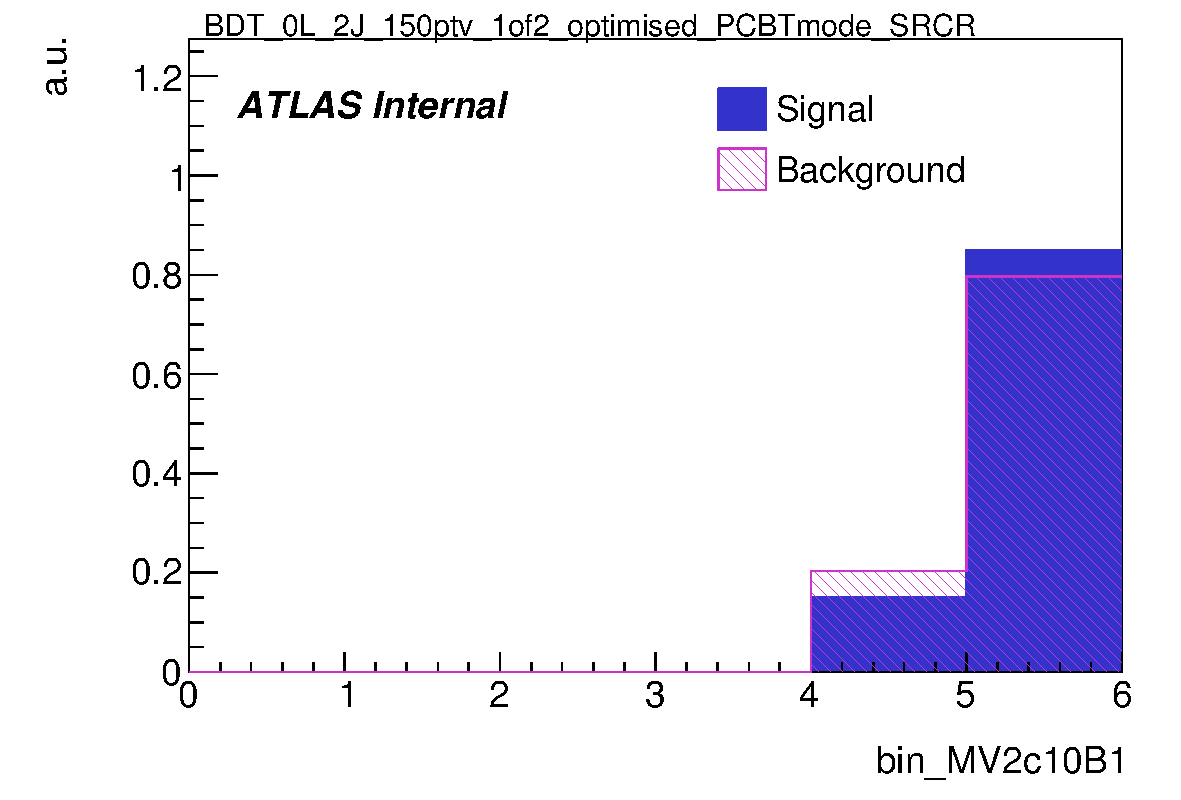
\includegraphics[width=0.33\linewidth]{0-lep-mva/Distr_SignalBackground_bin_MV2c10B1_BDT_0L_2J_150ptv_1of2_optimised_PCBTmode_SRCR-eps-converted-to}}
    \subfloat[]{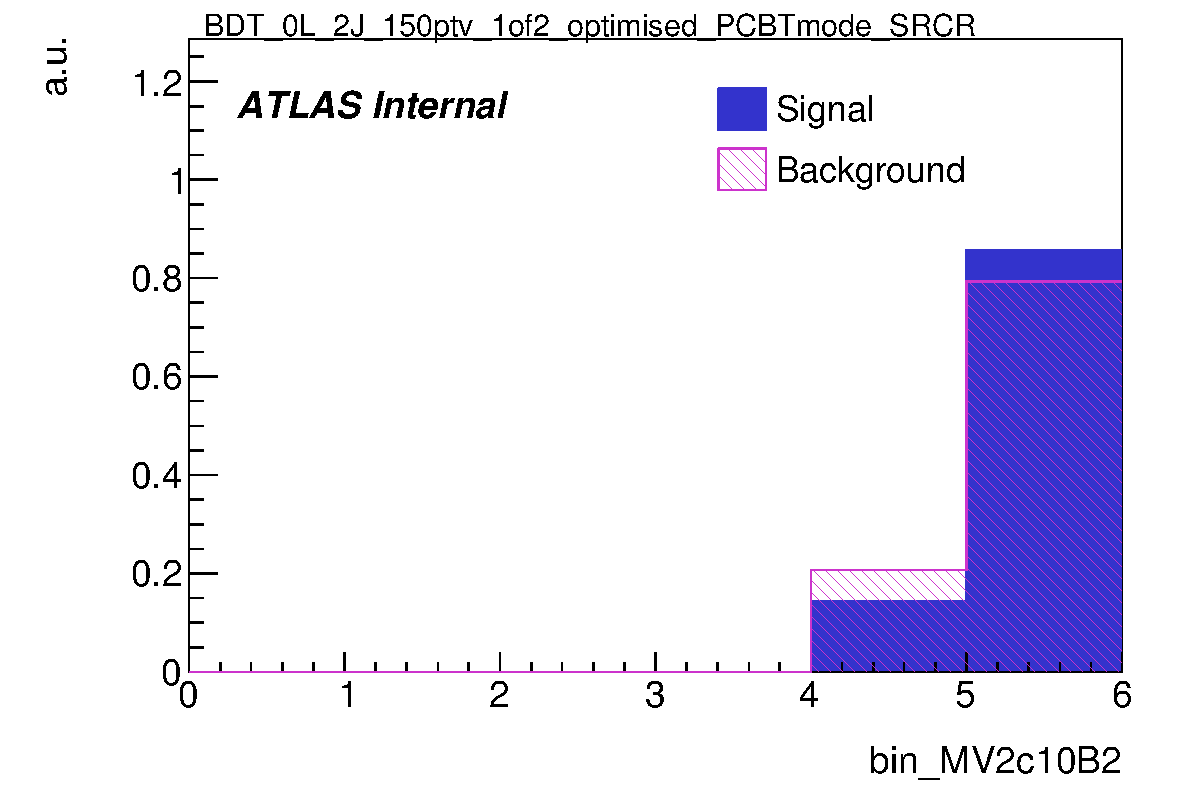
\includegraphics[width=0.33\linewidth]{0-lep-mva/Distr_SignalBackground_bin_MV2c10B2_BDT_0L_2J_150ptv_1of2_optimised_PCBTmode_SRCR-eps-converted-to}}
     \subfloat[]{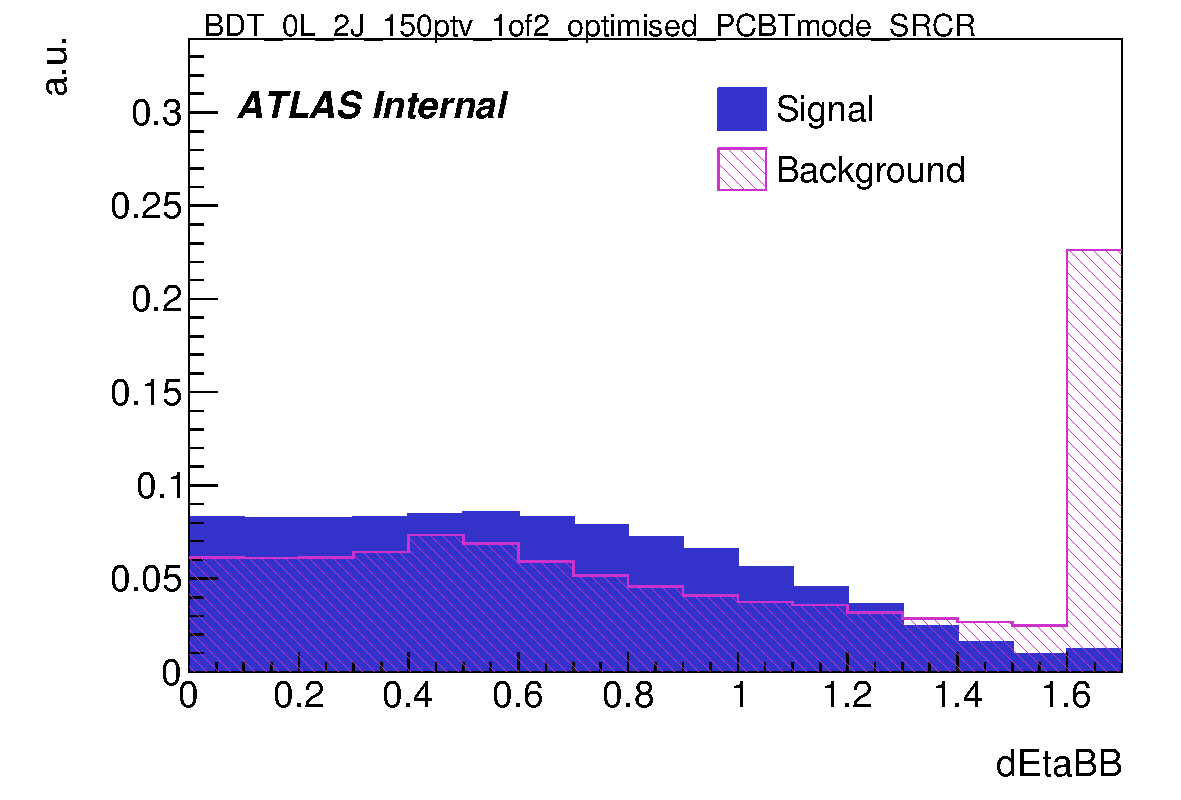
\includegraphics[width=0.33\linewidth]{0-lep-mva/Distr_SignalBackground_dEtaBB_BDT_0L_2J_150ptv_1of2_optimised_PCBTmode_SRCR-eps-converted-to}}\\
    \subfloat[]{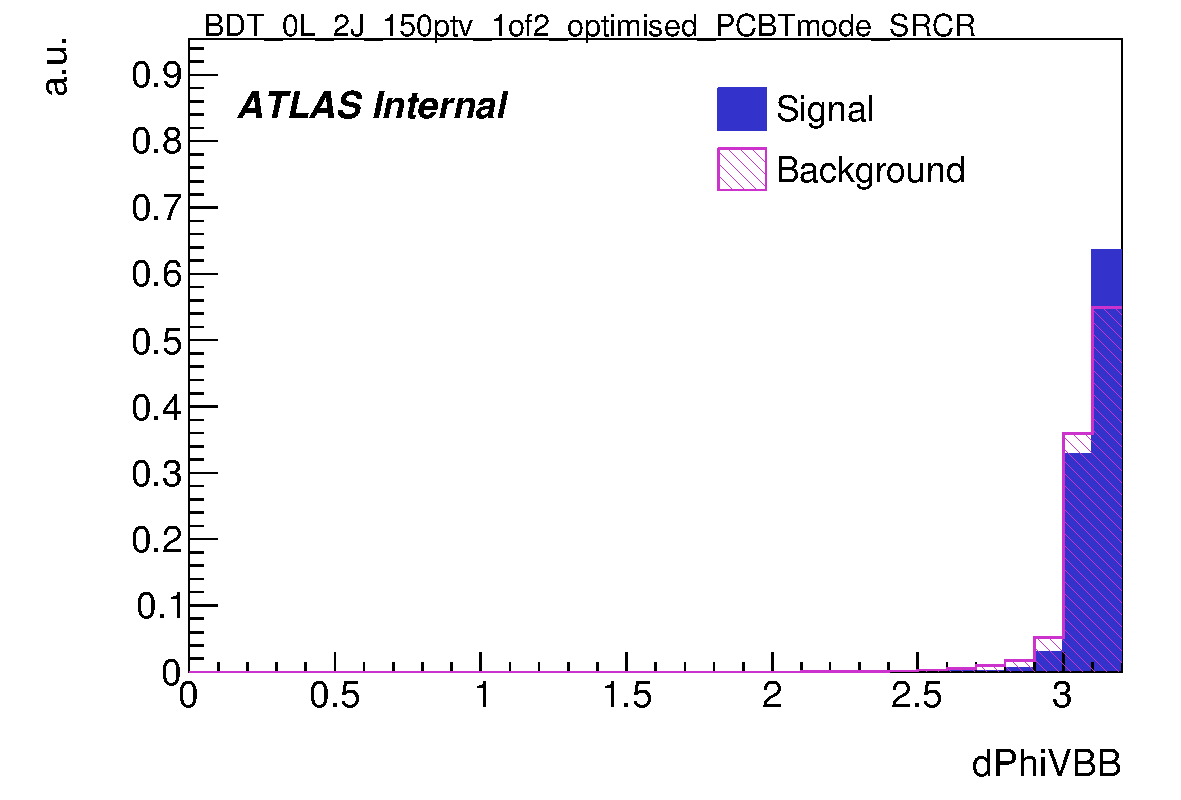
\includegraphics[width=0.33\linewidth]{0-lep-mva/Distr_SignalBackground_dPhiVBB_BDT_0L_2J_150ptv_1of2_optimised_PCBTmode_SRCR-eps-converted-to}}
    \subfloat[]{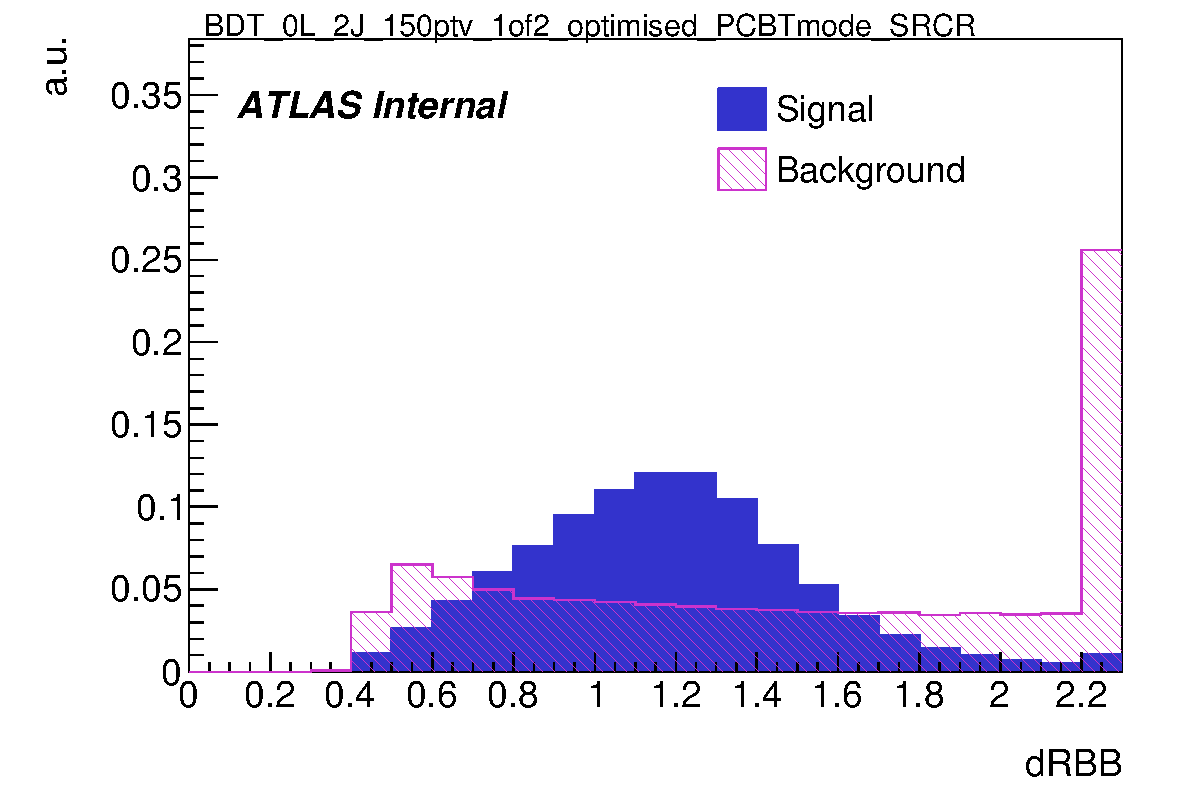
\includegraphics[width=0.33\linewidth]{0-lep-mva/Distr_SignalBackground_dRBB_BDT_0L_2J_150ptv_1of2_optimised_PCBTmode_SRCR-eps-converted-to}}
     \subfloat[]{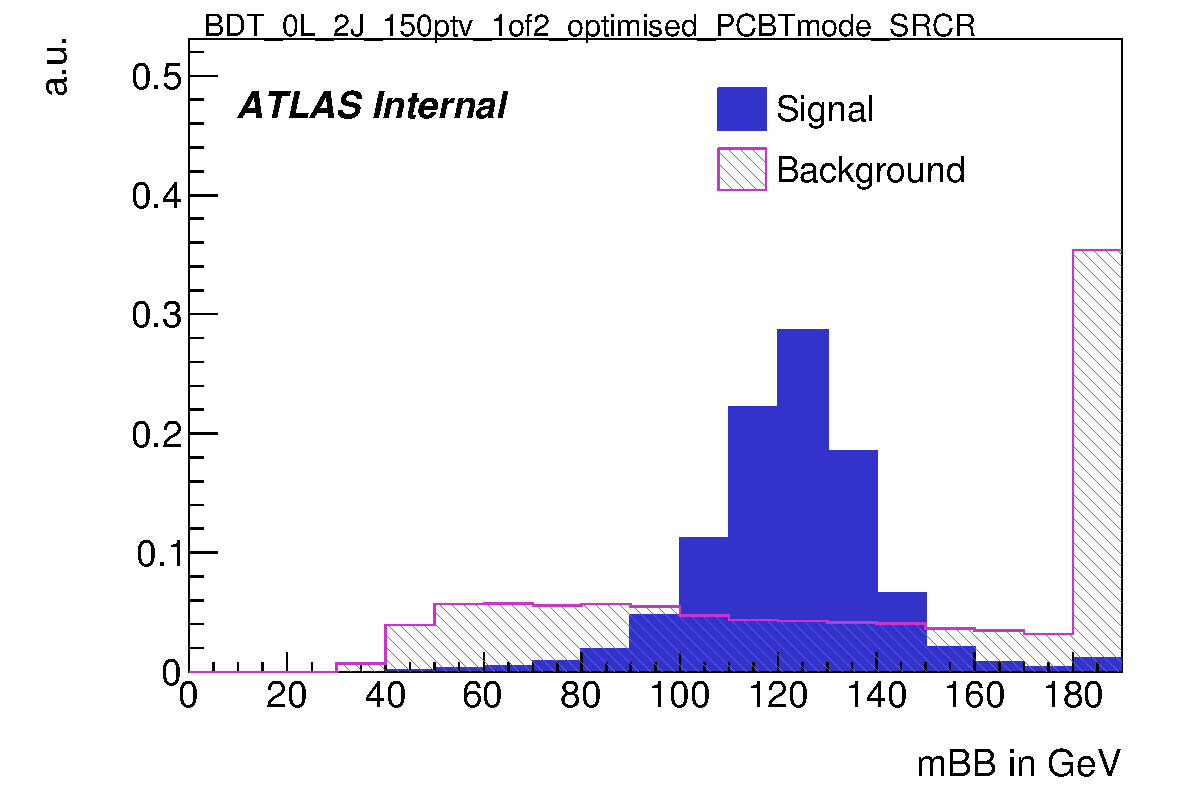
\includegraphics[width=0.33\linewidth]{0-lep-mva/Distr_SignalBackground_mBB_BDT_0L_2J_150ptv_1of2_optimised_PCBTmode_SRCR-eps-converted-to}}\\
    \subfloat[]{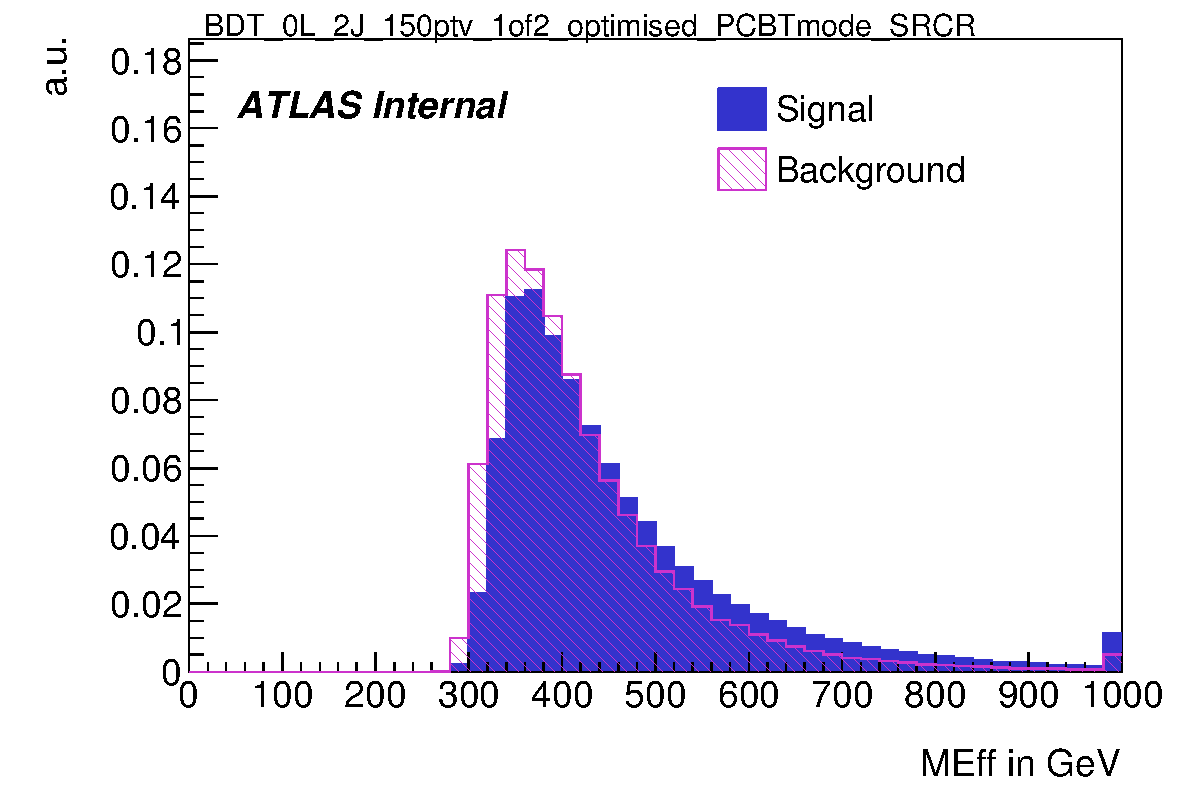
\includegraphics[width=0.33\linewidth]{0-lep-mva/Distr_SignalBackground_MEff_BDT_0L_2J_150ptv_1of2_optimised_PCBTmode_SRCR-eps-converted-to}}
     \subfloat[]{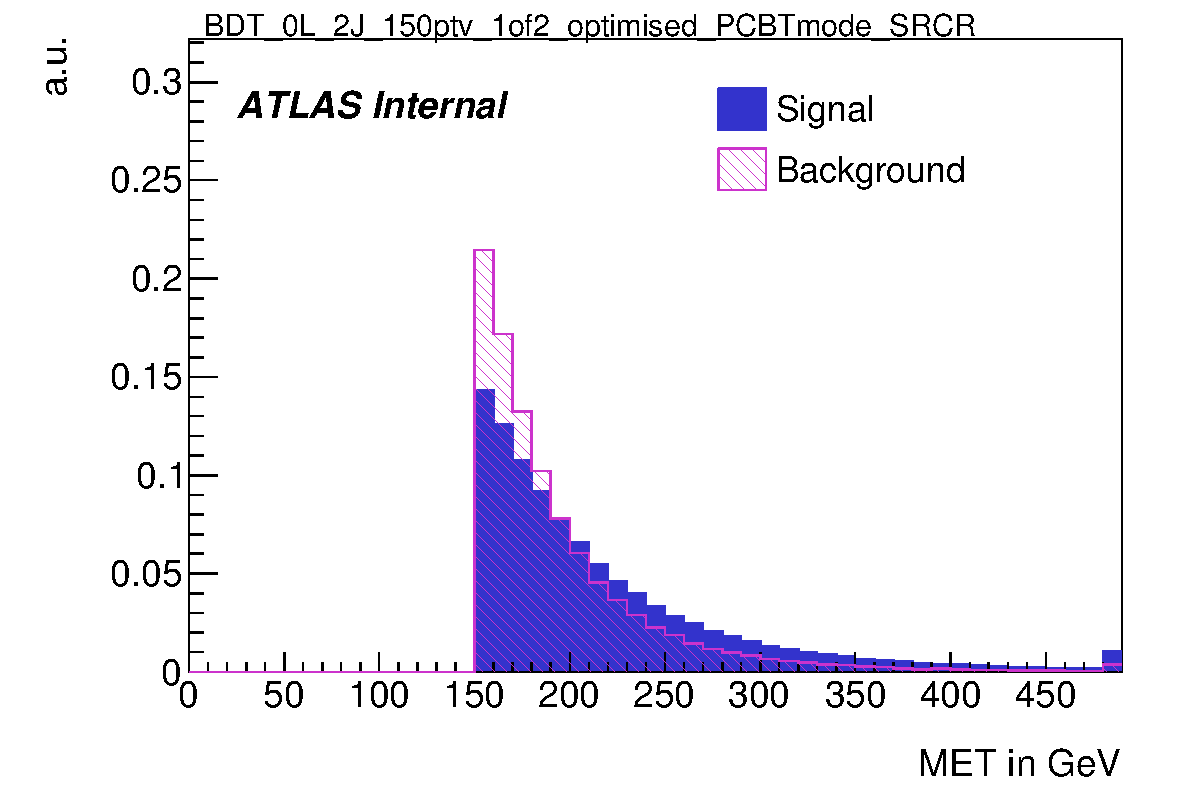
\includegraphics[width=0.33\linewidth]{0-lep-mva/Distr_SignalBackground_MET_BDT_0L_2J_150ptv_1of2_optimised_PCBTmode_SRCR-eps-converted-to}}          
    \subfloat[]{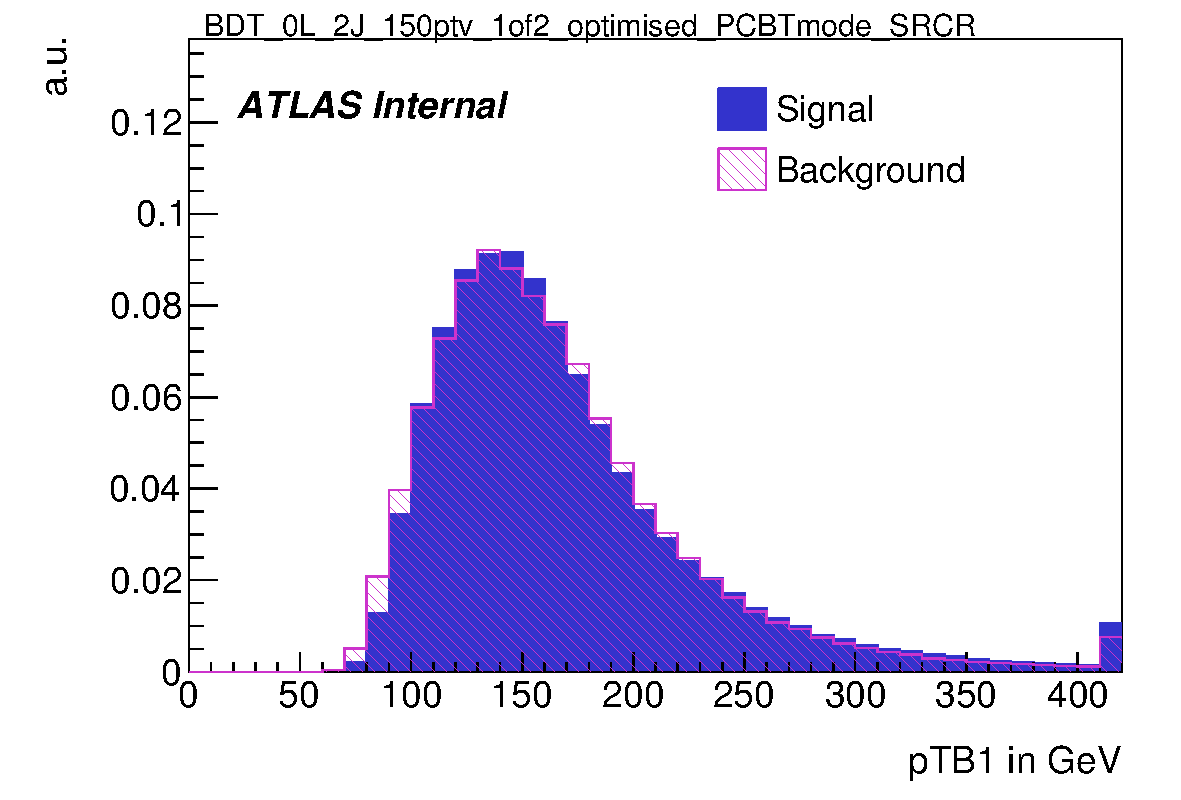
\includegraphics[width=0.33\linewidth]{0-lep-mva/Distr_SignalBackground_pTB1_BDT_0L_2J_150ptv_1of2_optimised_PCBTmode_SRCR-eps-converted-to}} \\
    \subfloat[]{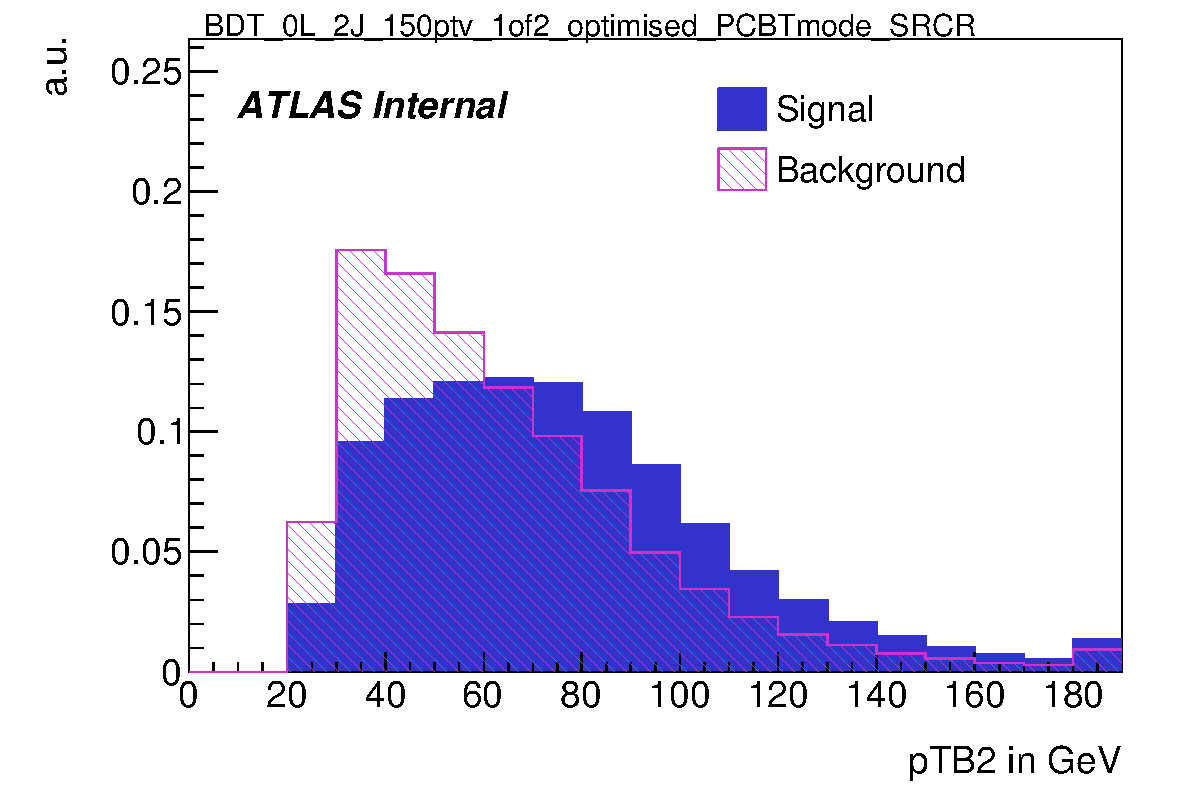
\includegraphics[width=0.33\linewidth]{0-lep-mva/Distr_SignalBackground_pTB2_BDT_0L_2J_150ptv_1of2_optimised_PCBTmode_SRCR-eps-converted-to}}   
    \subfloat[]{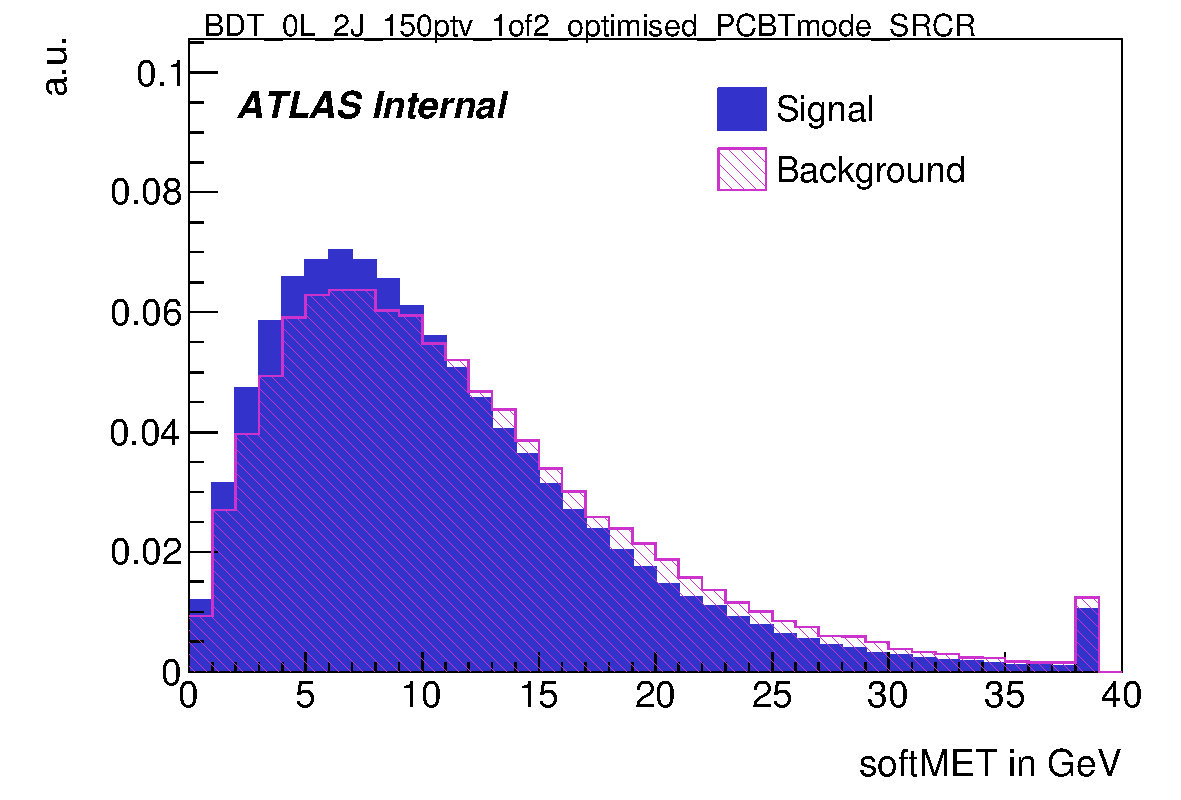
\includegraphics[width=0.33\linewidth]{0-lep-mva/Distr_SignalBackground_softMET_BDT_0L_2J_150ptv_1of2_optimised_PCBTmode_SRCR-eps-converted-to}}\\    
    \end{tabular}
    \caption[Inputs to the multi-variate analysis in the 0--lepton 2--jet
    region.]{Inputs to the multi-variate analysis in the 0--lepton 2--jet
      region. Signal events are shown in blue and background events are shown in
      red. The signal and background histograms have been normalised to the same
      area. The distributions only include events with $E_T^{\text{miss}}$ > 150
      \GeV.}
    \label{fig:bdtinputs-0lep}
\end{figure}

 \begin{figure}[htbp]
  \centering
  \begin{tabular}{cccc}
    \subfloat[]{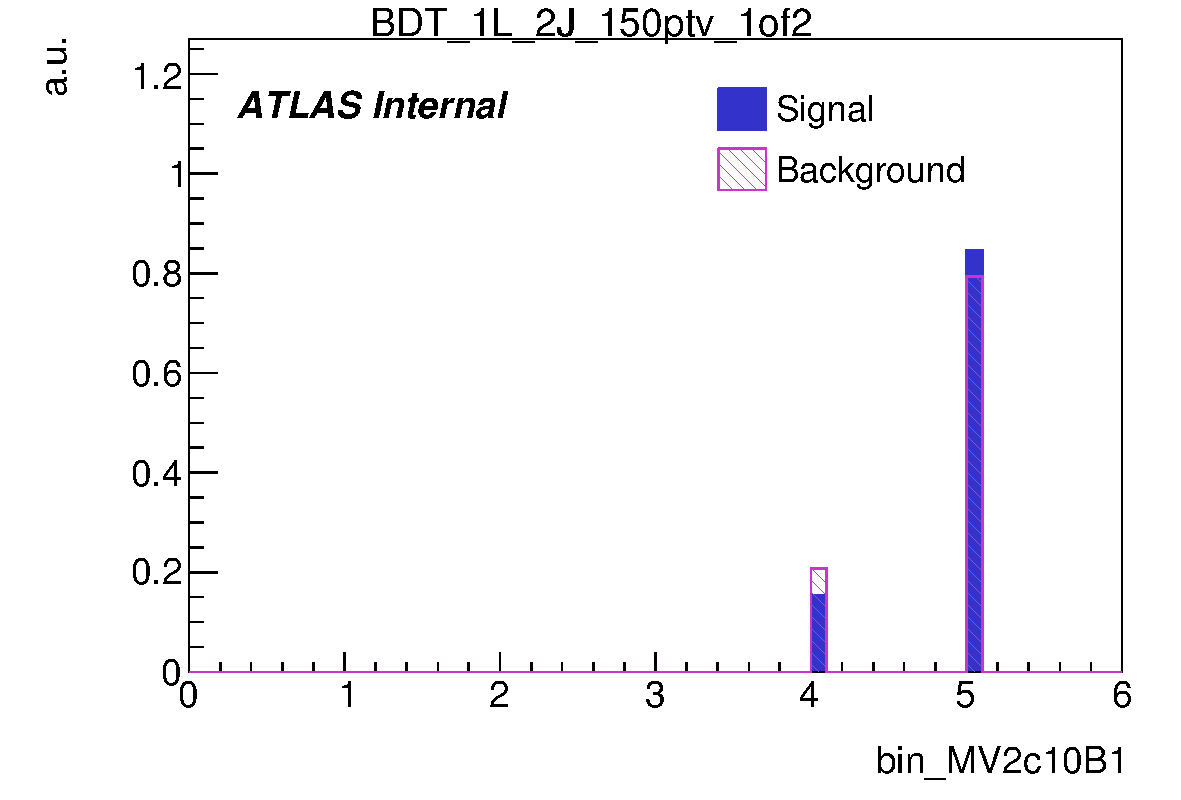
\includegraphics[width=0.3\linewidth]{1-lep-mva/Distr_SignalBackground_bin_MV2c10B1_BDT_1L_2J_150ptv_1of2-eps-converted-to}}
    \subfloat[]{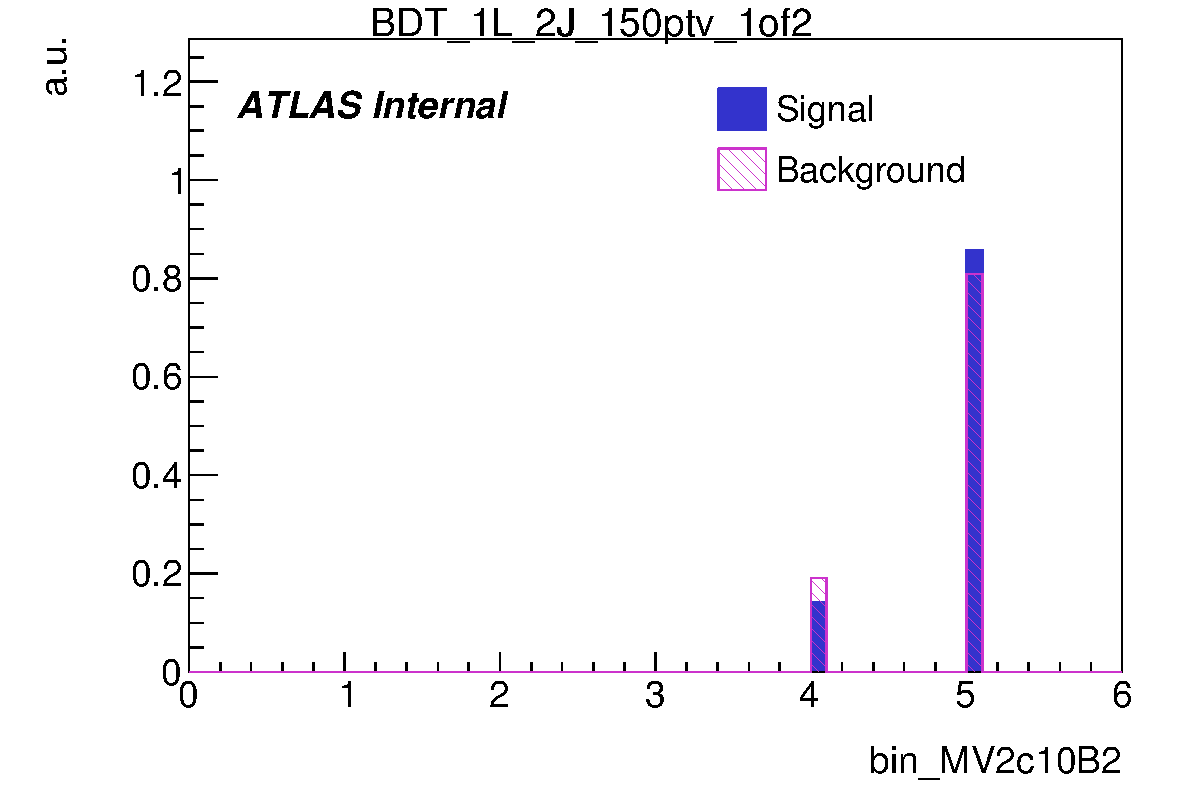
\includegraphics[width=0.3\linewidth]{1-lep-mva/Distr_SignalBackground_bin_MV2c10B2_BDT_1L_2J_150ptv_1of2-eps-converted-to}}
     \subfloat[]{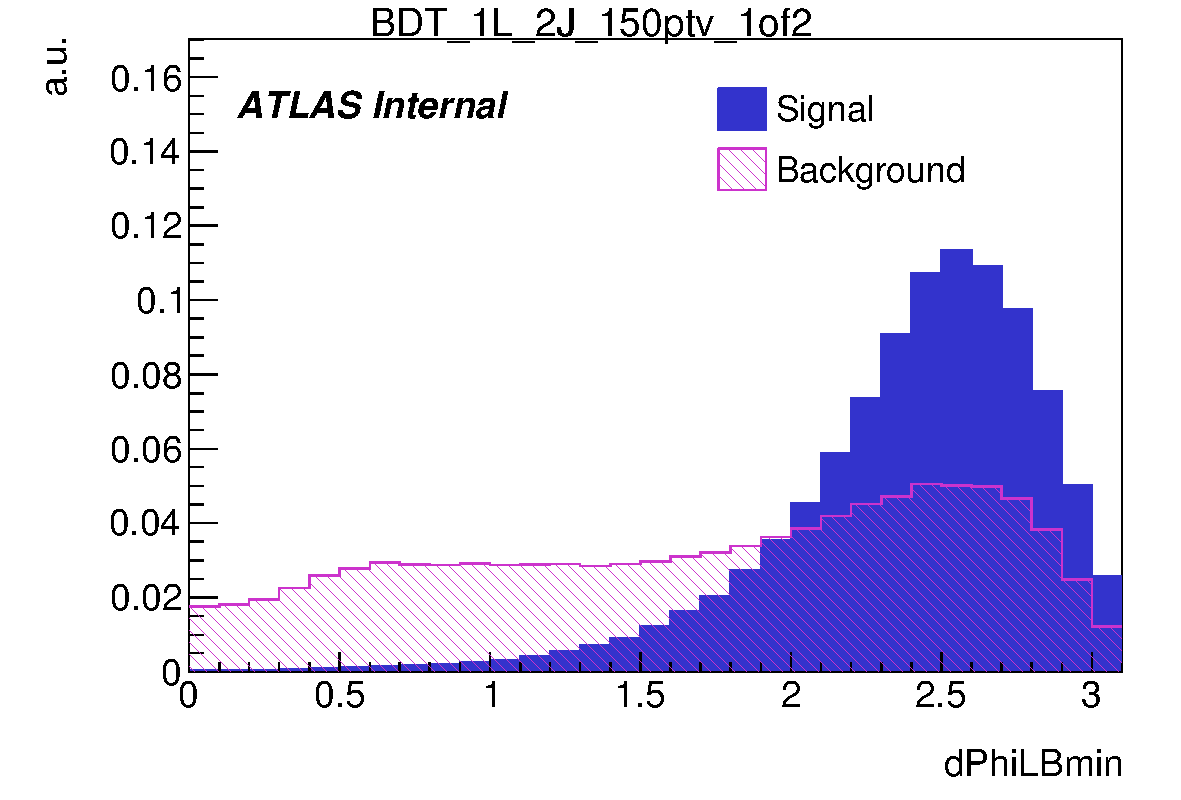
\includegraphics[width=0.3\linewidth]{1-lep-mva/Distr_SignalBackground_dPhiLBmin_BDT_1L_2J_150ptv_1of2-eps-converted-to}}\\
    \subfloat[]{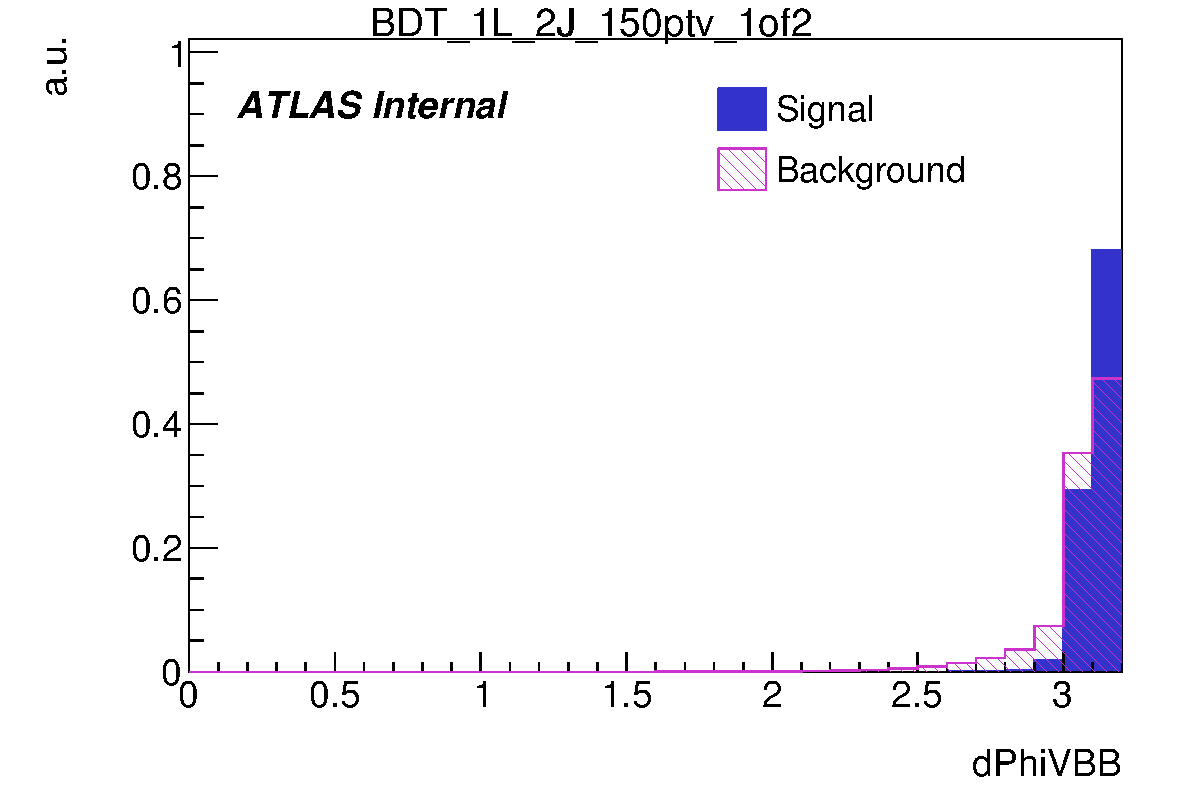
\includegraphics[width=0.3\linewidth]{1-lep-mva/Distr_SignalBackground_dPhiVBB_BDT_1L_2J_150ptv_1of2-eps-converted-to}}
    \subfloat[]{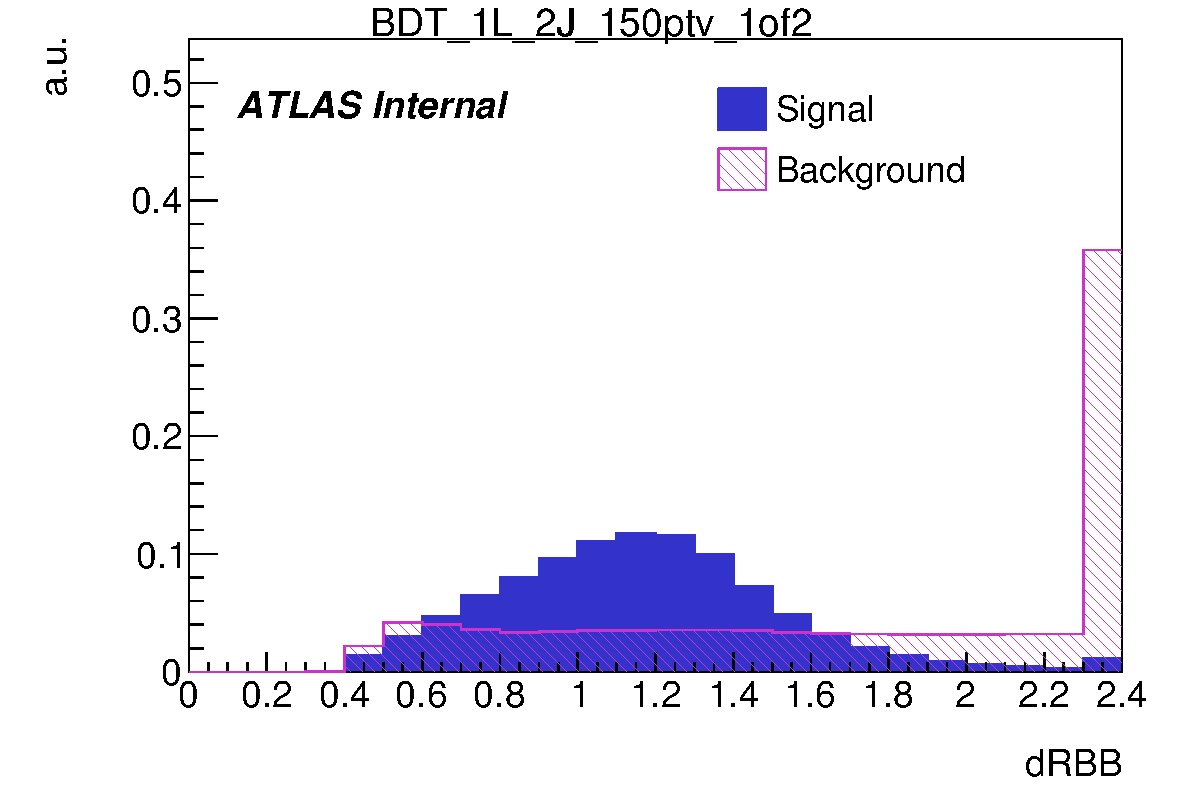
\includegraphics[width=0.3\linewidth]{1-lep-mva/Distr_SignalBackground_dRBB_BDT_1L_2J_150ptv_1of2-eps-converted-to}}
     \subfloat[]{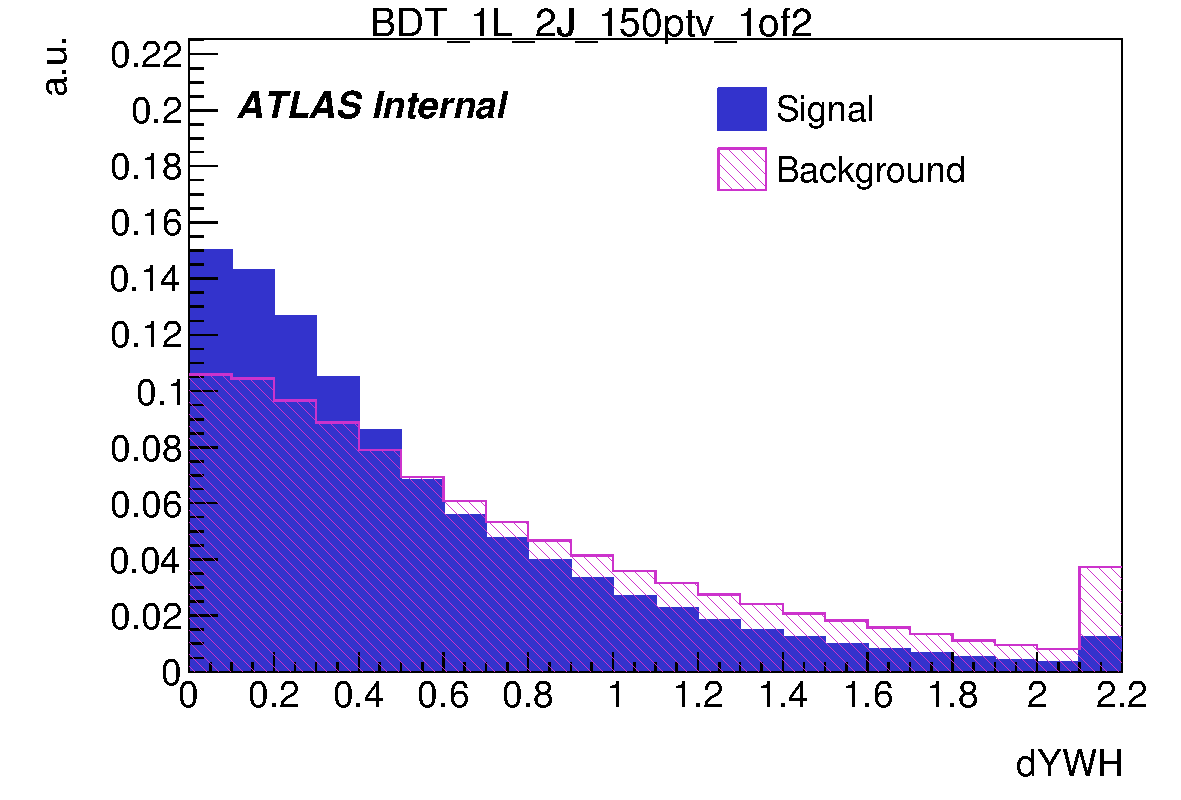
\includegraphics[width=0.3\linewidth]{1-lep-mva/Distr_SignalBackground_dYWH_BDT_1L_2J_150ptv_1of2-eps-converted-to}}\\
    \subfloat[]{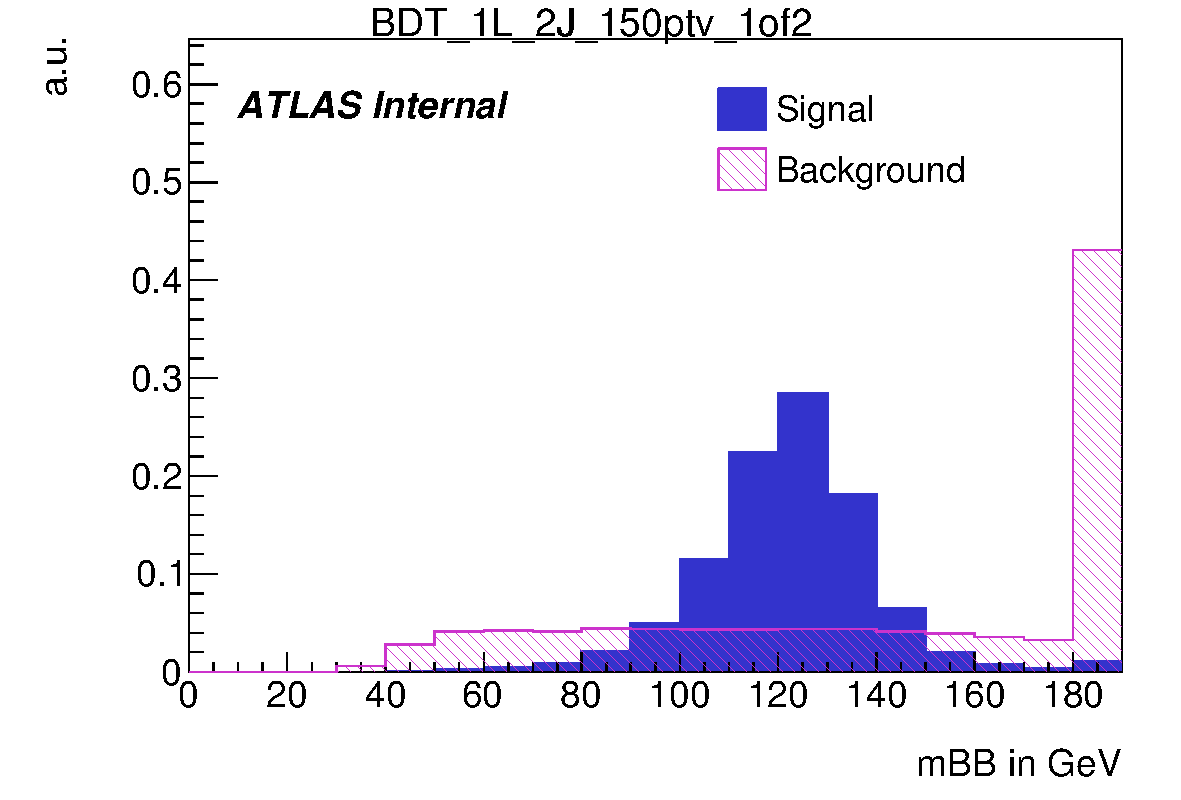
\includegraphics[width=0.3\linewidth]{1-lep-mva/Distr_SignalBackground_mBB_BDT_1L_2J_150ptv_1of2-eps-converted-to}}
     \subfloat[]{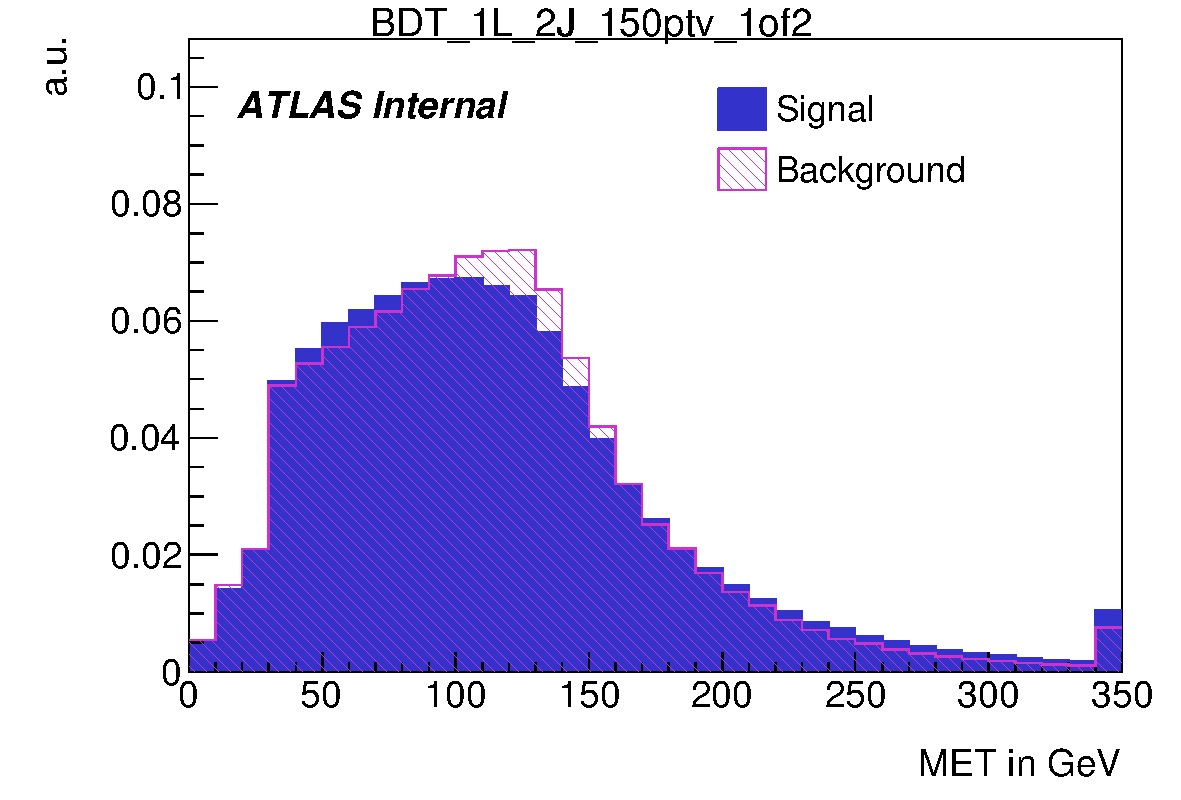
\includegraphics[width=0.3\linewidth]{1-lep-mva/Distr_SignalBackground_MET_BDT_1L_2J_150ptv_1of2-eps-converted-to}}          
    \subfloat[]{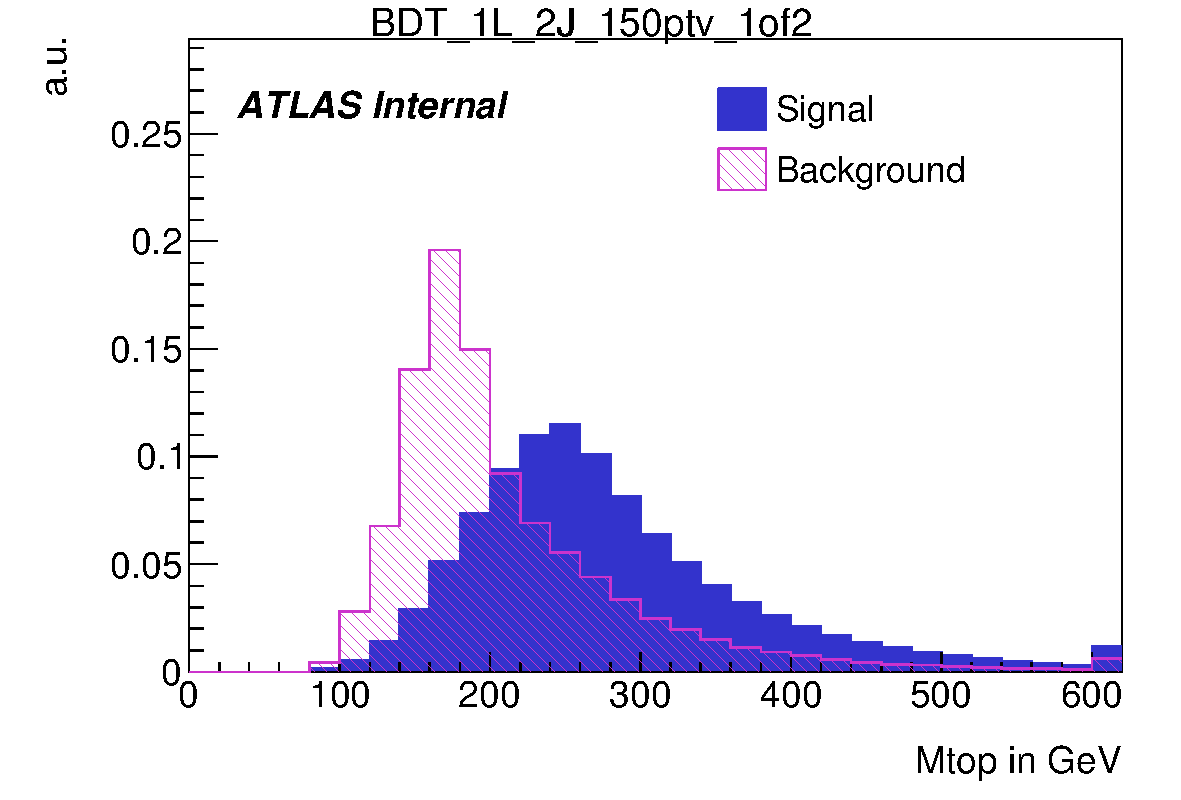
\includegraphics[width=0.3\linewidth]{1-lep-mva/Distr_SignalBackground_Mtop_BDT_1L_2J_150ptv_1of2-eps-converted-to}} \\
    \subfloat[]{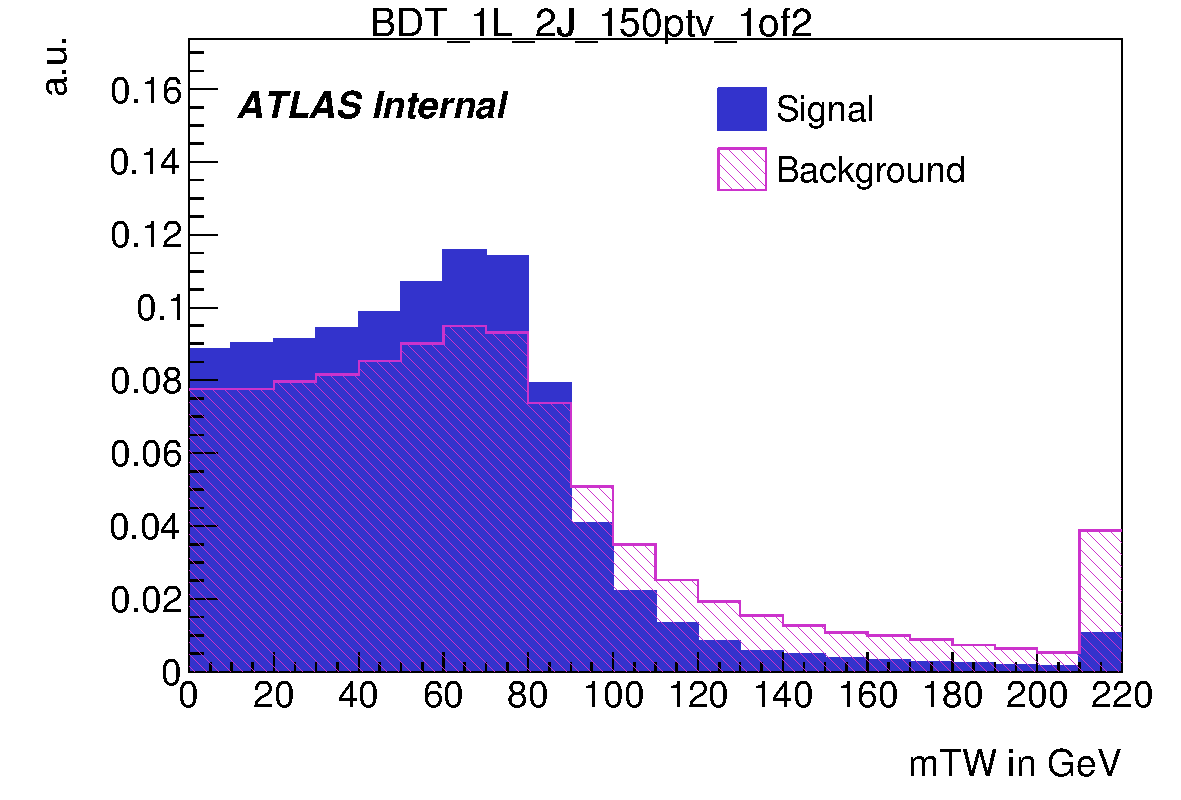
\includegraphics[width=0.3\linewidth]{1-lep-mva/Distr_SignalBackground_mTW_BDT_1L_2J_150ptv_1of2-eps-converted-to}}   
    \subfloat[]{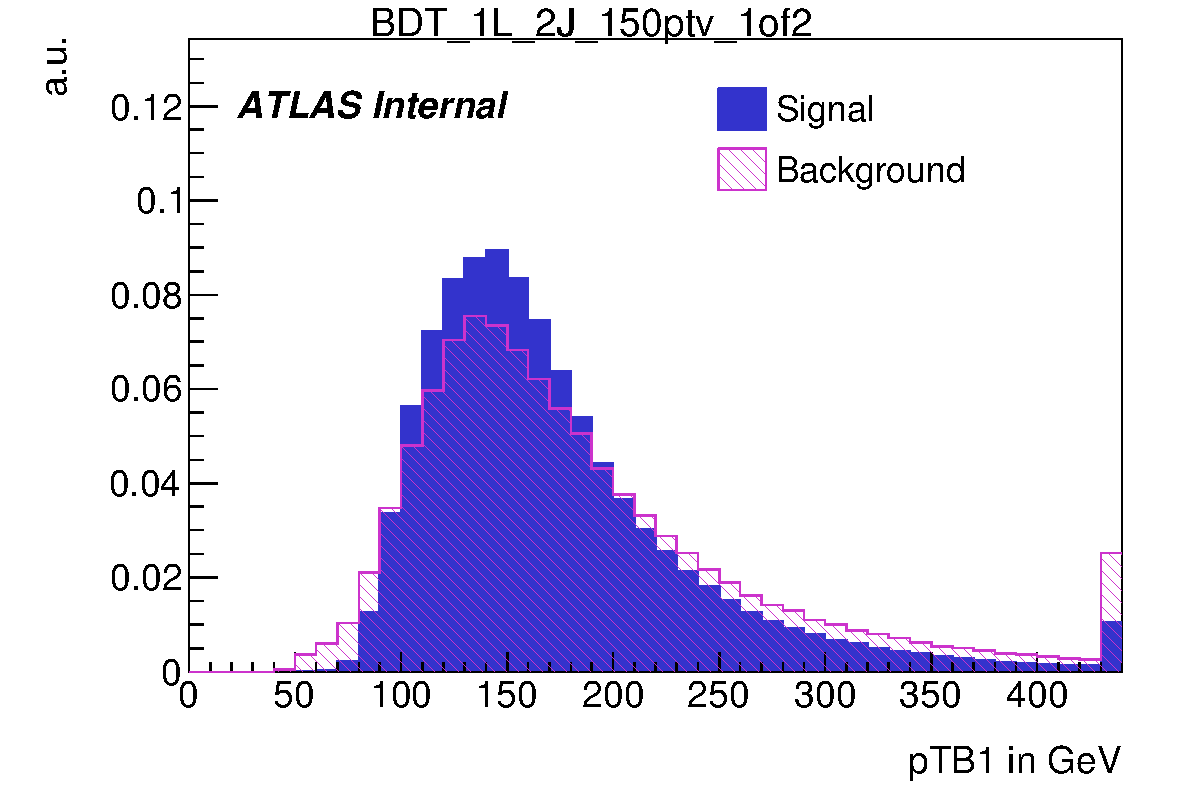
\includegraphics[width=0.3\linewidth]{1-lep-mva/Distr_SignalBackground_pTB1_BDT_1L_2J_150ptv_1of2-eps-converted-to}}
    \subfloat[]{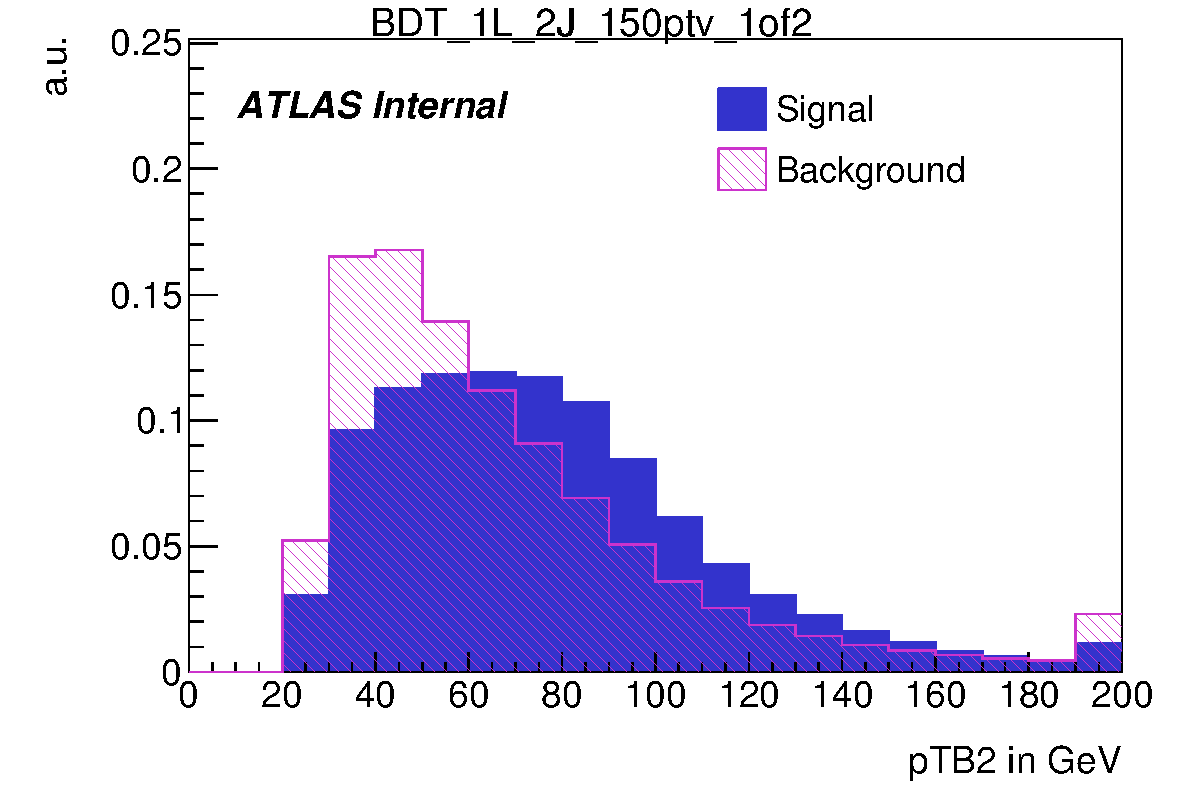
\includegraphics[width=0.3\linewidth]{1-lep-mva/Distr_SignalBackground_pTB2_BDT_1L_2J_150ptv_1of2-eps-converted-to}}\\   
    \subfloat[]{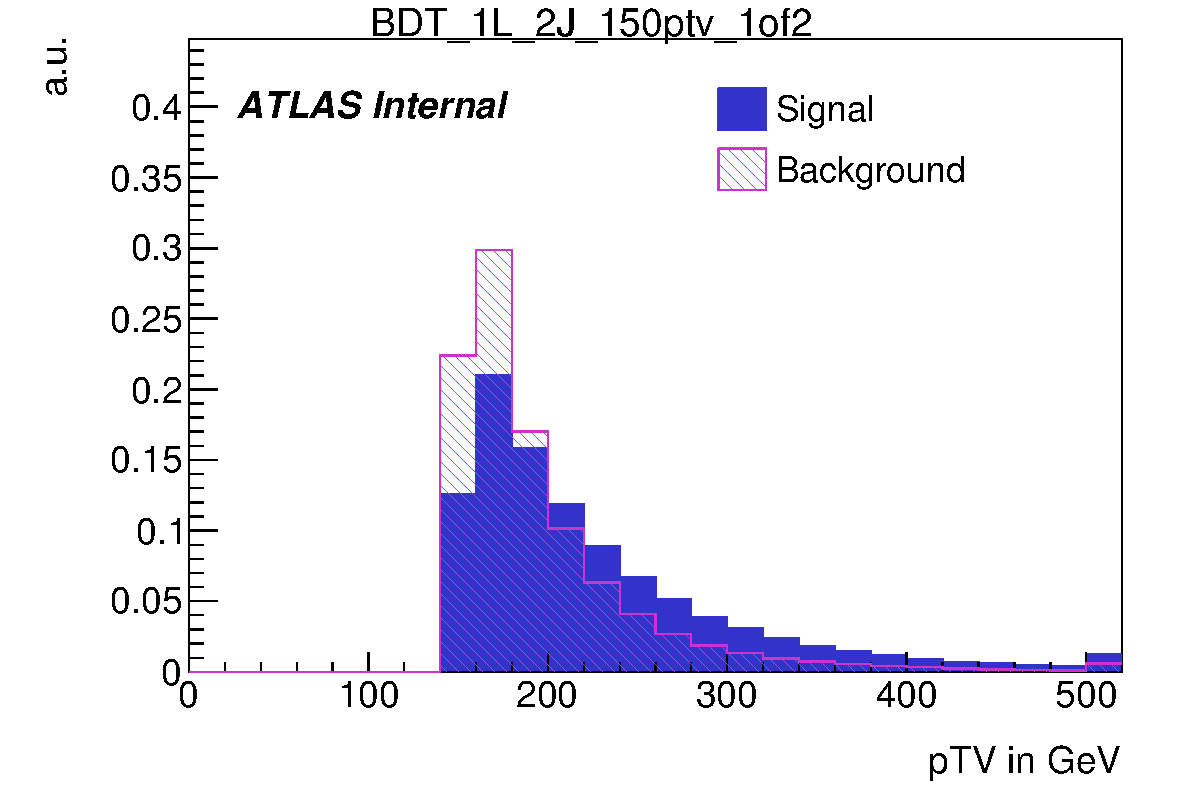
\includegraphics[width=0.3\linewidth]{1-lep-mva/Distr_SignalBackground_pTV_BDT_1L_2J_150ptv_1of2-eps-converted-to}} 
    \end{tabular}
    \caption[Inputs to the multi-variate analysis in the 1--lepton 2--jet
    region.]{Inputs to the multi-variate analysis in the 1--lepton 2--jet
      region. Signal events are shown in blue and background events are shown in
      red. The signal and background histograms have been normalised to the same
      area.The distributions only include events with $p_T^{W}$ > 150
      \GeV.}
    \label{fig:bdtinputs-1lep}
\end{figure}

 \begin{figure}[htbp]
  \centering
  \begin{tabular}{cccc}
    \subfloat[]{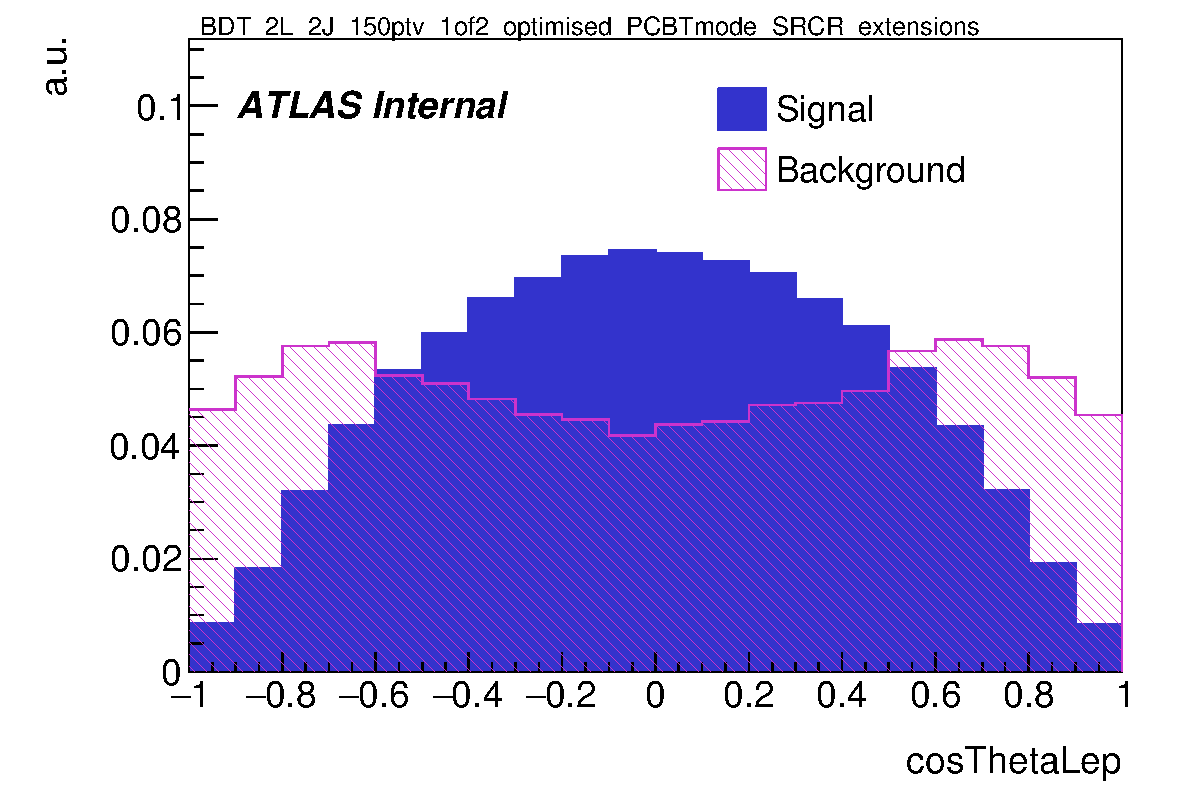
\includegraphics[width=0.33\linewidth]{2-lep-mva/Distr_SignalBackground_cosThetaLep_BDT_2L_2J_150ptv_1of2_optimised_PCBTmode_SRCR_extensions-eps-converted-to}}
    \subfloat[]{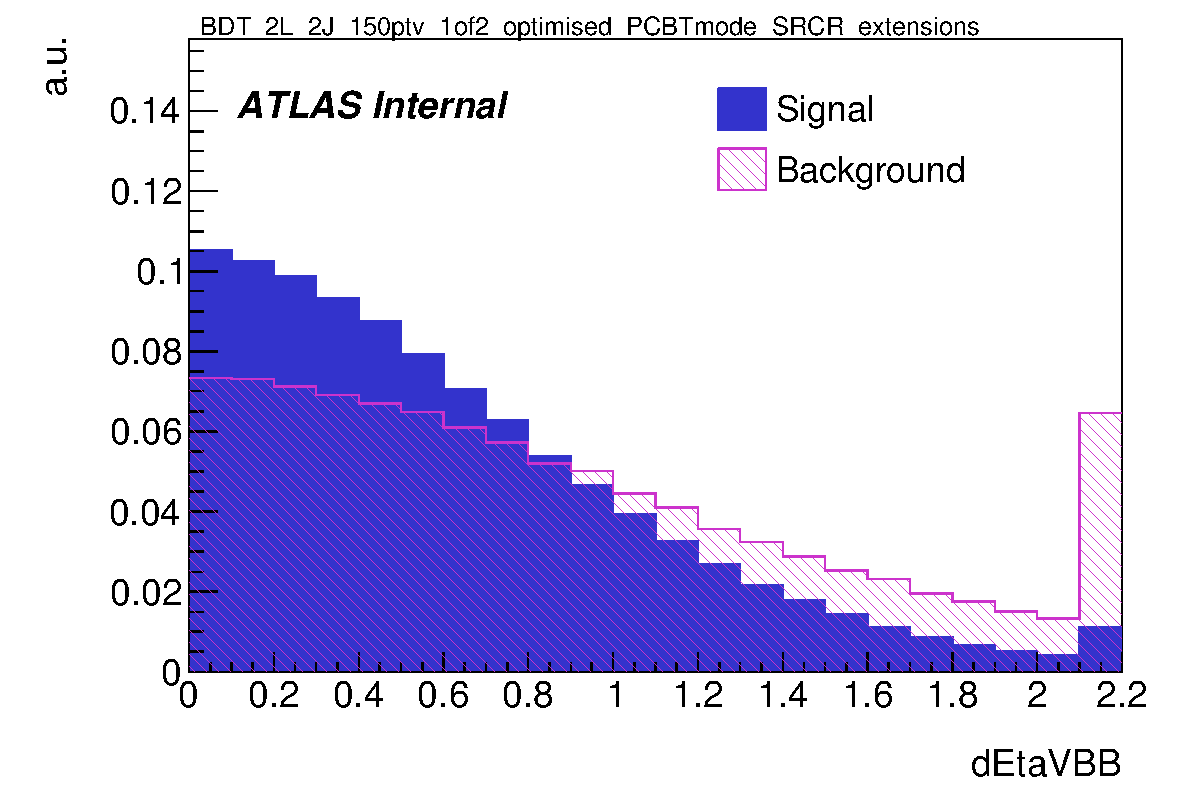
\includegraphics[width=0.33\linewidth]{2-lep-mva/Distr_SignalBackground_dEtaVBB_BDT_2L_2J_150ptv_1of2_optimised_PCBTmode_SRCR_extensions-eps-converted-to}}
     \subfloat[]{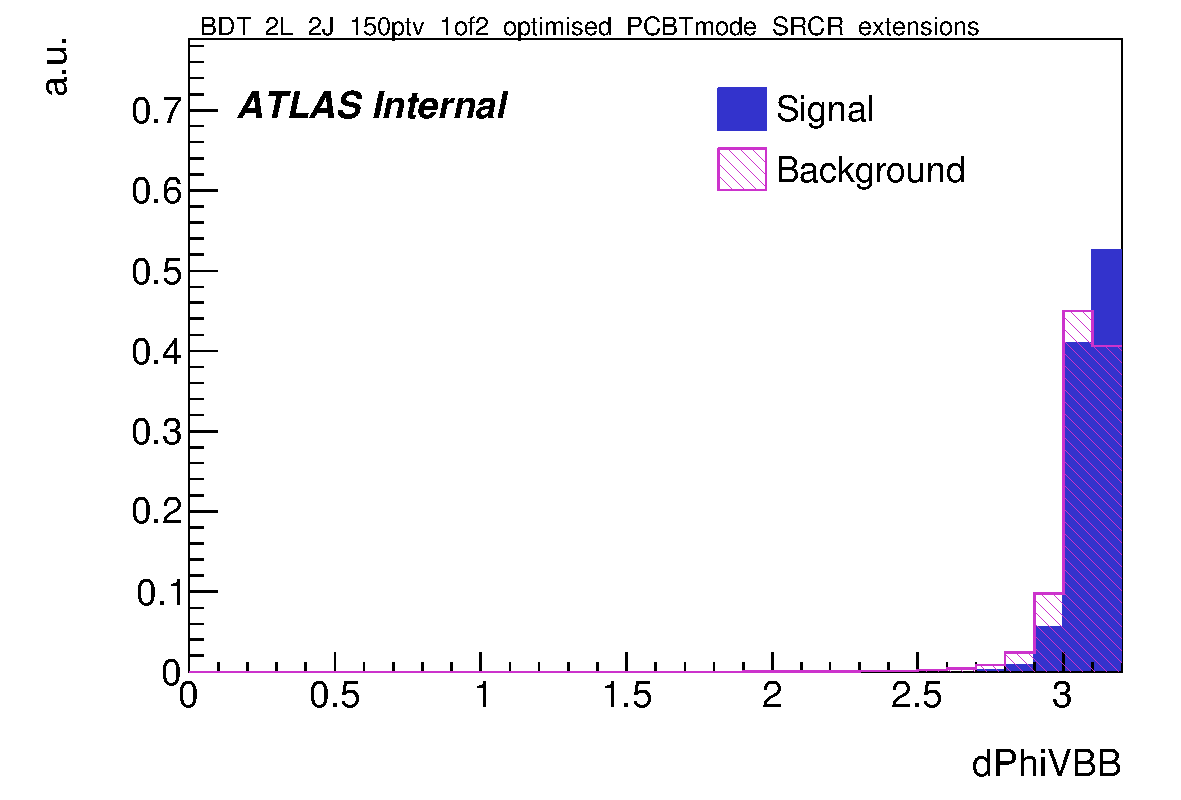
\includegraphics[width=0.33\linewidth]{2-lep-mva/Distr_SignalBackground_dPhiVBB_BDT_2L_2J_150ptv_1of2_optimised_PCBTmode_SRCR_extensions-eps-converted-to}}\\
    \subfloat[]{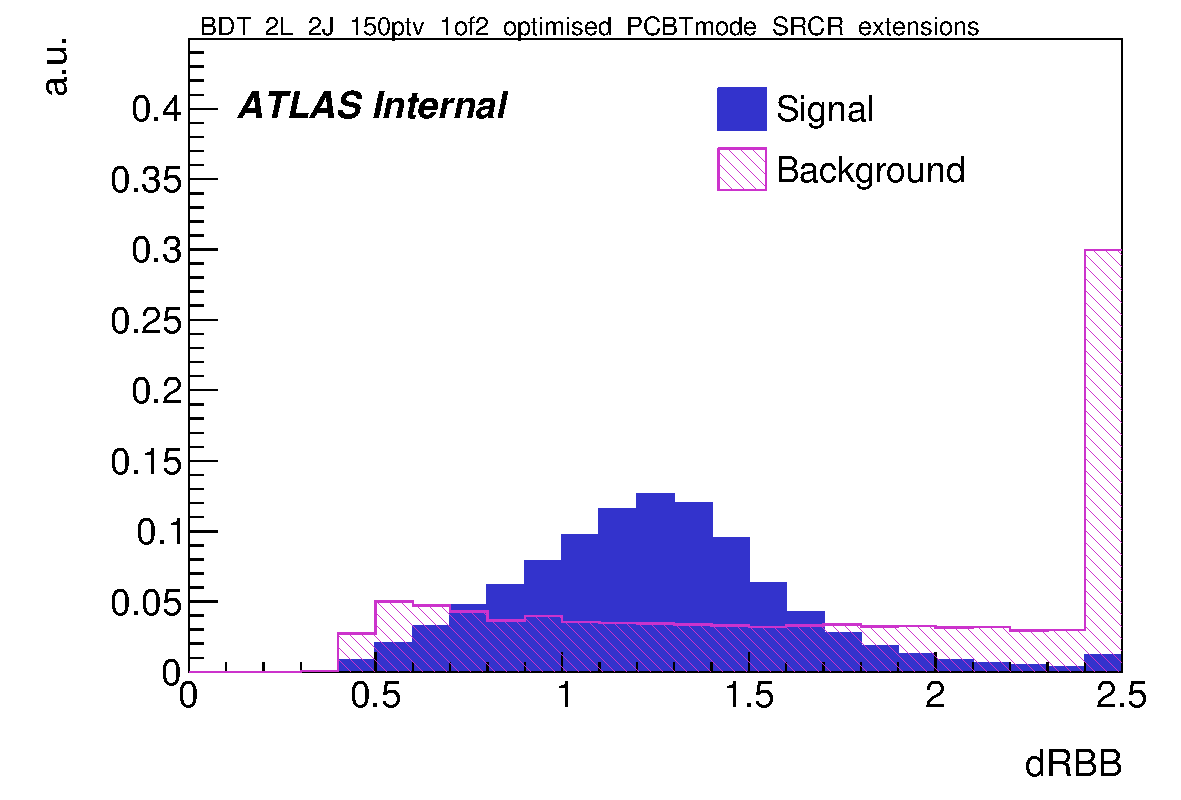
\includegraphics[width=0.33\linewidth]{2-lep-mva/Distr_SignalBackground_dRBB_BDT_2L_2J_150ptv_1of2_optimised_PCBTmode_SRCR_extensions-eps-converted-to}}
    \subfloat[]{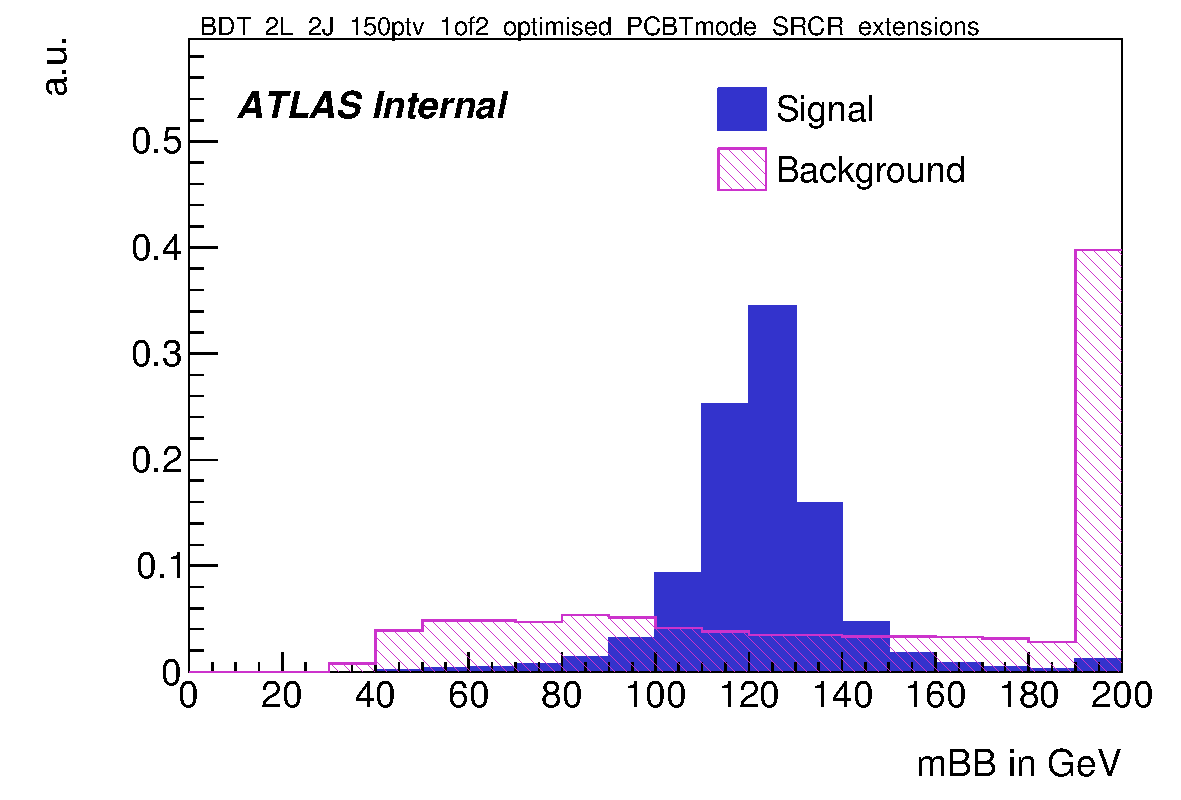
\includegraphics[width=0.33\linewidth]{2-lep-mva/Distr_SignalBackground_mBB_BDT_2L_2J_150ptv_1of2_optimised_PCBTmode_SRCR_extensions-eps-converted-to}}
     \subfloat[]{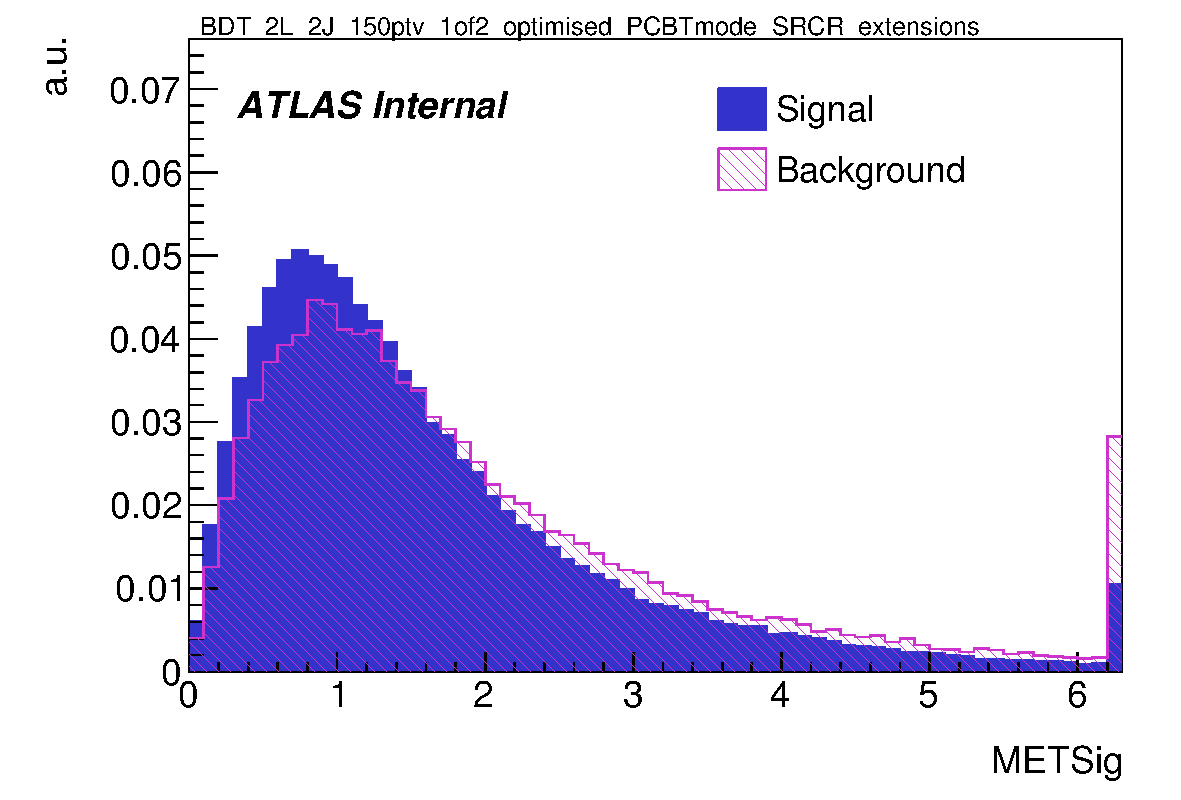
\includegraphics[width=0.33\linewidth]{2-lep-mva/Distr_SignalBackground_METSig_BDT_2L_2J_150ptv_1of2_optimised_PCBTmode_SRCR_extensions-eps-converted-to}}\\
    \subfloat[]{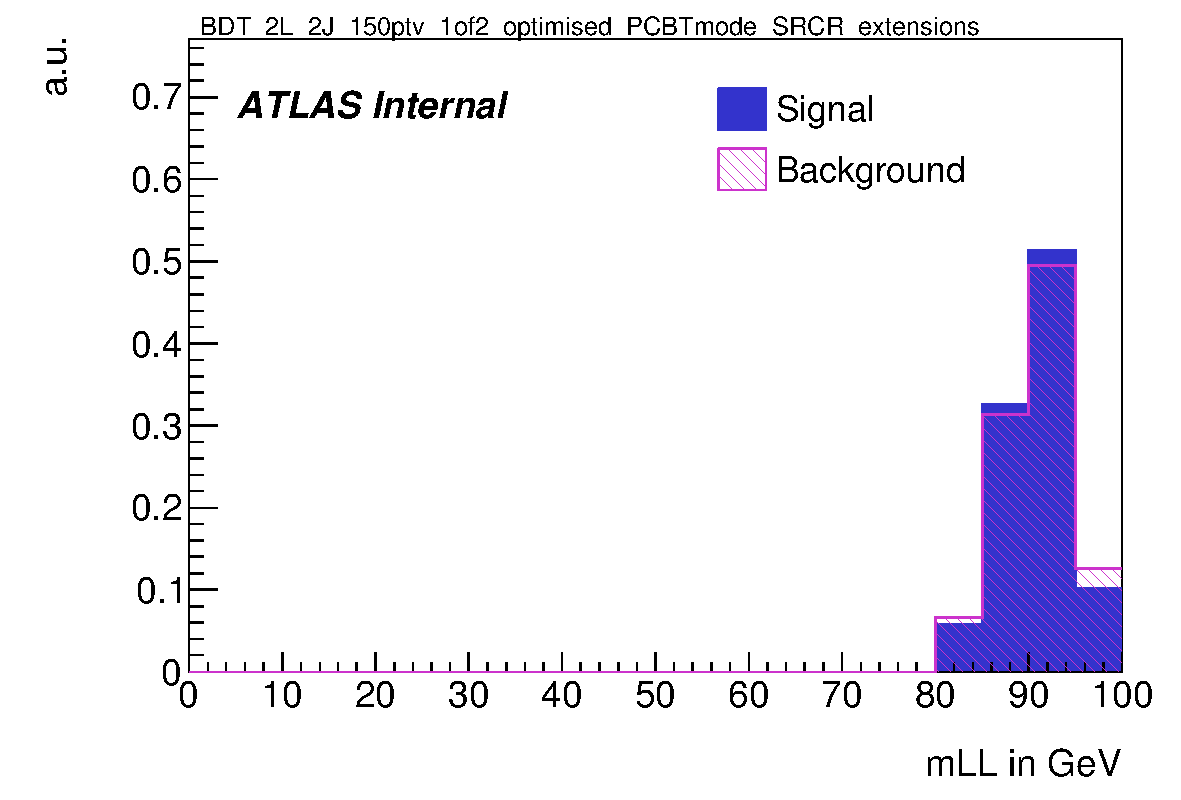
\includegraphics[width=0.33\linewidth]{2-lep-mva/Distr_SignalBackground_mLL_BDT_2L_2J_150ptv_1of2_optimised_PCBTmode_SRCR_extensions-eps-converted-to}}
     \subfloat[]{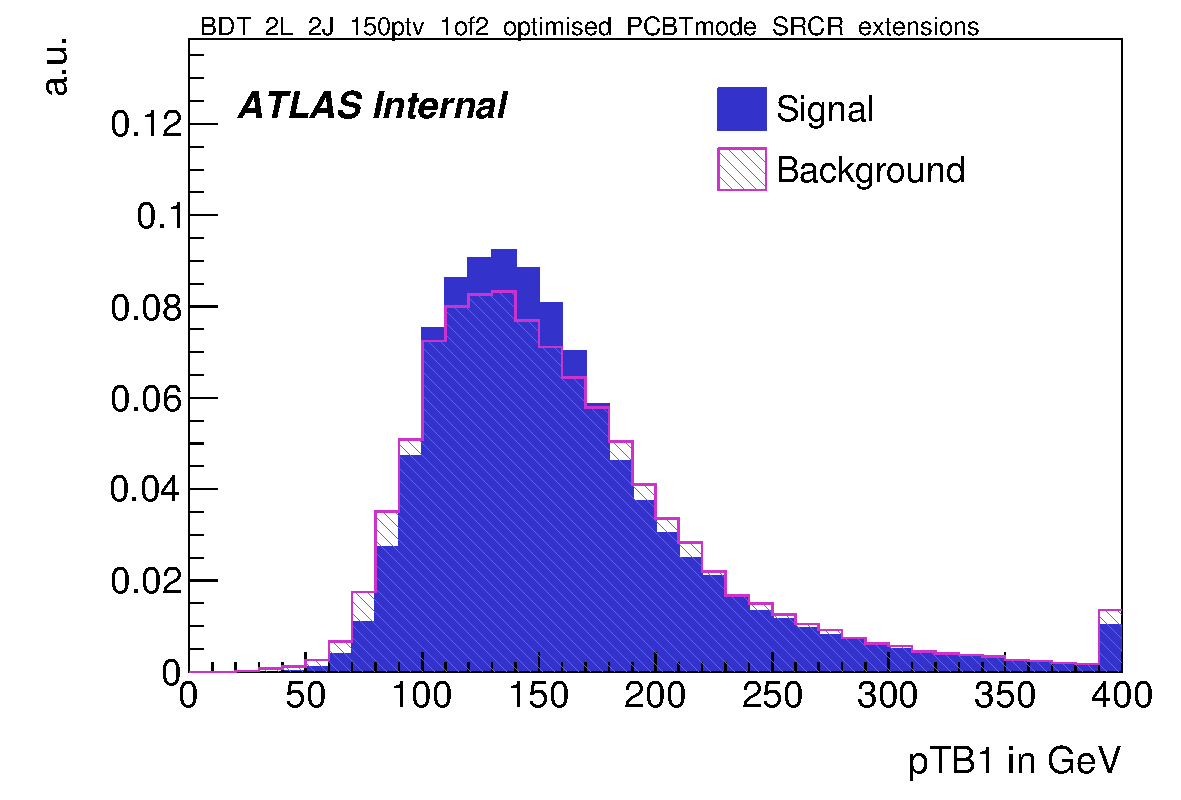
\includegraphics[width=0.33\linewidth]{2-lep-mva/Distr_SignalBackground_pTB1_BDT_2L_2J_150ptv_1of2_optimised_PCBTmode_SRCR_extensions-eps-converted-to}}          
    \subfloat[]{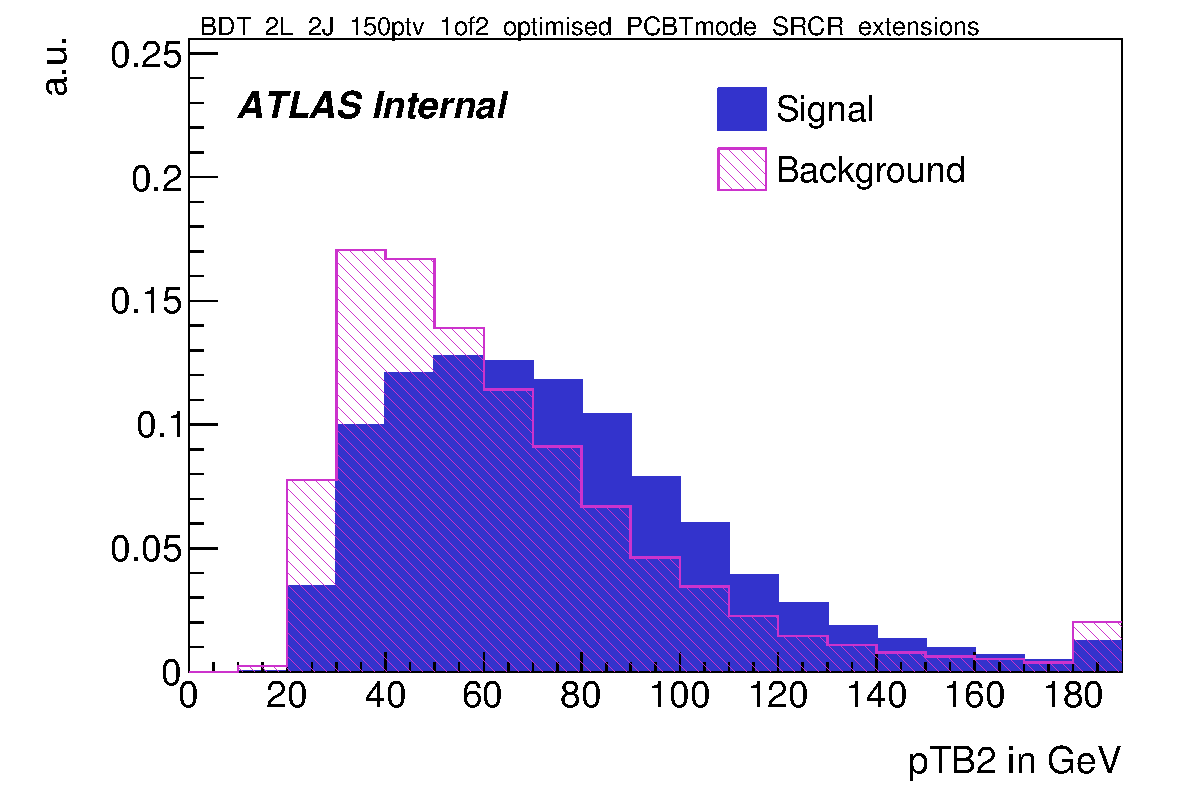
\includegraphics[width=0.33\linewidth]{2-lep-mva/Distr_SignalBackground_pTB2_BDT_2L_2J_150ptv_1of2_optimised_PCBTmode_SRCR_extensions-eps-converted-to}} \\
    \subfloat[]{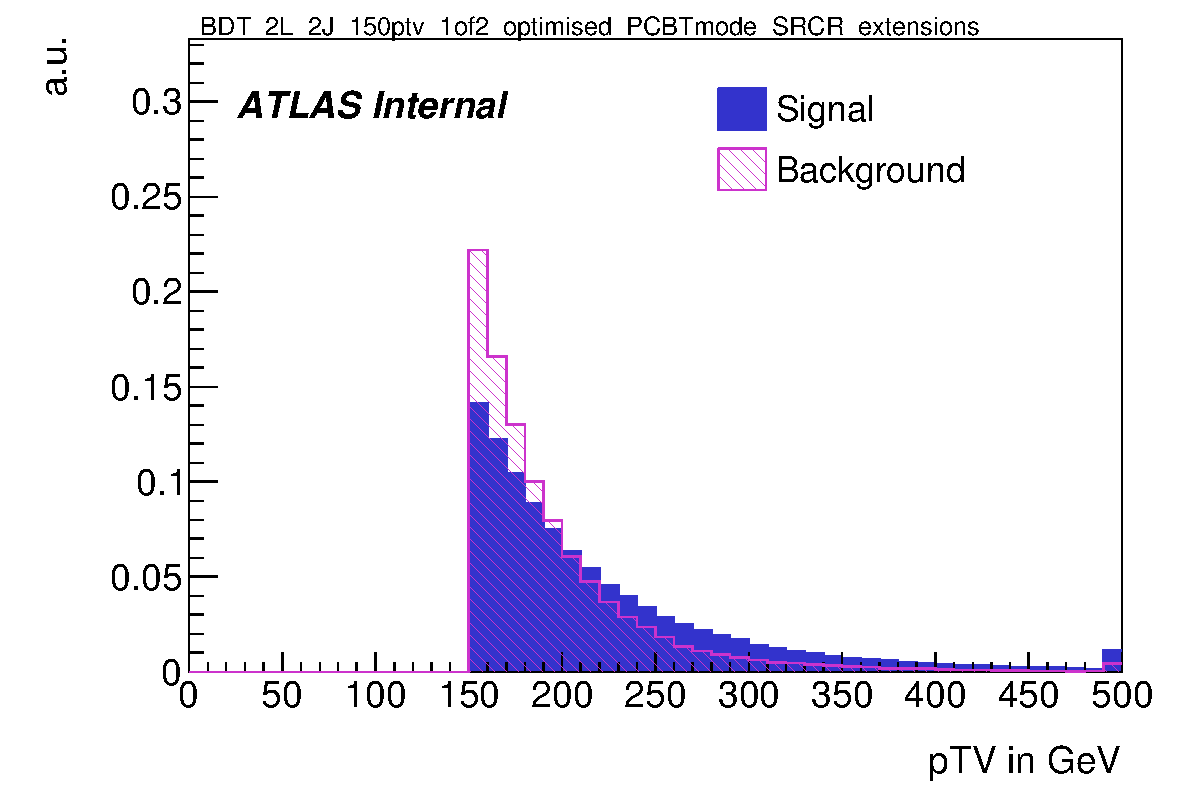
\includegraphics[width=0.33\linewidth]{2-lep-mva/Distr_SignalBackground_pTV_BDT_2L_2J_150ptv_1of2_optimised_PCBTmode_SRCR_extensions-eps-converted-to}}   
    \end{tabular}
    \caption[Inputs to the multi-variate analysis in the 2--lepton 2--jet
    region.]{Inputs to the multi-variate analysis in the 2--lepton 2--jet
      region. Signal events are shown in blue and background events are shown in
      red. The signal and background histograms have been normalised to the same
      area.The distributions only include events with $p_T^{Z}$ > 150
      \GeV.}
    \label{fig:bdtinputs-2lep}
\end{figure}

\subsection{\texorpdfstring{$\Delta R(b,b)$}{DRbb} Control Regions}%
\label{sec:control-region-defintions}
\begin{figure}[h]
  \centering
  \begin{tabular}{cc}
    \subfloat[]{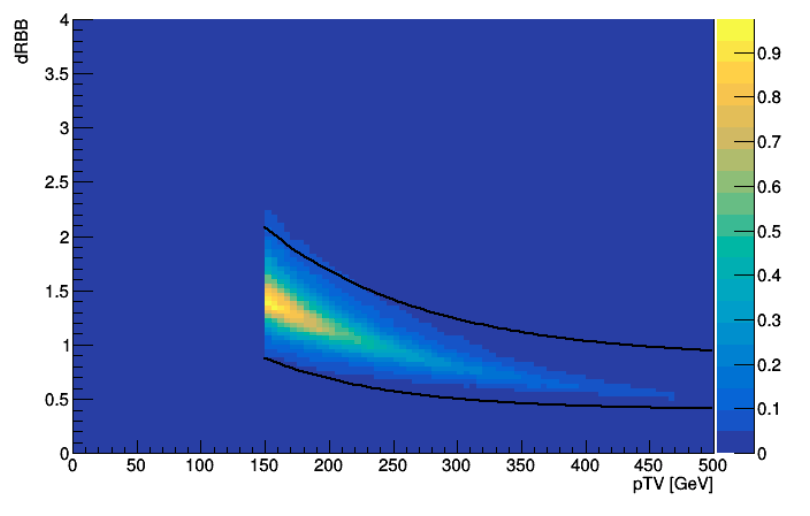
\includegraphics[width=0.505\linewidth]{1lep_qqWH_2tag_2jet.png}}
    \subfloat[]{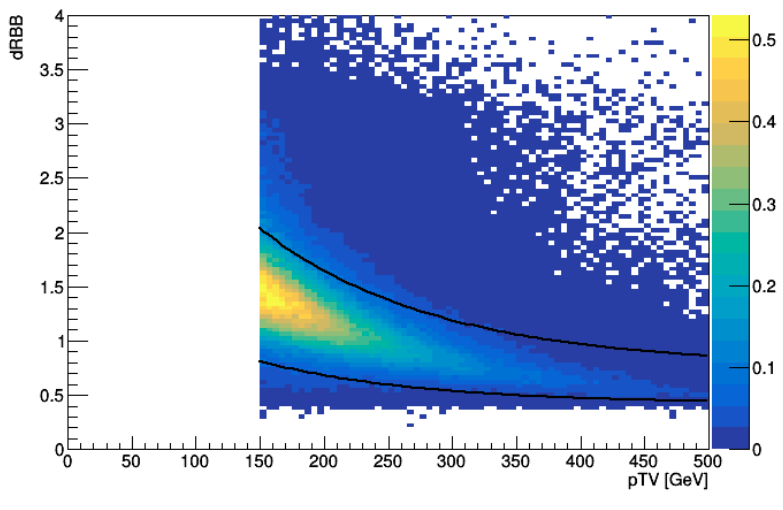
\includegraphics[width=0.49\linewidth]{1lep_qqWH_2tag_3jet.png}}\\
  \end{tabular}
  \caption{Signal distribution of $\Delta R$ between the two selected jets as
    function of $p_{T}^{V}$ in the 1-lepton channel are shown in the 2-tag 2-jet
    (a) and 2-tag 3-jet (b) categories. The black lines demonstrate the upper
    and lower continuous cuts used to categorise the events into the signal and
    control regions}
  \label{fig:drbb-crs}
\end{figure}
\subsection{Pre-fit plots}
Summary of everything
\begin{figure}
  \centering
  \begin{tabular}{cc}
    % top row
    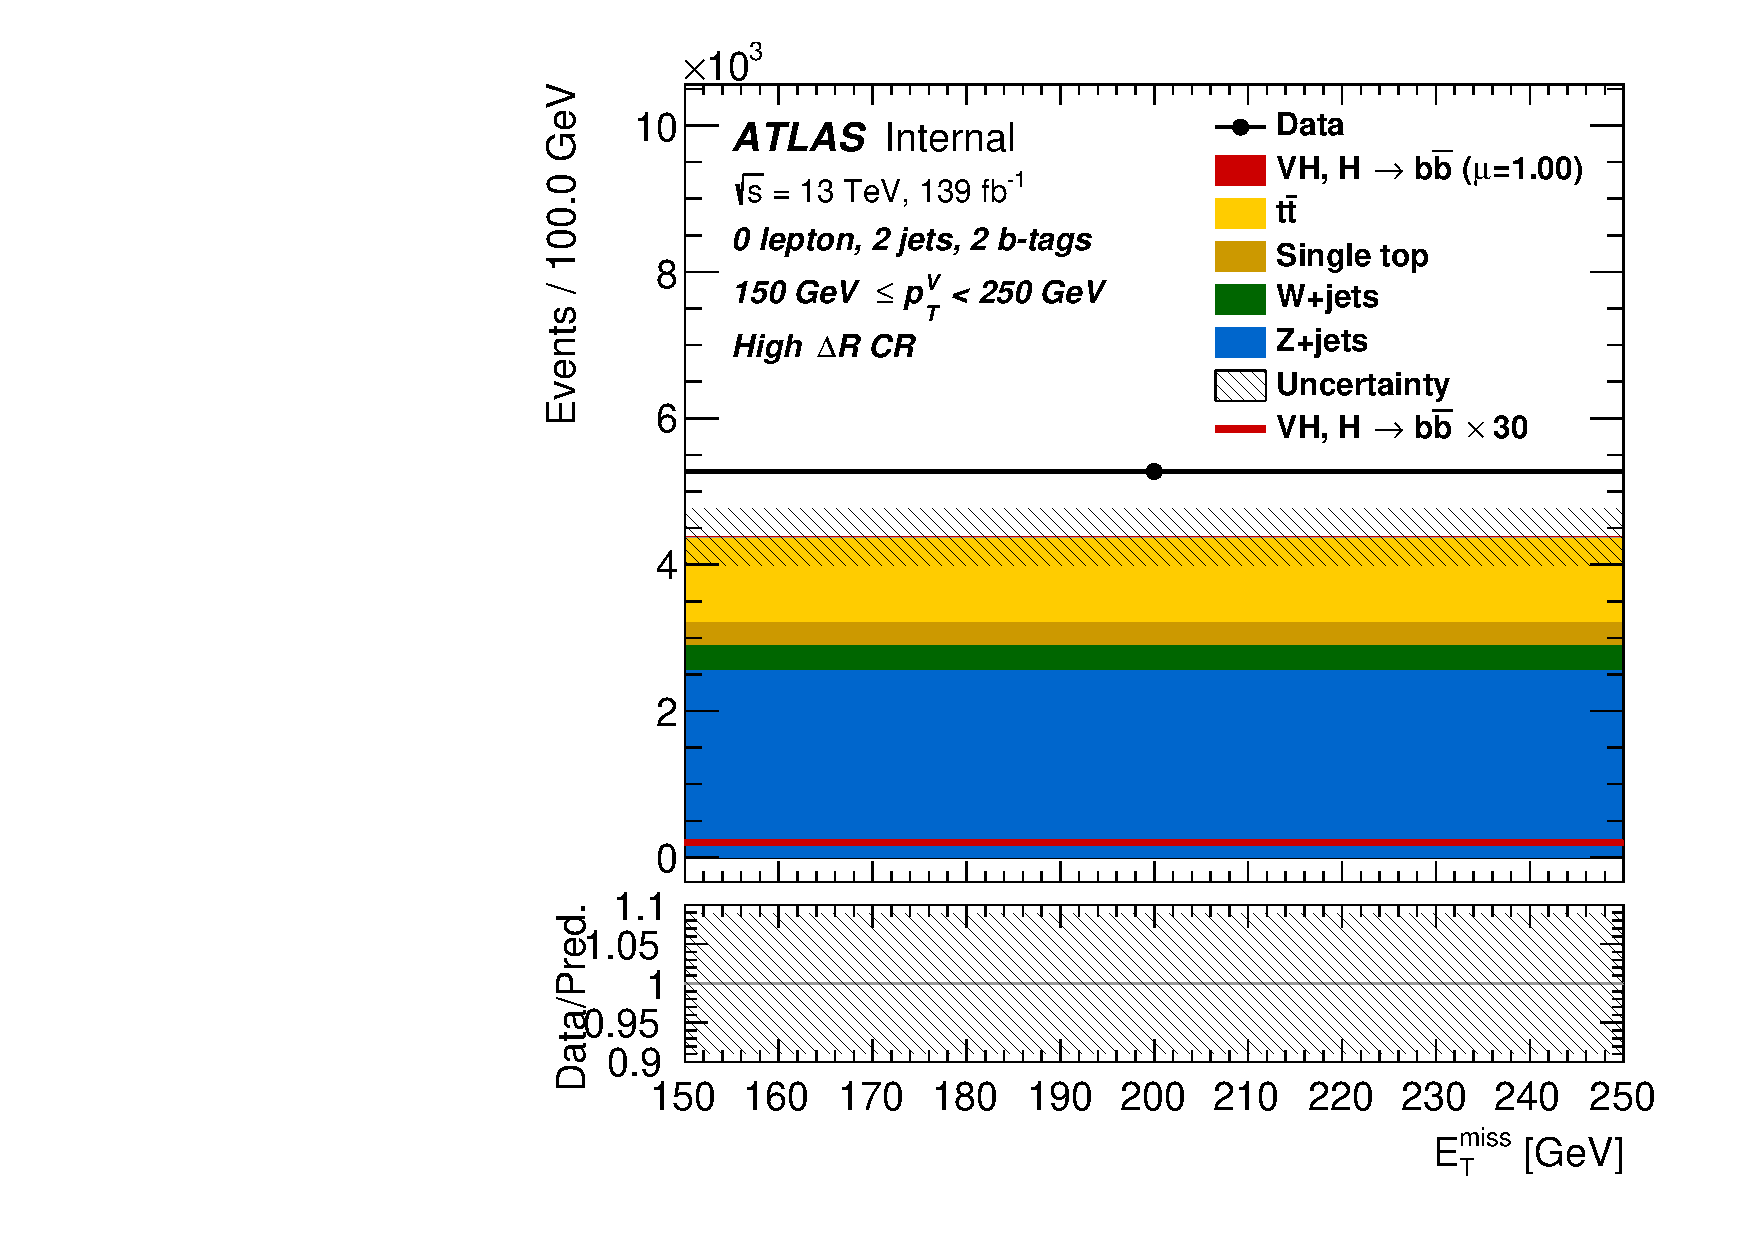
\includegraphics[width=.49\textwidth]{final_fit_mva/prefit/Region_BMax250_BMin150_Y6051_DCRHigh_T2_L0_distMET_J2_Prefit}%
    & 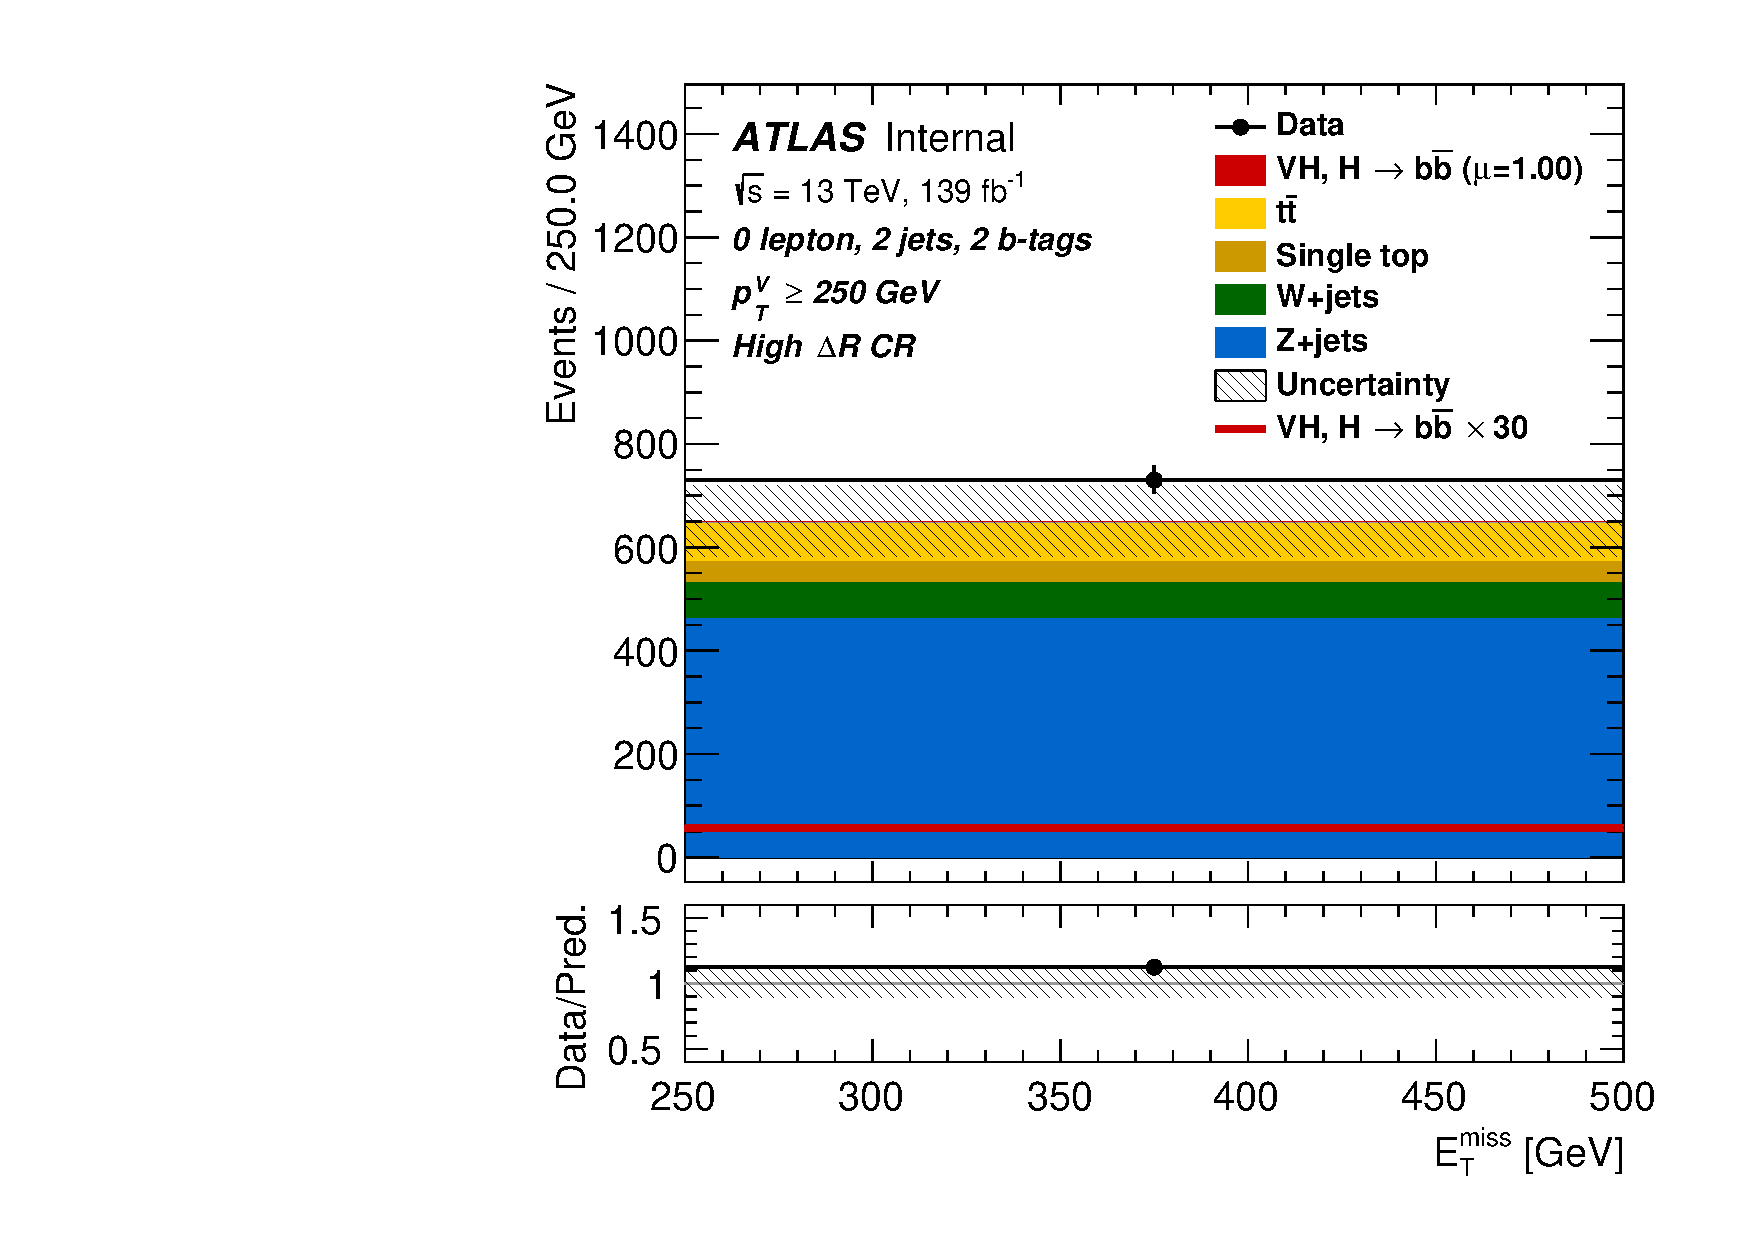
\includegraphics[width=.49\textwidth]{final_fit_mva/prefit/Region_BMin250_Y6051_DCRHigh_T2_L0_distMET_J2_Prefit} \\

    % middle row
    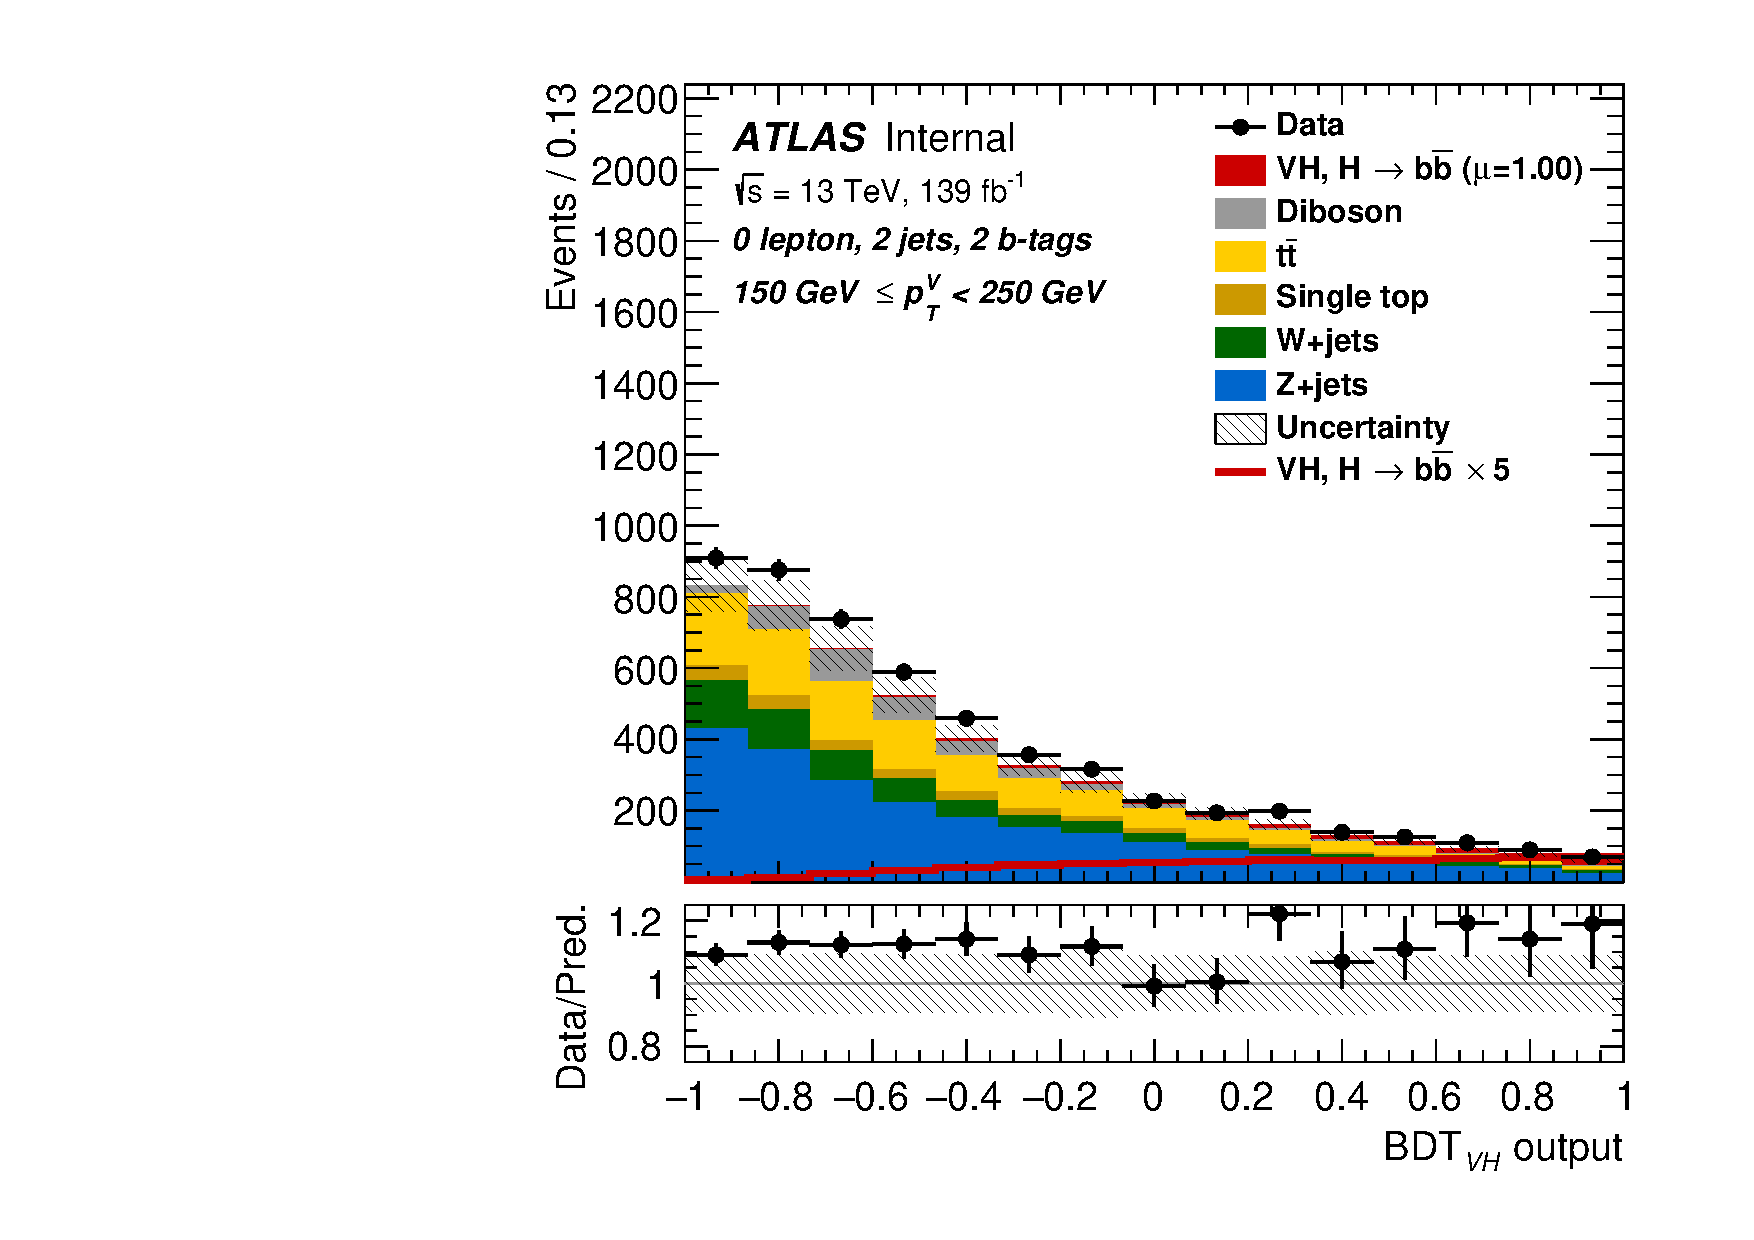
\includegraphics[width=.49\textwidth]{final_fit_mva/prefit/Region_BMax250_BMin150_Y6051_DSR_T2_L0_distmva_J2_Prefit}%
    & 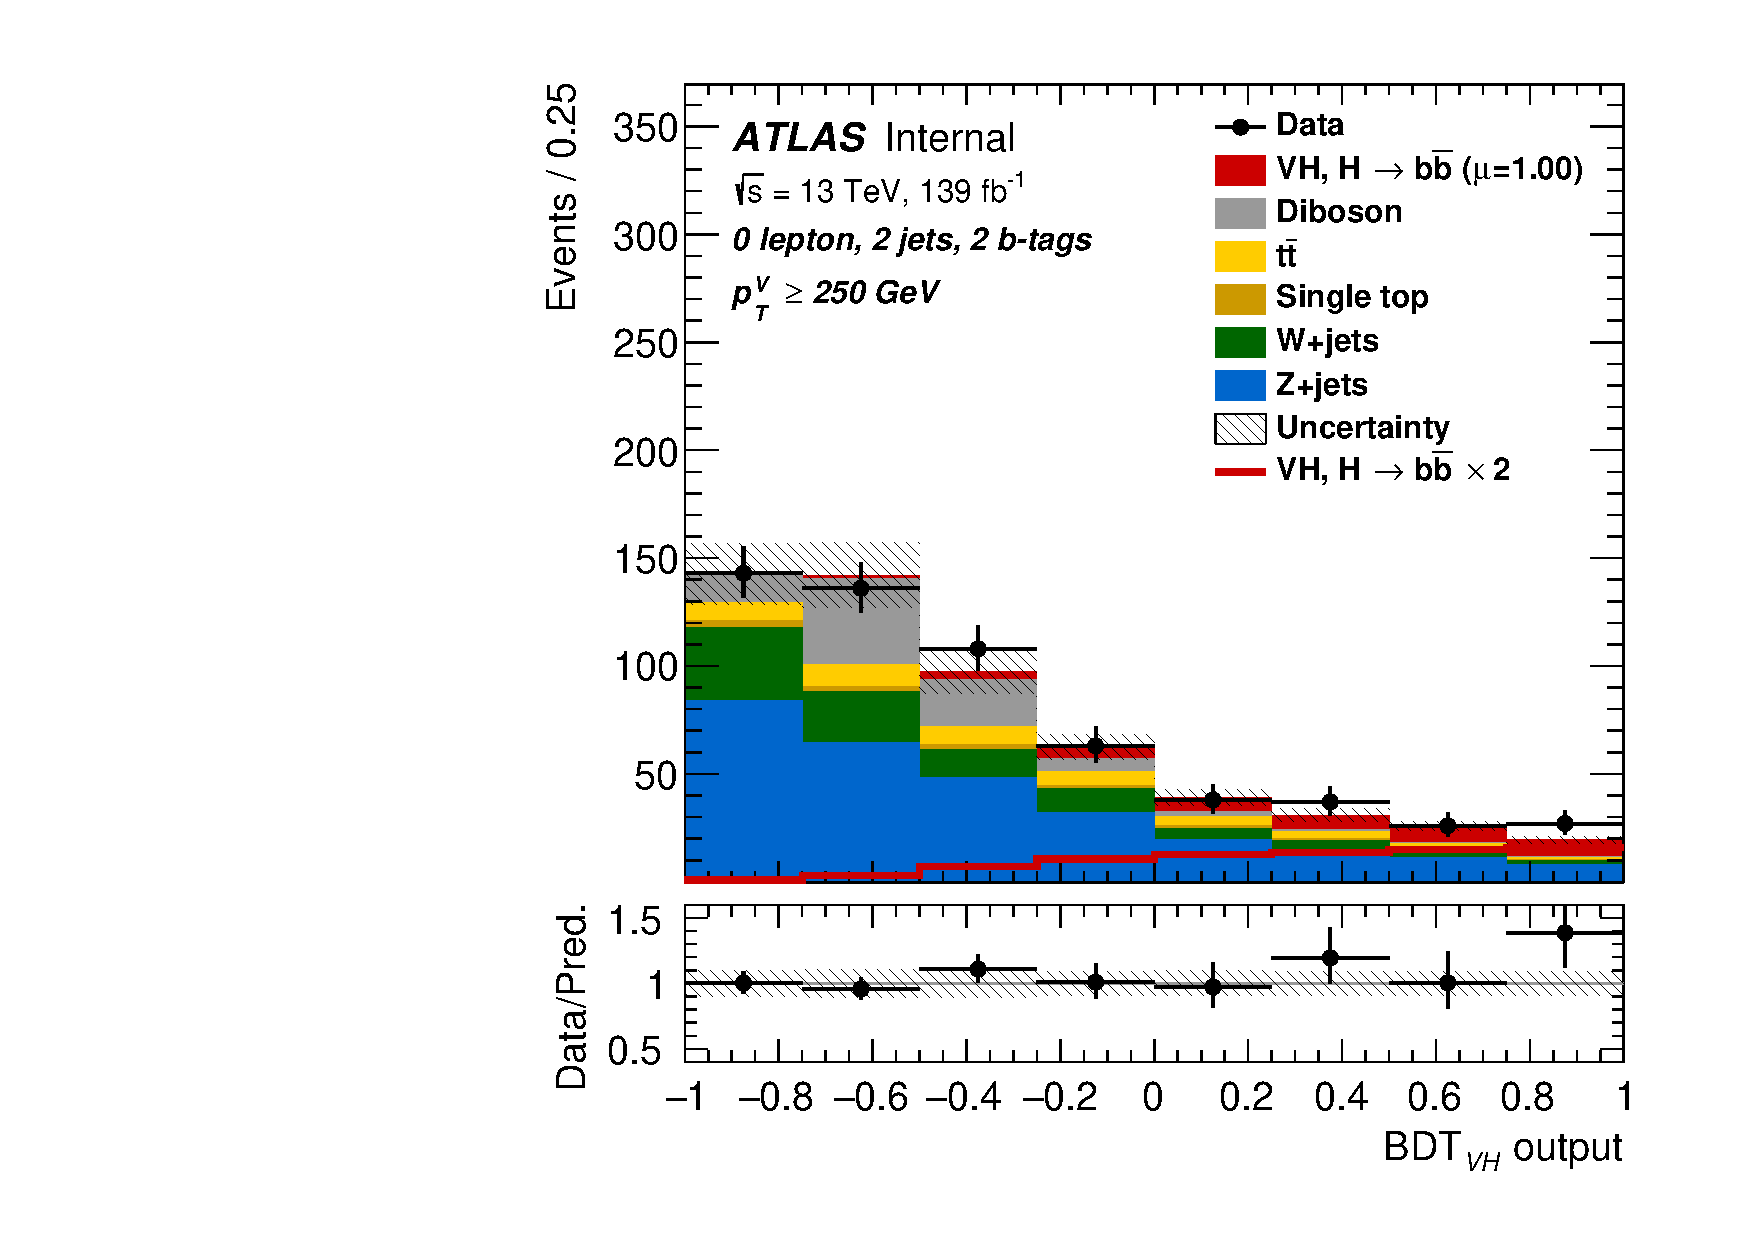
\includegraphics[width=.49\textwidth]{final_fit_mva/prefit/Region_BMin250_Y6051_DSR_T2_L0_distmva_J2_Prefit} \\

    % bottom row
    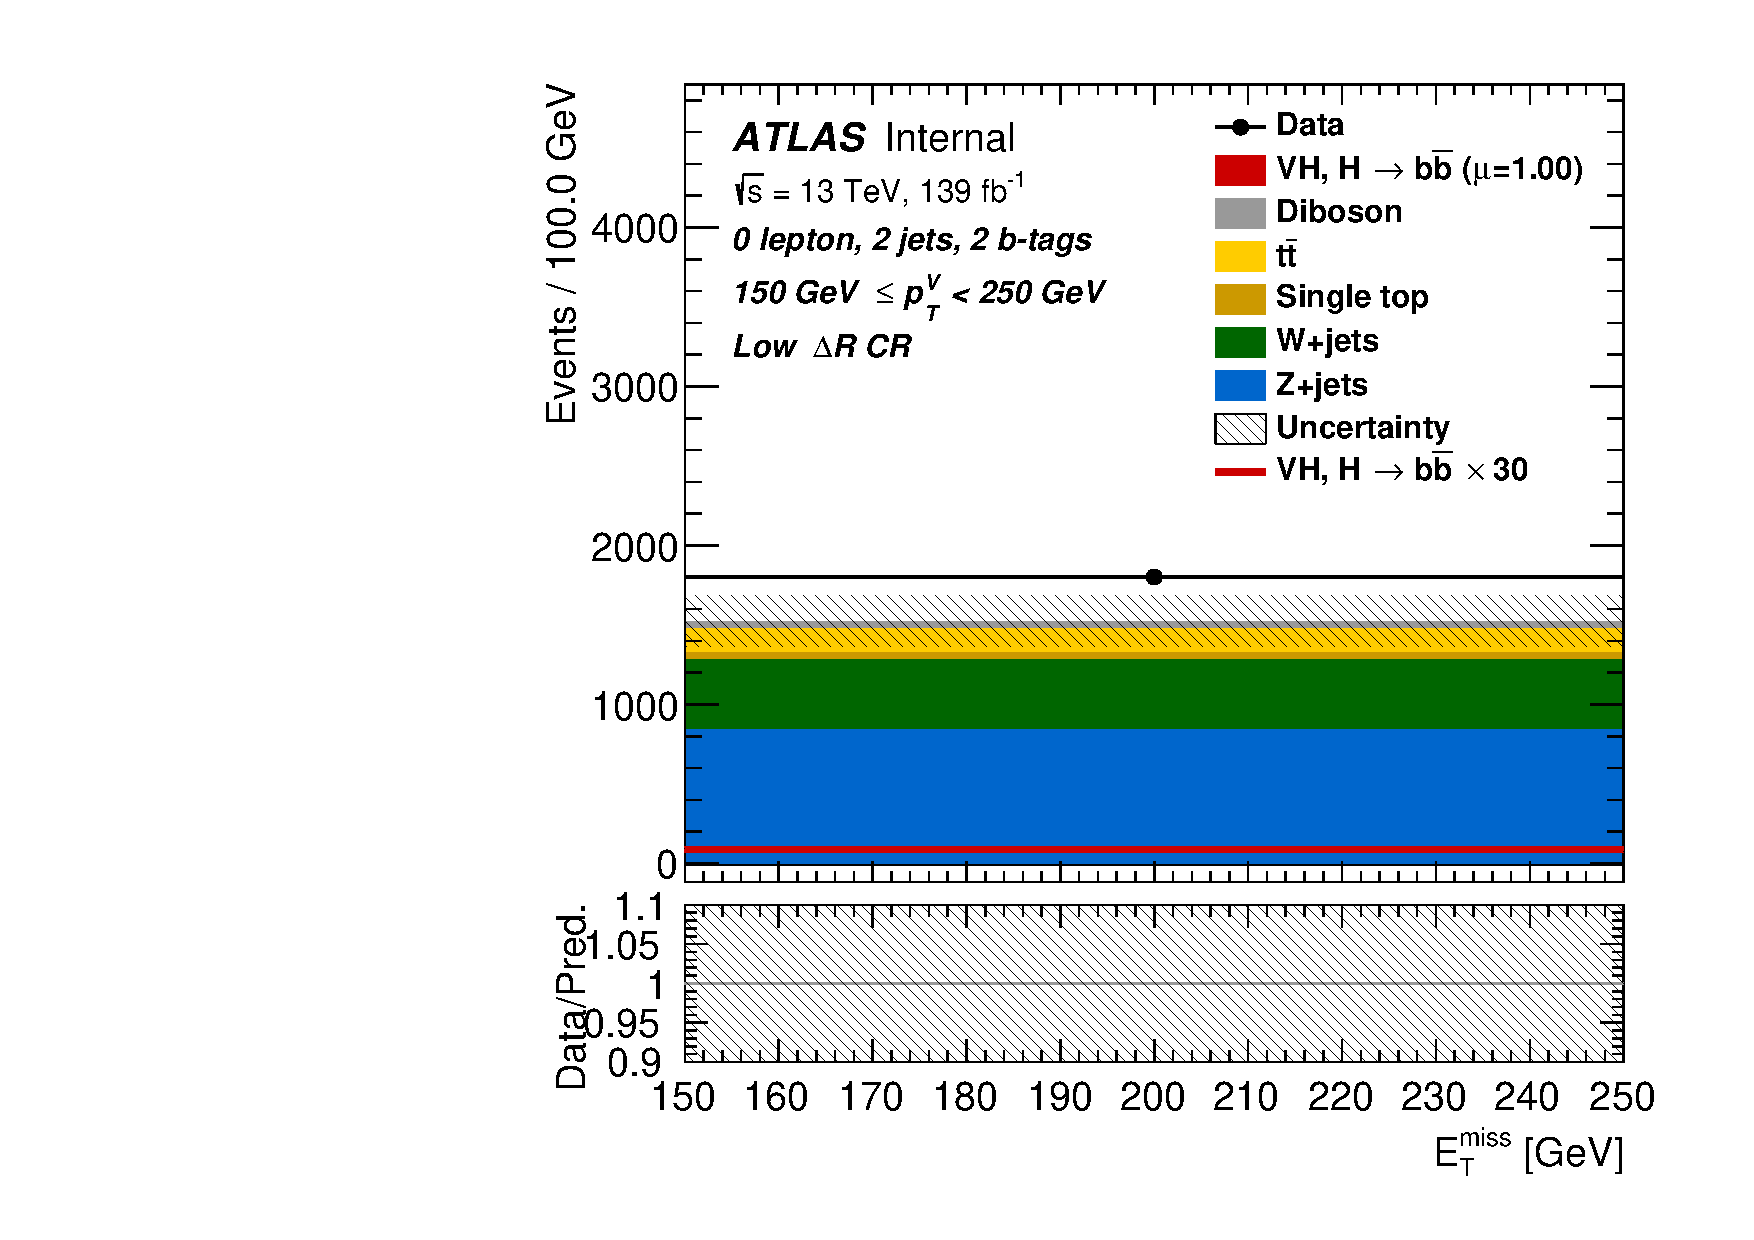
\includegraphics[width=.49\textwidth]{final_fit_mva/prefit/Region_BMax250_BMin150_Y6051_DCRLow_T2_L0_distMET_J2_Prefit}%
    & 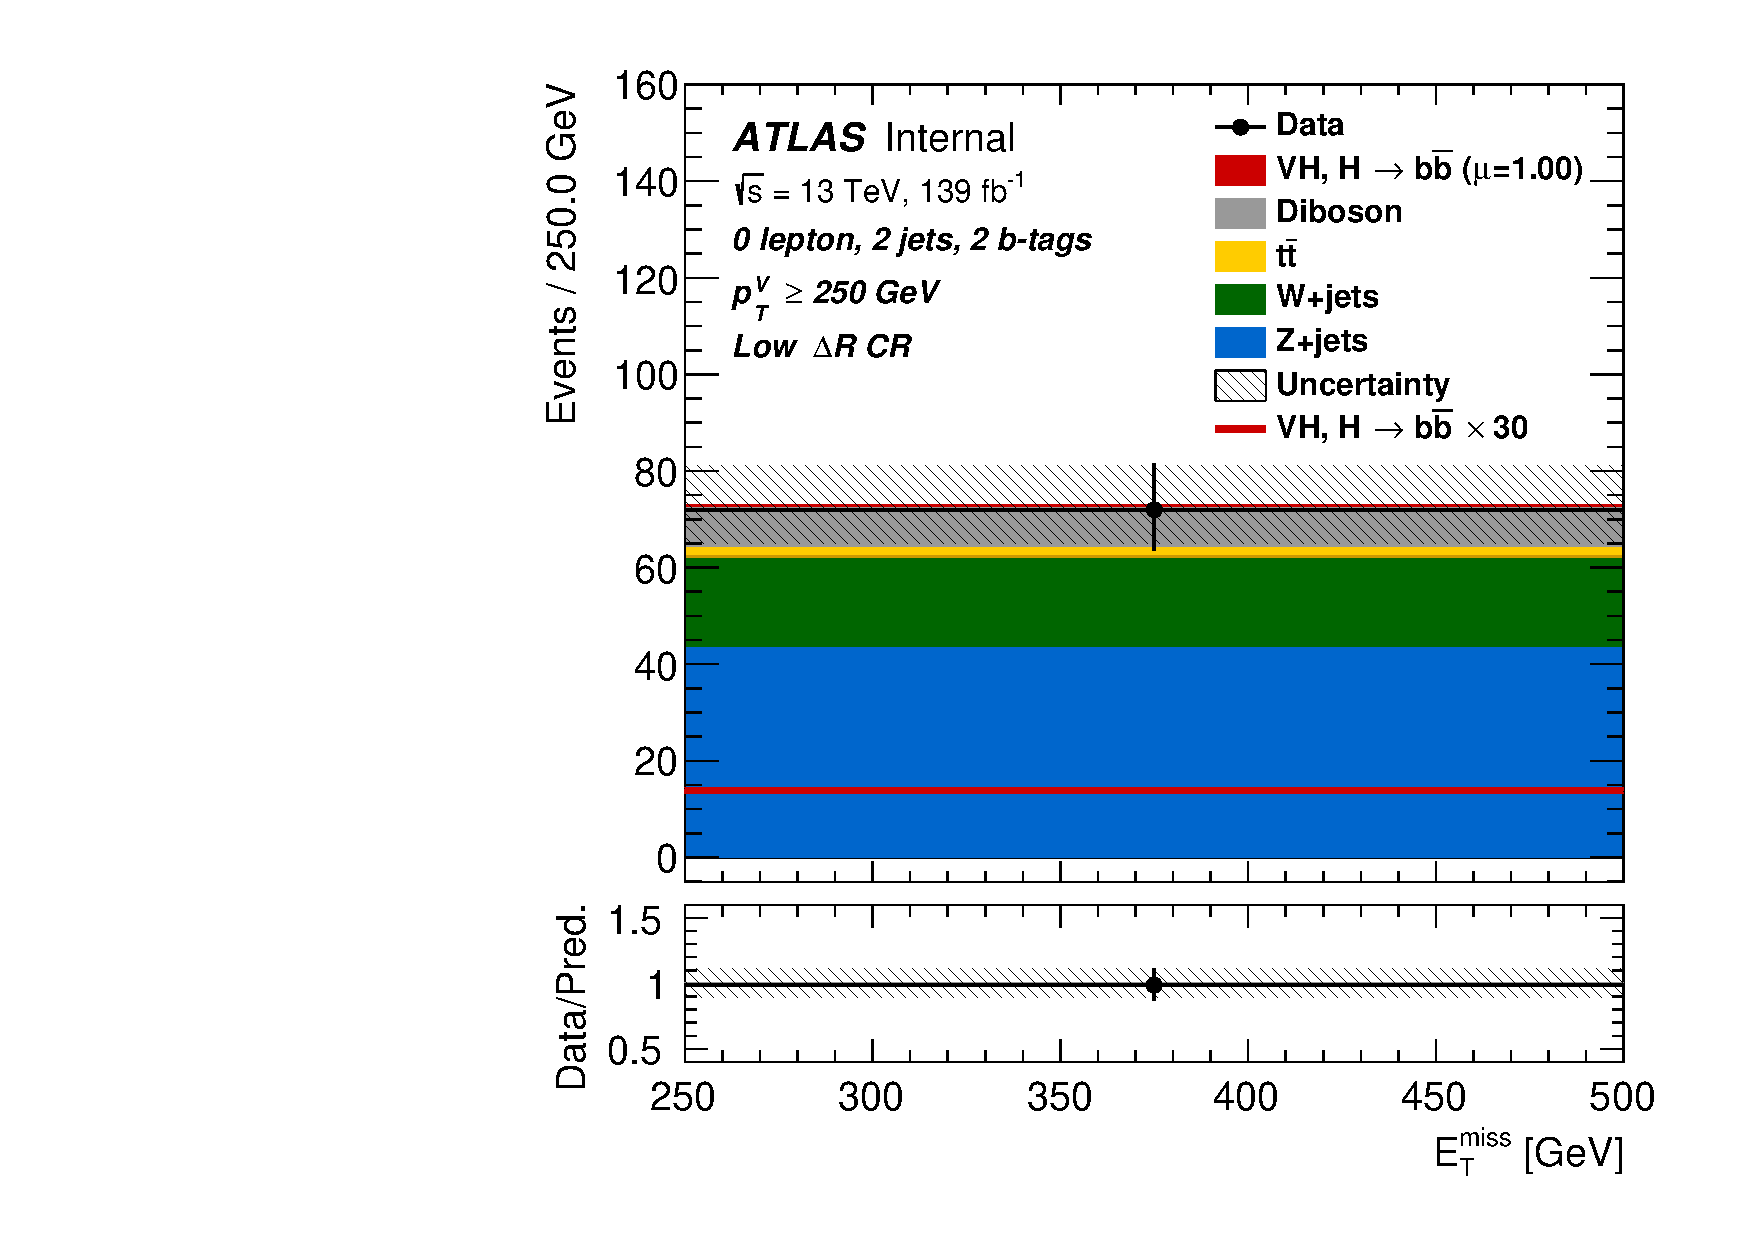
\includegraphics[width=.49\textwidth]{final_fit_mva/prefit/Region_BMin250_Y6051_DCRLow_T2_L0_distMET_J2_Prefit} \\
  \end{tabular}
  \caption{Pre-fit distributions in the 0--lepton channel in the 2--jet region.}
  \label{fig:0lep-2jet-prefit}
\end{figure}
\begin{figure}
  \centering
  \begin{tabular}{cc}
    % top row
    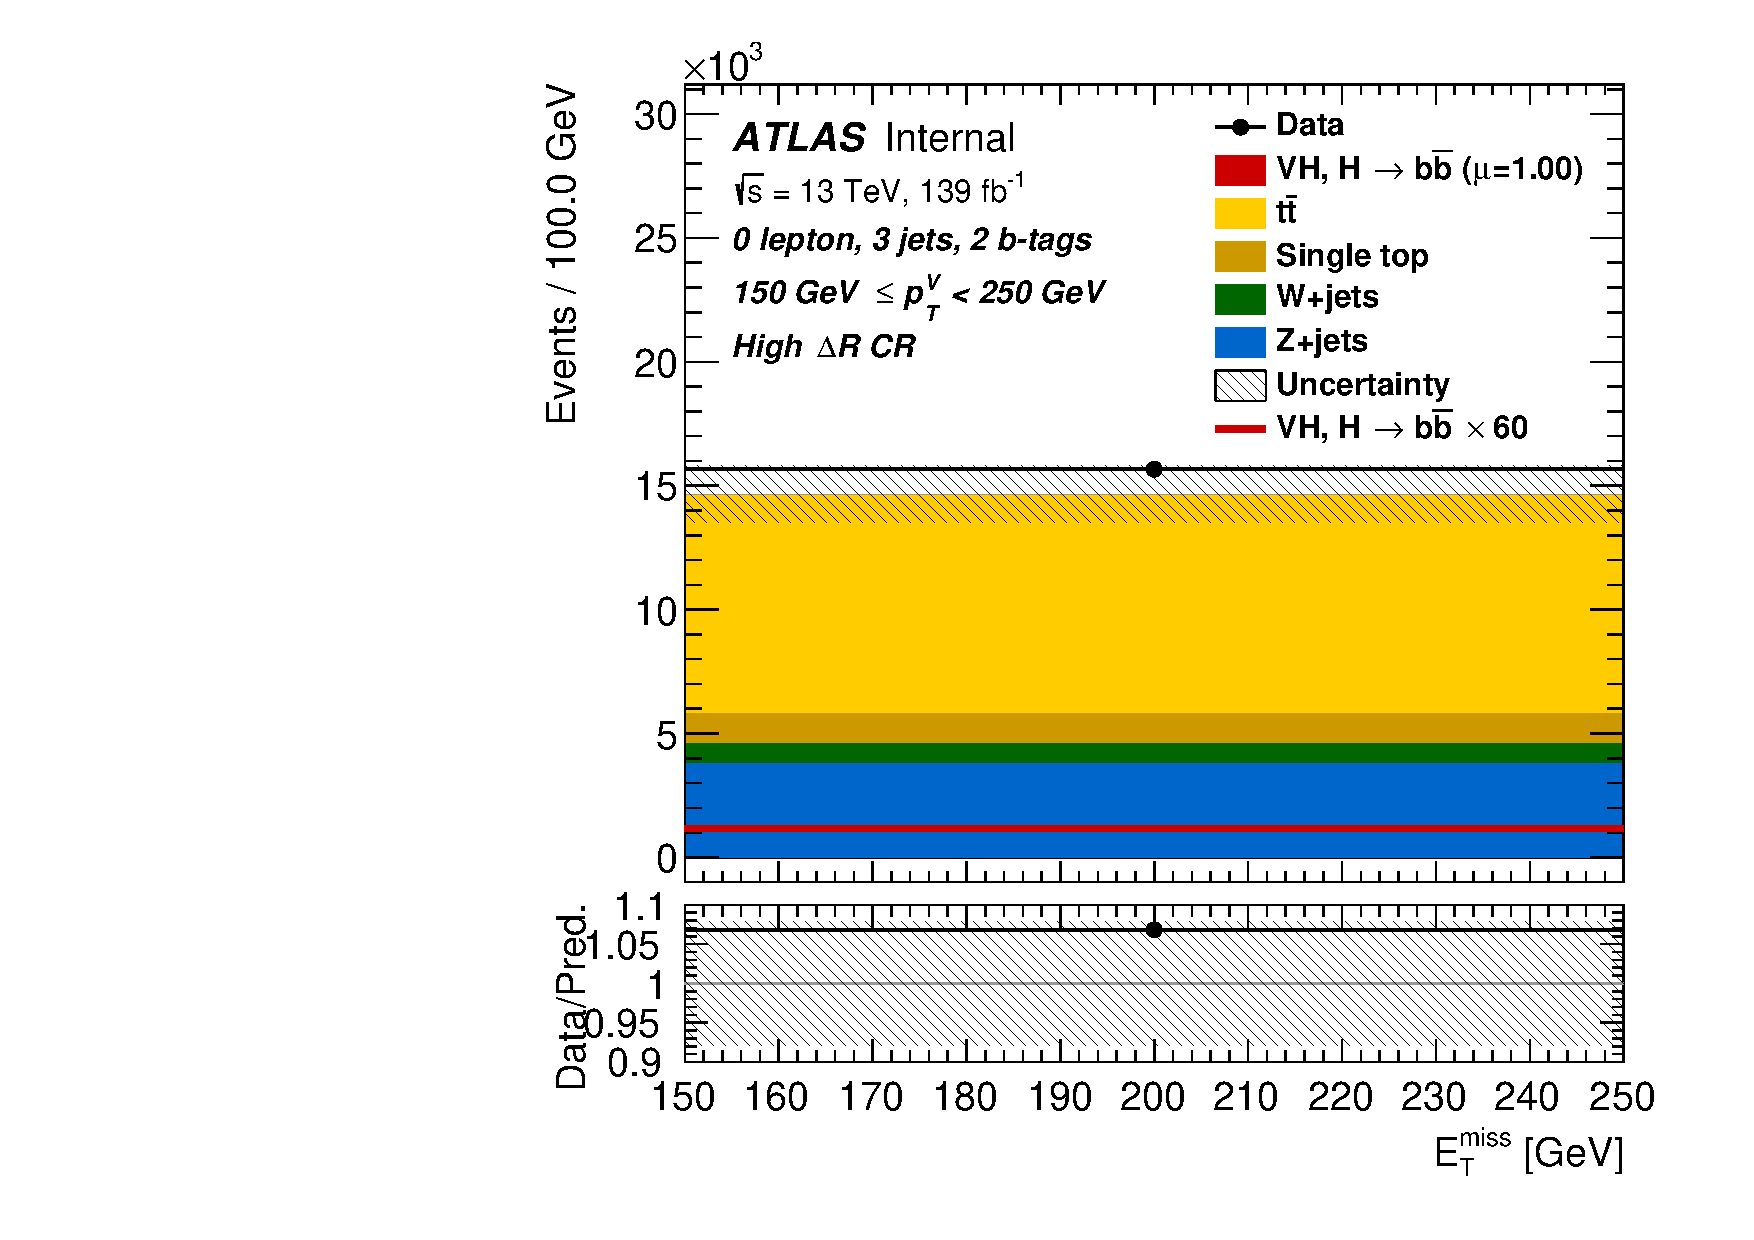
\includegraphics[width=.3\textwidth]{final_fit_mva/prefit/Region_BMax250_BMin150_Y6051_DCRHigh_T2_L0_distMET_J3_Prefit}%
    & 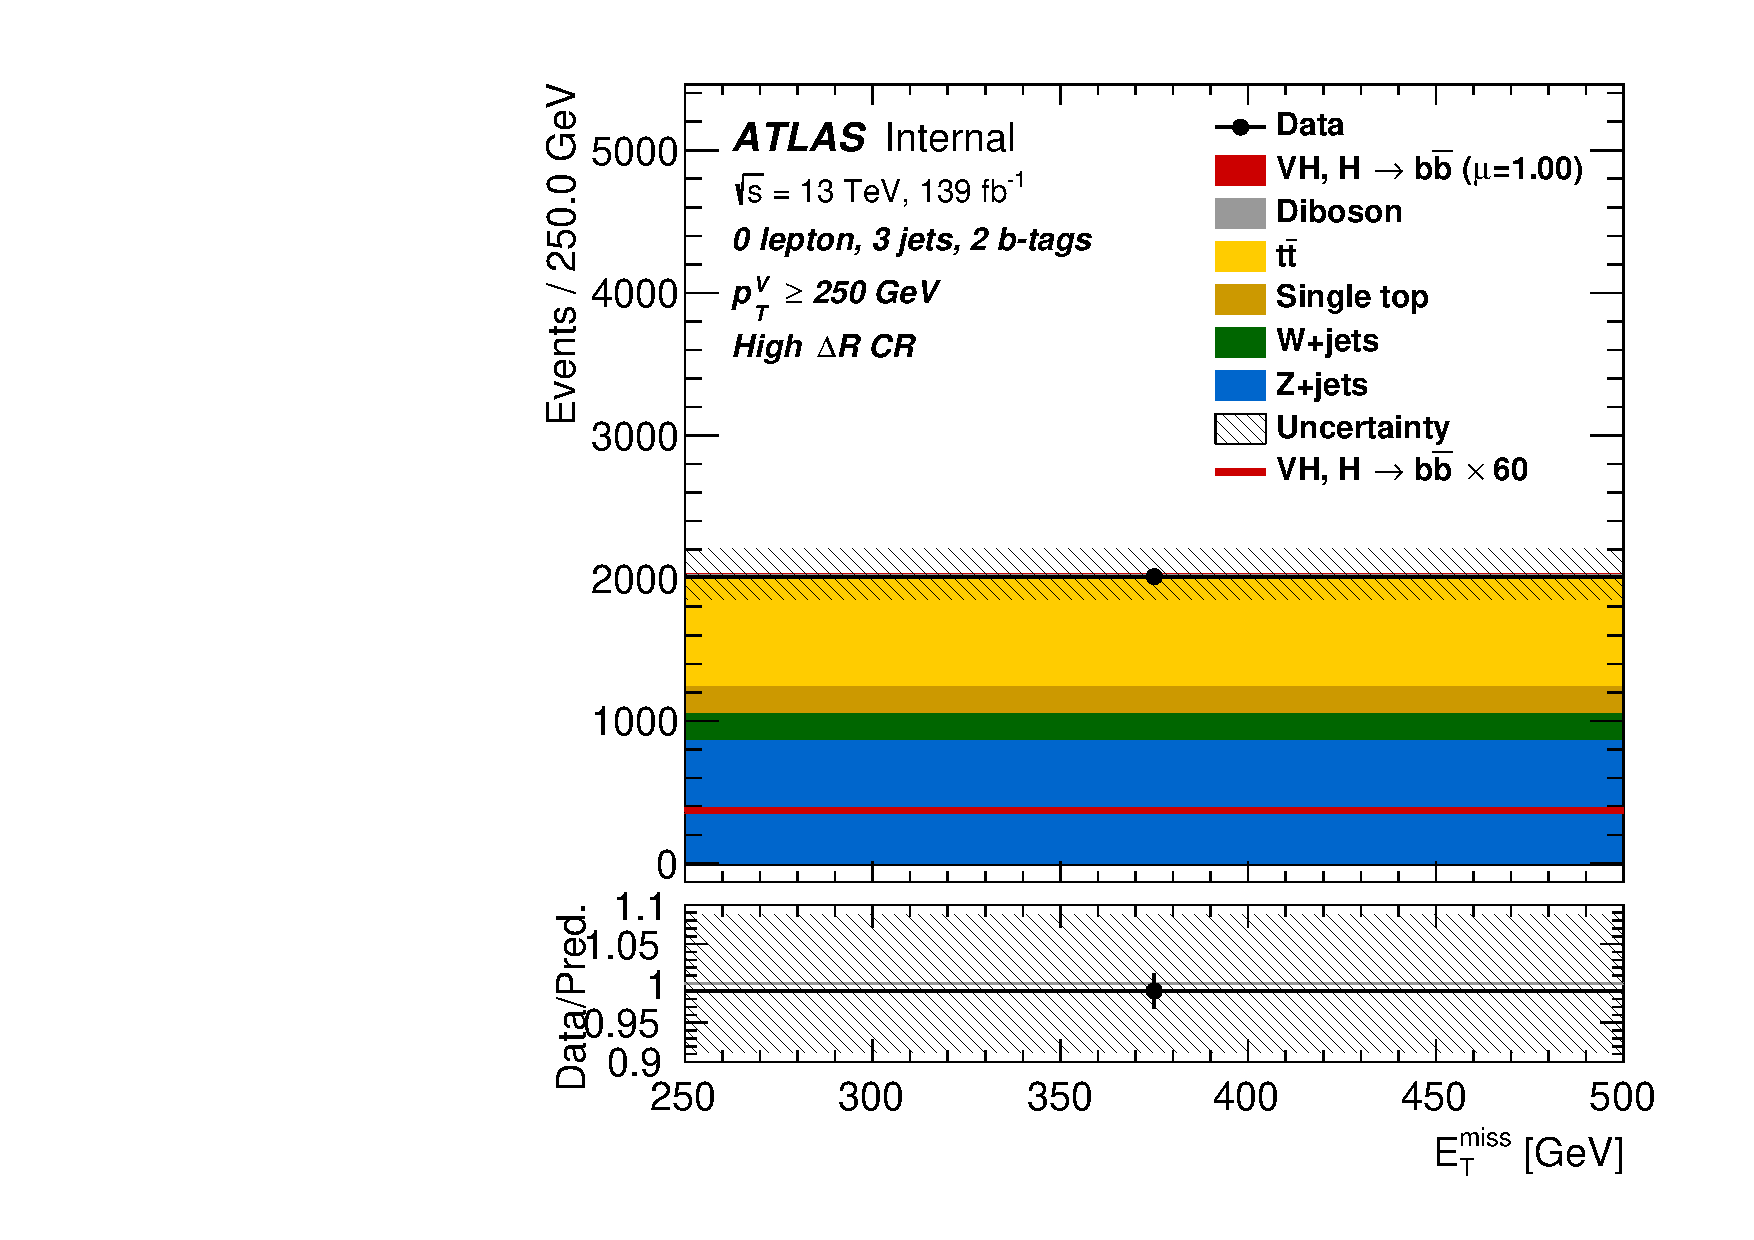
\includegraphics[width=.3\textwidth]{final_fit_mva/prefit/Region_BMin250_Y6051_DCRHigh_T2_L0_distMET_J3_Prefit} \\

    % middle row
    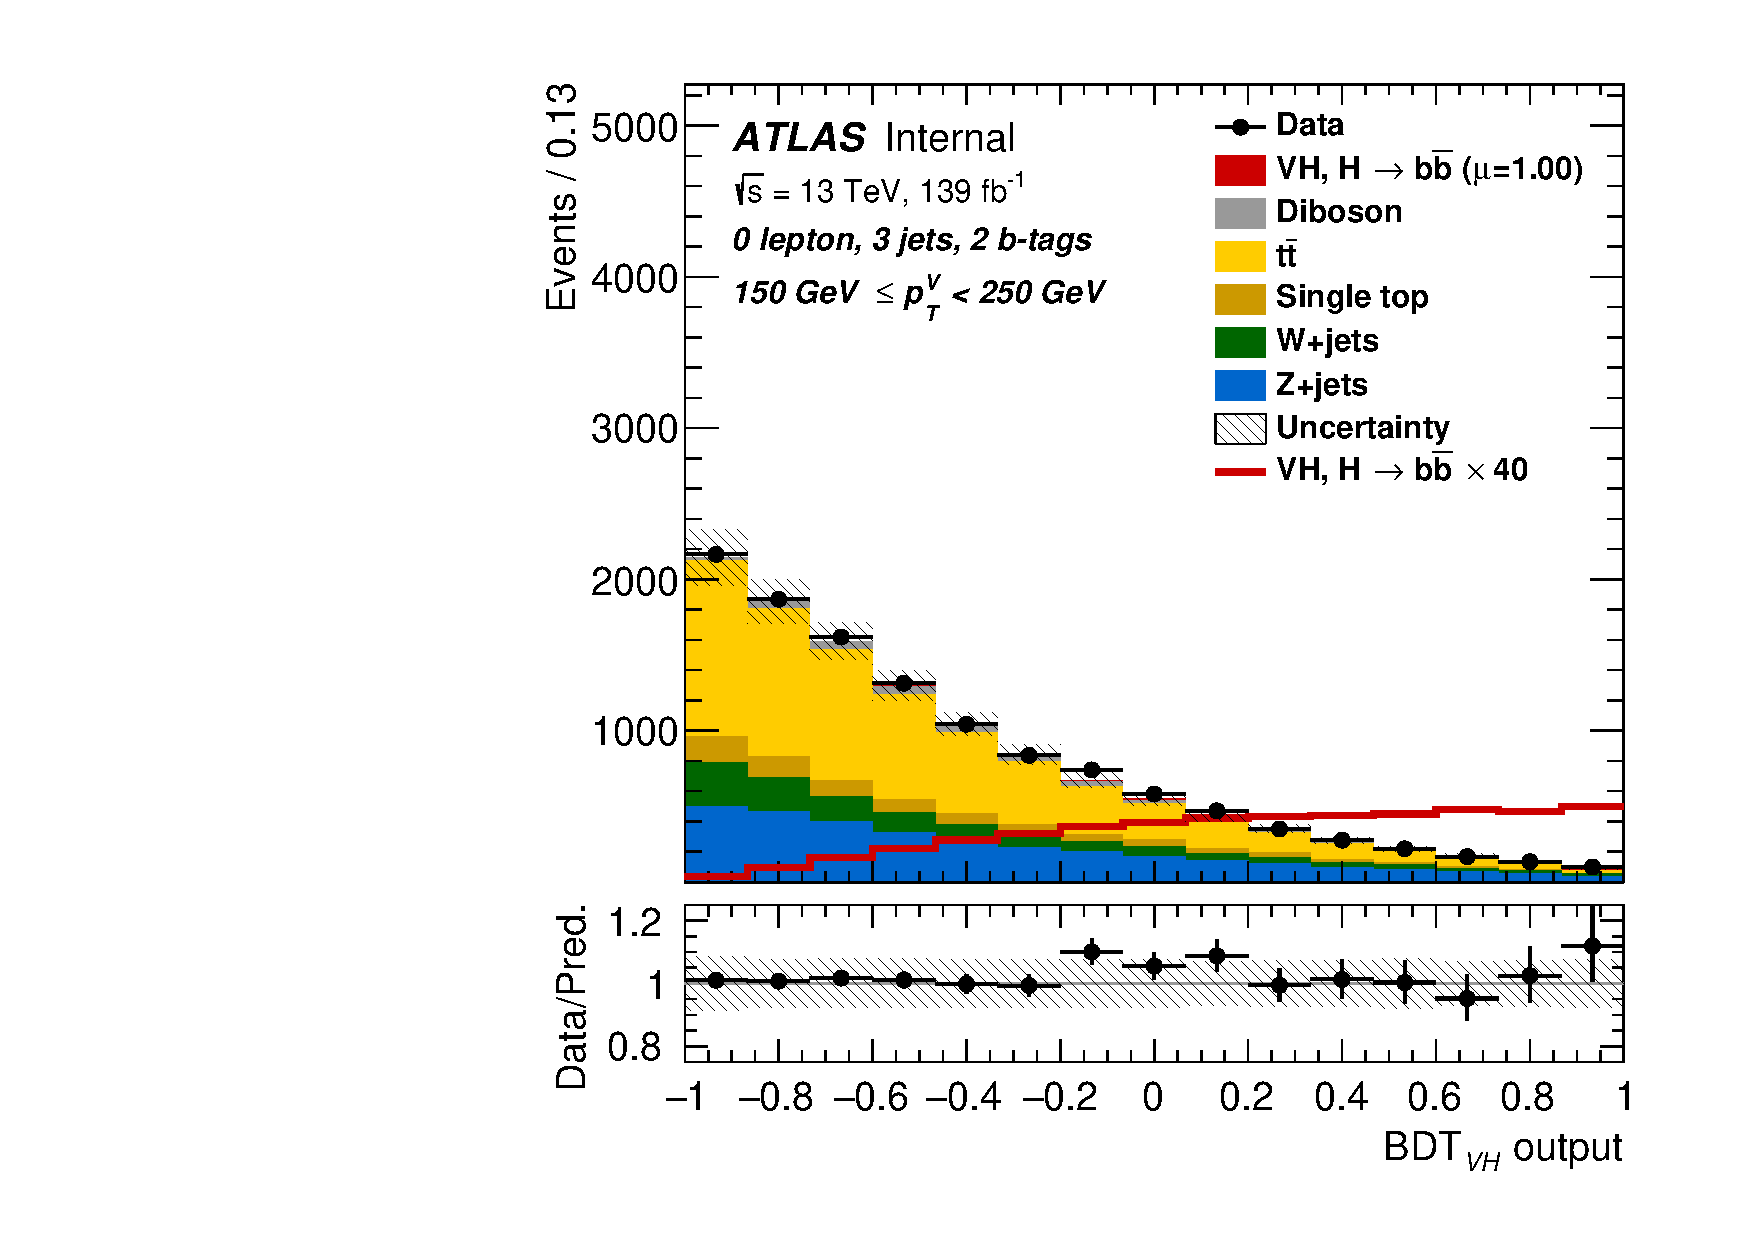
\includegraphics[width=.3\textwidth]{final_fit_mva/prefit/Region_BMax250_BMin150_Y6051_DSR_T2_L0_distmva_J3_Prefit}%
    & 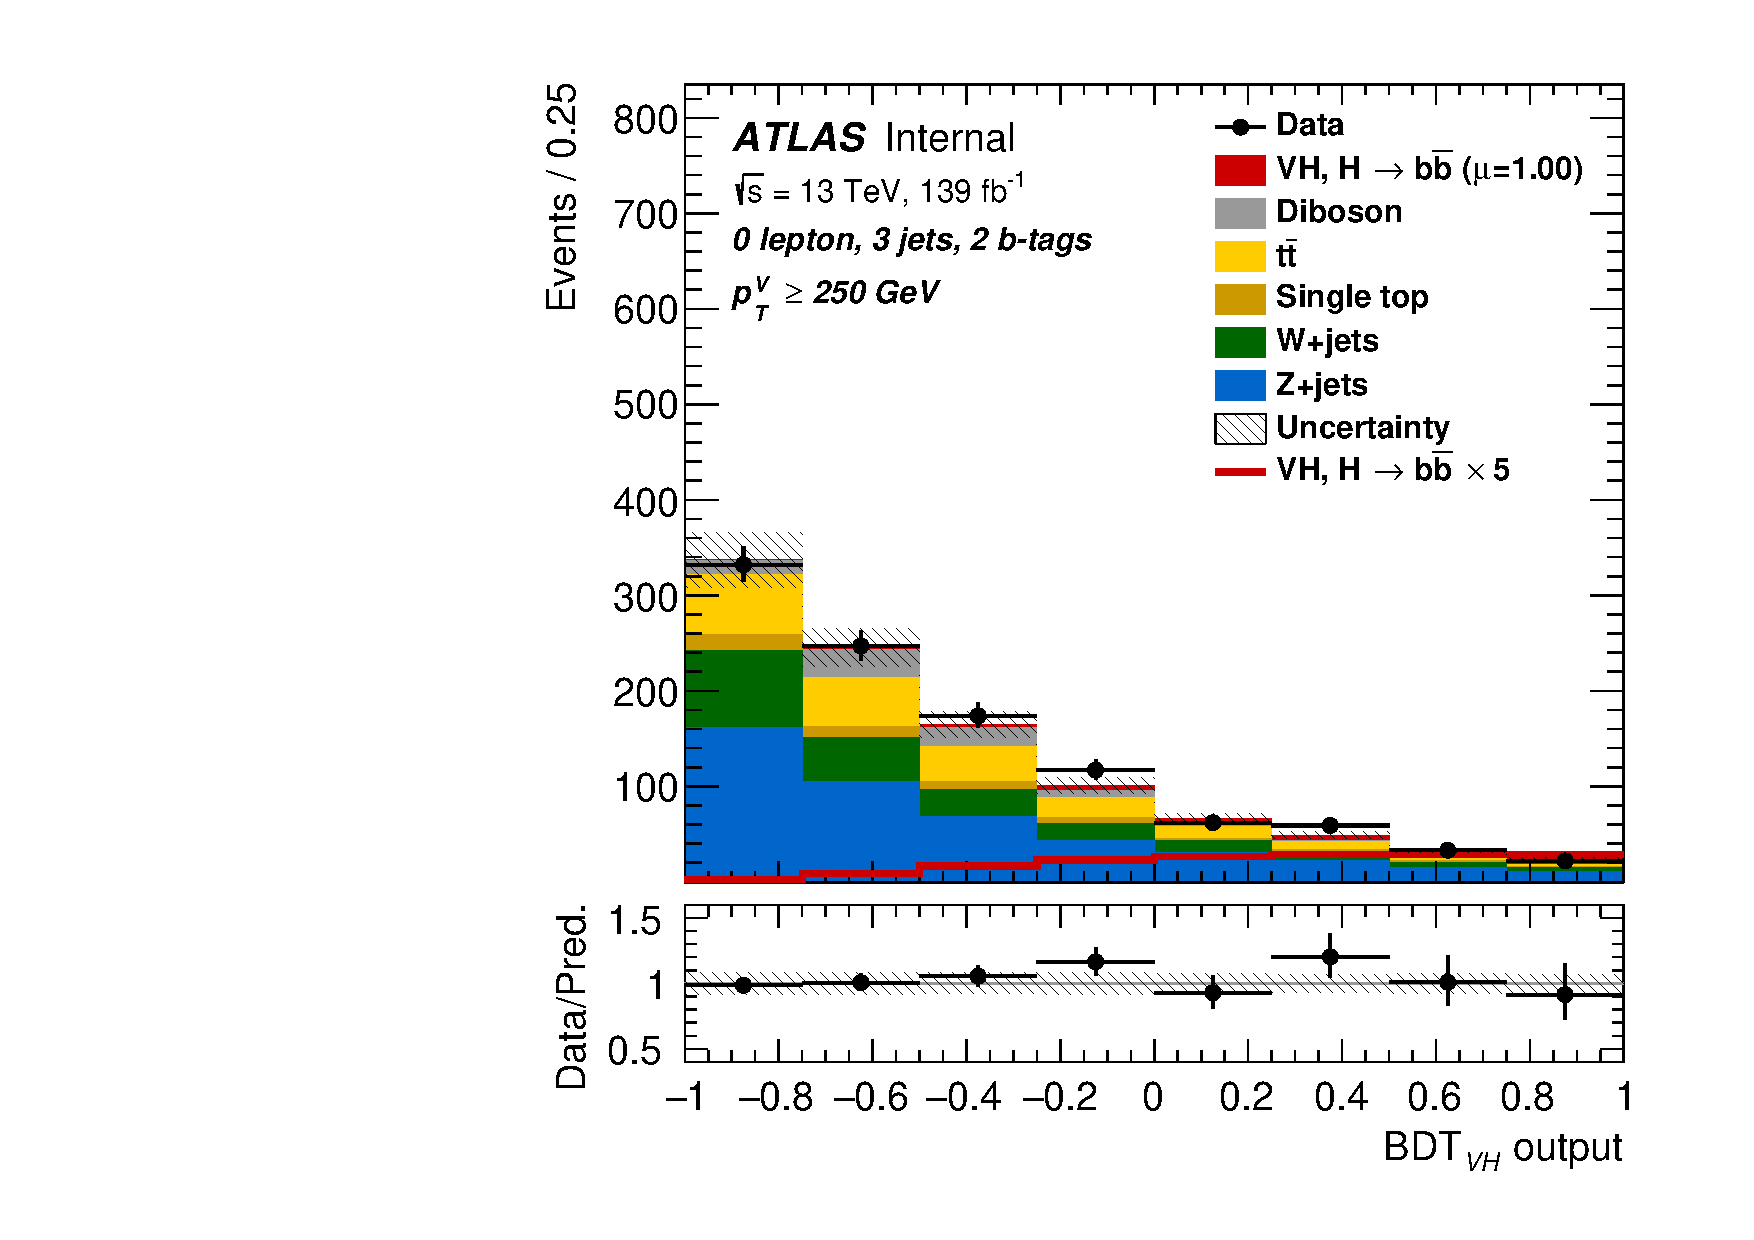
\includegraphics[width=.3\textwidth]{final_fit_mva/prefit/Region_BMin250_Y6051_DSR_T2_L0_distmva_J3_Prefit} \\

    % bottom row
    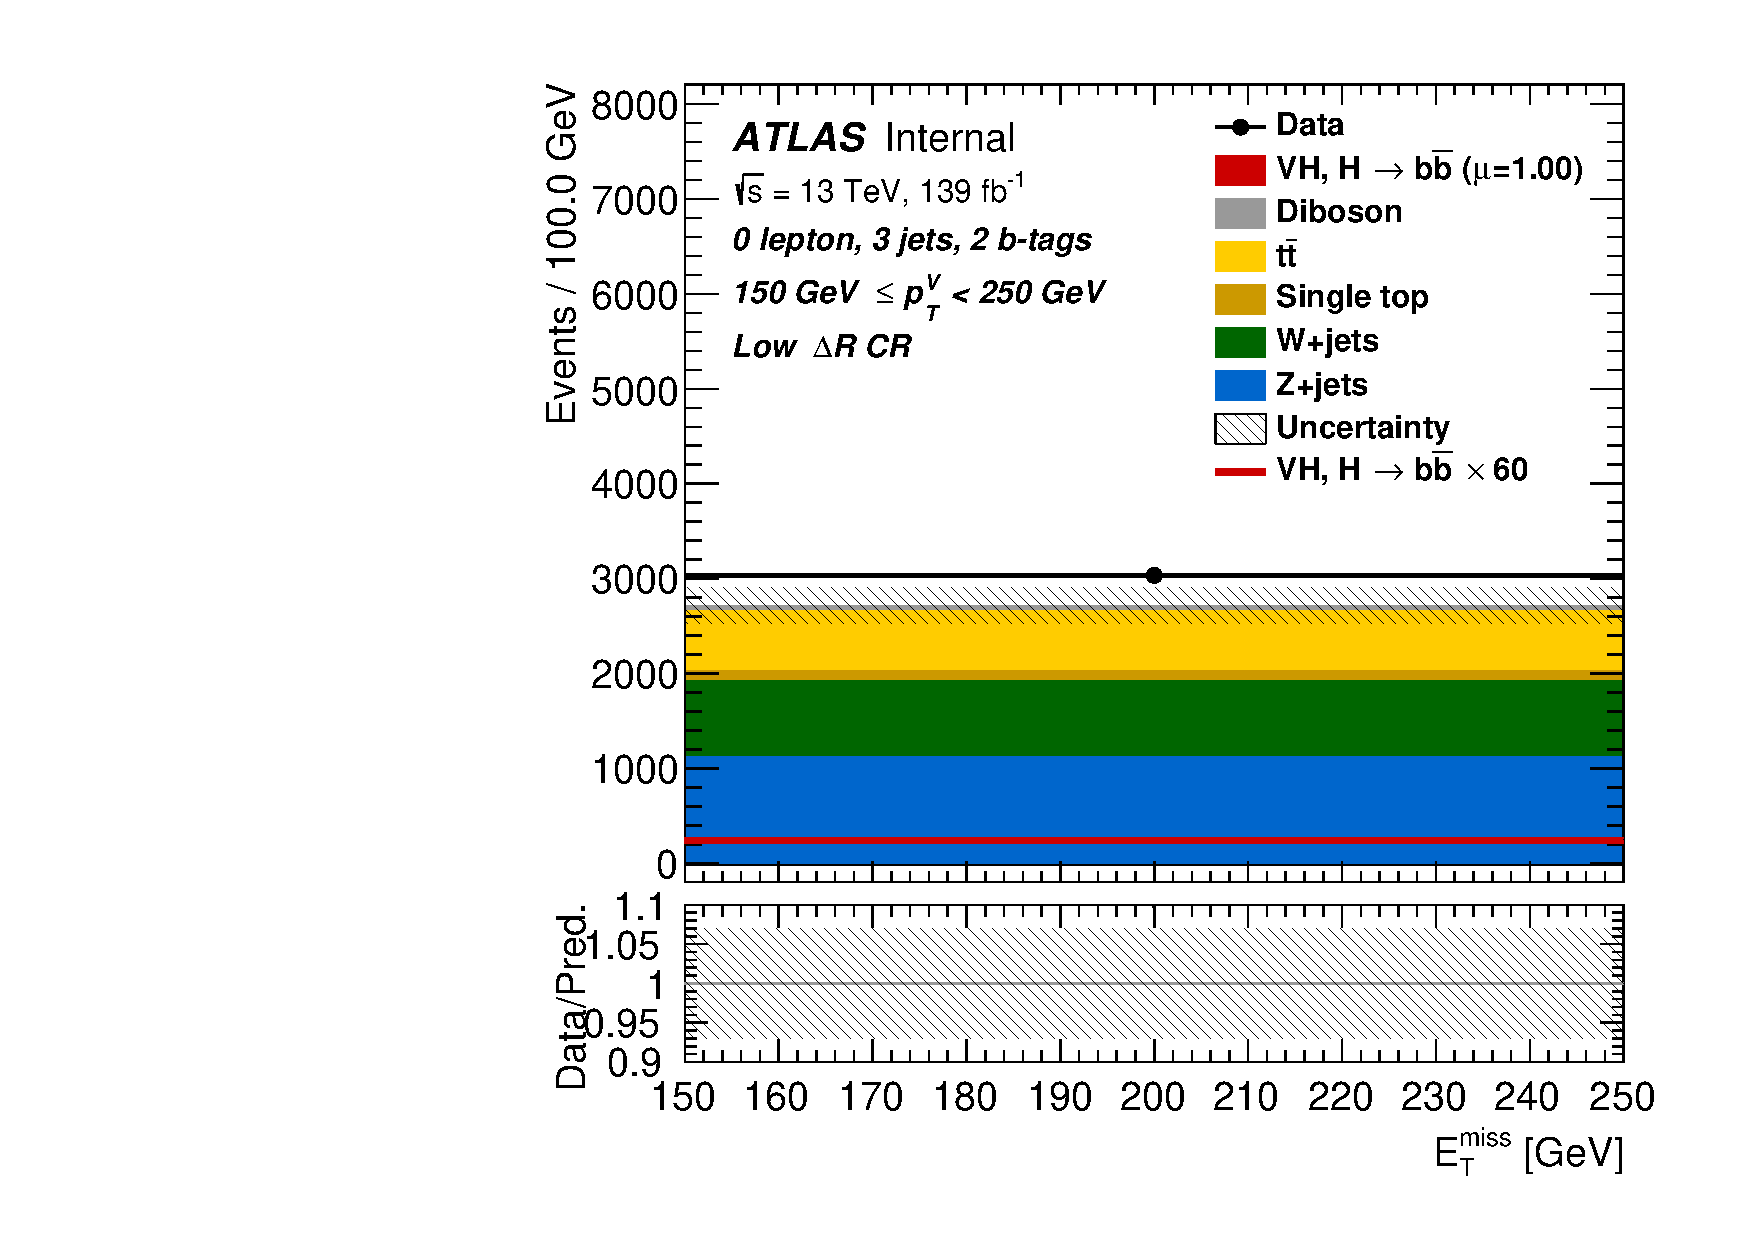
\includegraphics[width=.3\textwidth]{final_fit_mva/prefit/Region_BMax250_BMin150_Y6051_DCRLow_T2_L0_distMET_J3_Prefit}%
    & 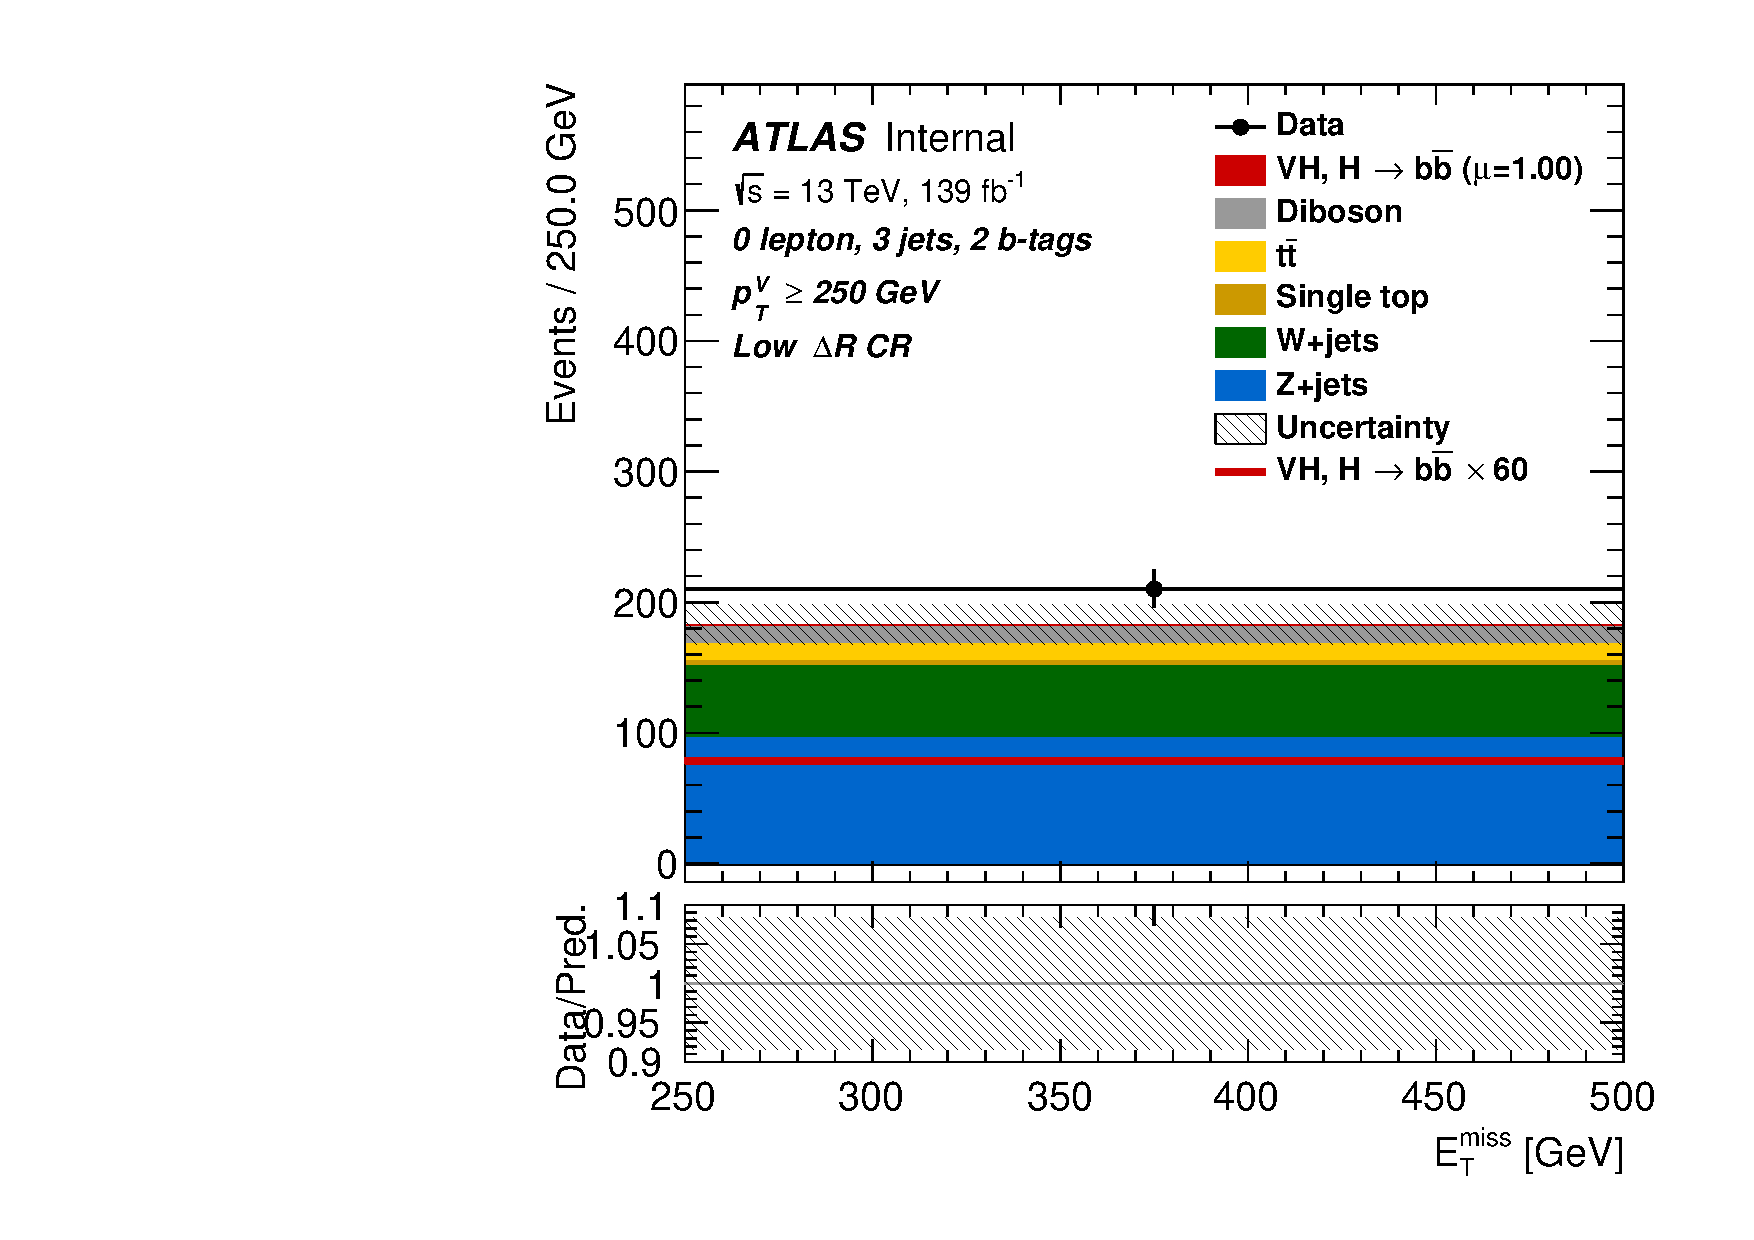
\includegraphics[width=.3\textwidth]{final_fit_mva/prefit/Region_BMin250_Y6051_DCRLow_T2_L0_distMET_J3_Prefit} \\
  \end{tabular}
  \caption{Pre-fit distributions in the 0 lepton 3 jet channel.}
\end{figure}
\begin{figure}
  \centering
  \begin{tabular}{cc}
    % top row
    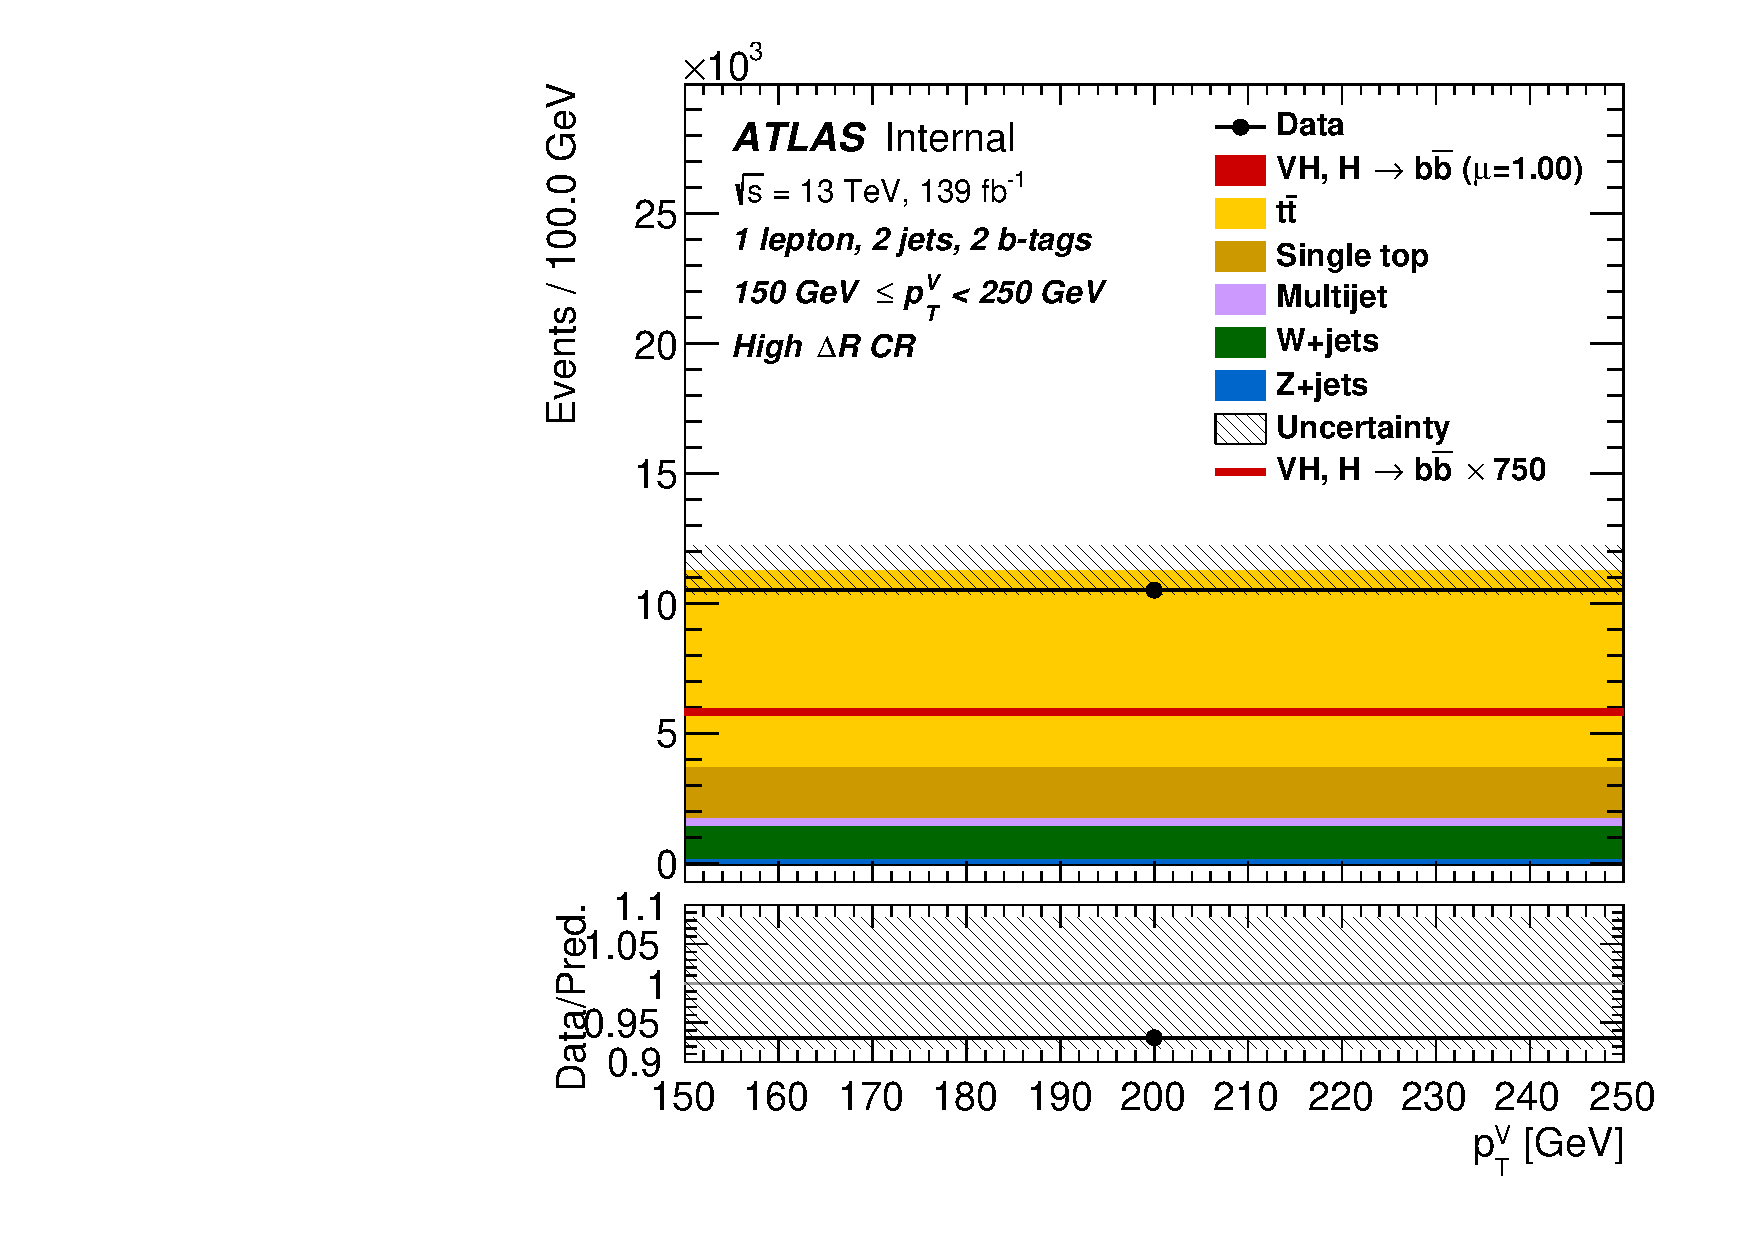
\includegraphics[width=.3\textwidth]{final_fit_mva/prefit/Region_BMax250_BMin150_Y6051_DCRHigh_T2_L1_distpTV_J2_Prefit}%
    & 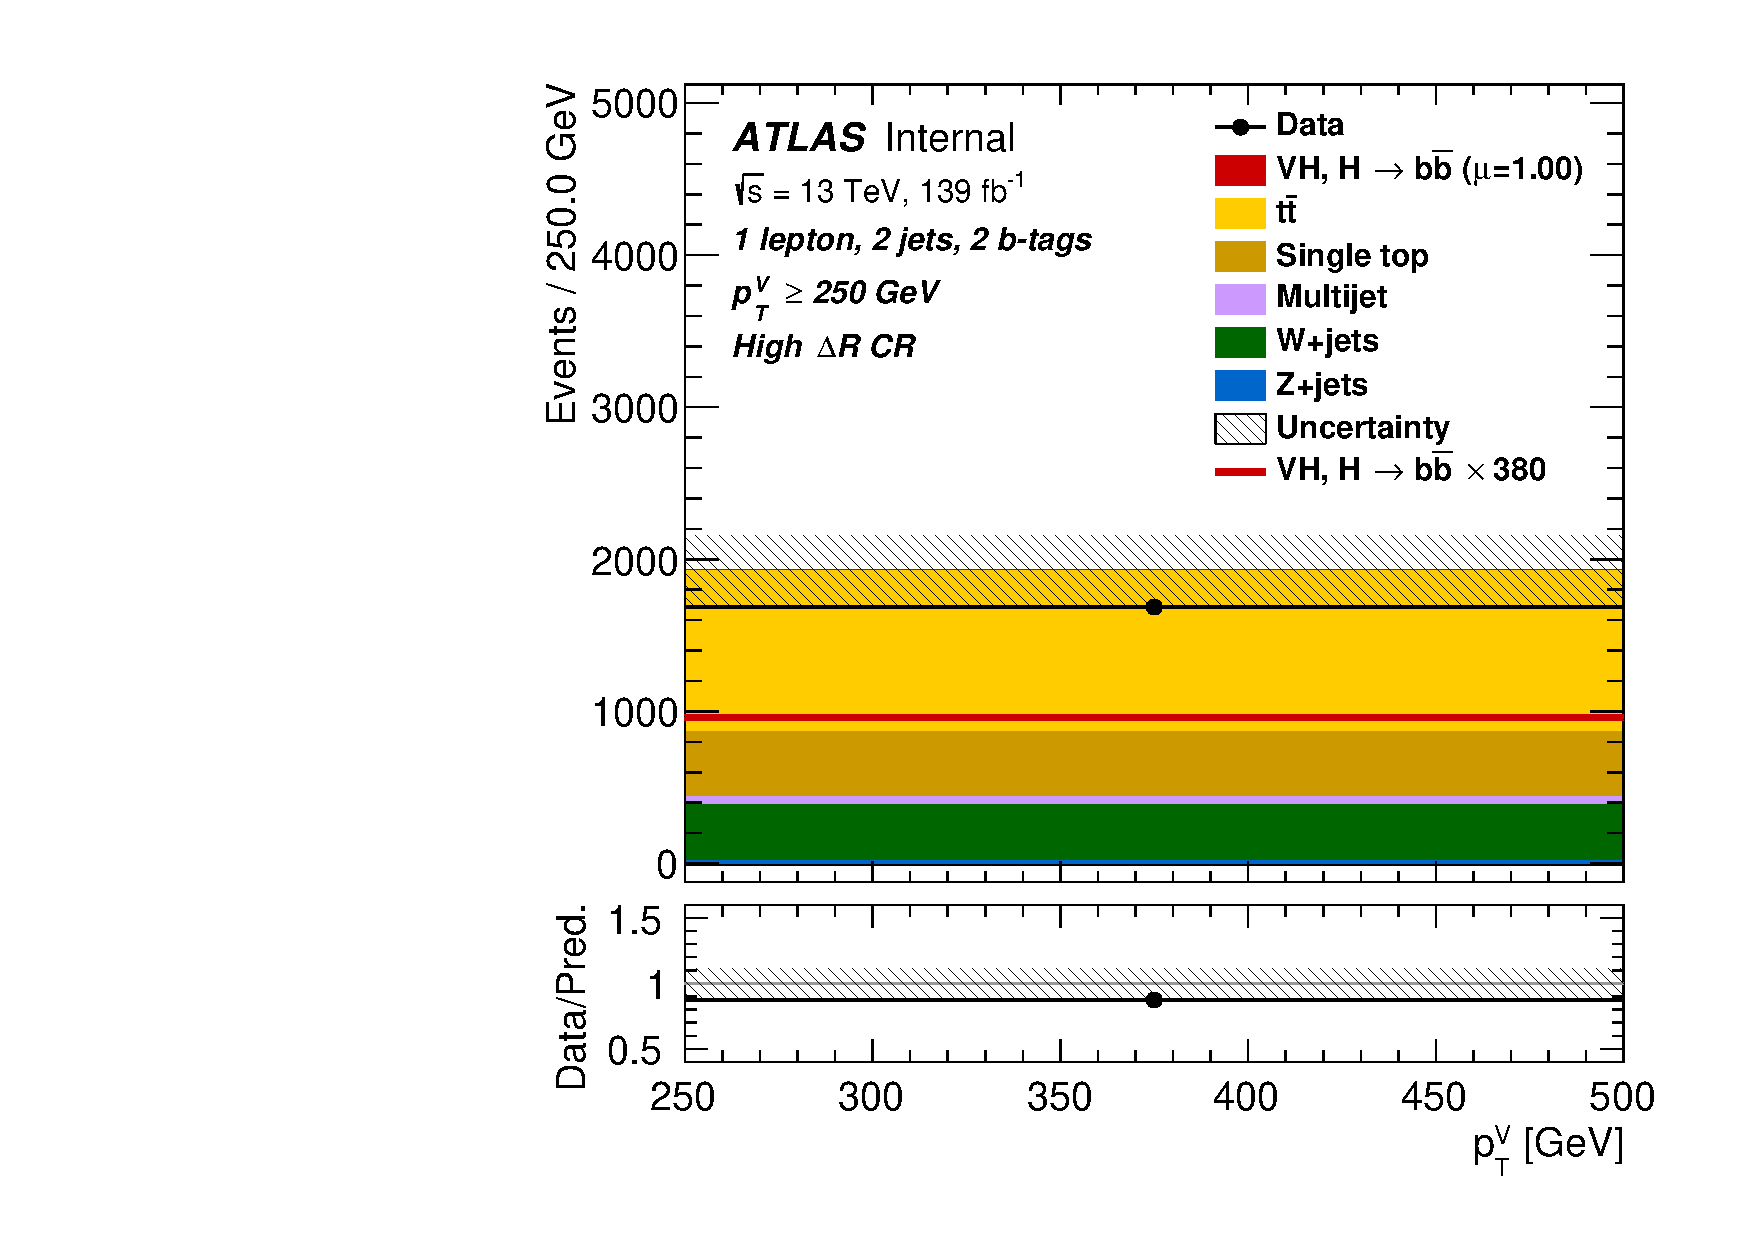
\includegraphics[width=.3\textwidth]{final_fit_mva/prefit/Region_BMin250_Y6051_DCRHigh_T2_L1_distpTV_J2_Prefit} \\

    % middle row
    \includegraphics[width=.3\textwidth]{final_fit_mva/prefit/Region_BMax250_BMin150_Y6051_DSR_T2_L1_distmva_J2_Prefit}%
    & \includegraphics[width=.3\textwidth]{final_fit_mva/prefit/Region_BMin250_Y6051_DSR_T2_L1_distmva_J2_Prefit} \\

    % bottom row
    \includegraphics[width=.3\textwidth]{final_fit_mva/prefit/Region_BMax250_BMin150_Y6051_DCRLow_T2_L1_distpTV_J2_Prefit}%
    & \includegraphics[width=.3\textwidth]{final_fit_mva/prefit/Region_BMin250_Y6051_DCRLow_T2_L1_distpTV_J2_Prefit} \\
  \end{tabular}
  \caption{Pre-fit distributions in the 1 lepton 2 jet channel.}
\end{figure}
\begin{figure}
  \centering
  \begin{tabular}{cc}
    % top row
    \includegraphics[width=.3\textwidth]{final_fit_mva/prefit/Region_BMax250_BMin150_Y6051_DCRHigh_T2_L1_distpTV_J3_Prefit}%
    & \includegraphics[width=.3\textwidth]{final_fit_mva/prefit/Region_BMin250_Y6051_DCRHigh_T2_L1_distpTV_J3_Prefit} \\

    % middle row
    \includegraphics[width=.3\textwidth]{final_fit_mva/prefit/Region_BMax250_BMin150_Y6051_DSR_T2_L1_distmva_J3_Prefit}%
    & \includegraphics[width=.3\textwidth]{final_fit_mva/prefit/Region_BMin250_Y6051_DSR_T2_L1_distmva_J3_Prefit} \\

    % bottom row
    \includegraphics[width=.3\textwidth]{final_fit_mva/prefit/Region_BMax250_BMin150_Y6051_DCRLow_T2_L1_distpTV_J3_Prefit}%
    & \includegraphics[width=.3\textwidth]{final_fit_mva/prefit/Region_BMin250_Y6051_DCRLow_T2_L1_distpTV_J3_Prefit} \\
  \end{tabular}
  \caption{Pre-fit distributions in the 1 lepton 3 jet channel.}
\end{figure}
\begin{figure}
  \centering
  \begin{tabular}{cc}
    % top row
    \includegraphics[width=.33\textwidth]{final_fit_mva/prefit/Region_BMax150_BMin75_Y6051_DCRHigh_T2_L2_distpTV_J2_Prefit}%
    \includegraphics[width=.33\textwidth]{final_fit_mva/prefit/Region_BMax250_BMin150_Y6051_DCRHigh_T2_L2_distpTV_J2_Prefit}%
    & \includegraphics[width=.33\textwidth]{final_fit_mva/prefit/Region_BMin250_Y6051_DCRHigh_T2_L2_distpTV_J2_Prefit} \\

    % middle row
    \includegraphics[width=.33\textwidth]{final_fit_mva/prefit/Region_BMax150_BMin75_Y6051_DSR_T2_L2_distmva_J2_Prefit}%
    \includegraphics[width=.33\textwidth]{final_fit_mva/prefit/Region_BMax250_BMin150_Y6051_DSR_T2_L2_distmva_J2_Prefit}%
    & \includegraphics[width=.33\textwidth]{final_fit_mva/prefit/Region_BMin250_Y6051_DSR_T2_L2_distmva_J2_Prefit} \\

    % bottom row
    \includegraphics[width=.33\textwidth]{final_fit_mva/prefit/Region_BMax150_BMin75_Y6051_DCRLow_T2_L2_distpTV_J2_Prefit}%
    \includegraphics[width=.33\textwidth]{final_fit_mva/prefit/Region_BMax250_BMin150_Y6051_DCRLow_T2_L2_distpTV_J2_Prefit}%
    & \includegraphics[width=.33\textwidth]{final_fit_mva/prefit/Region_BMin250_Y6051_DCRLow_T2_L2_distpTV_J2_Prefit} \\
  \end{tabular}
  \caption{Pre-fit distributions in the 2--lepton channel in the  2--jet
    region.}
  \label{fig:2lep-2jet-prefit}
\end{figure}
\begin{figure}
  \centering
  \begin{tabular}{cc}
    % top row
    \includegraphics[width=.3\textwidth]{final_fit_mva/prefit/Region_BMax150_BMin75_incJet1_Y6051_DCRHigh_T2_L2_distpTV_J3_Prefit}%
    \includegraphics[width=.3\textwidth]{final_fit_mva/prefit/Region_BMax250_BMin150_incJet1_Y6051_DCRHigh_T2_L2_distpTV_J3_Prefit}%
    & \includegraphics[width=.3\textwidth]{final_fit_mva/prefit/Region_BMin250_incJet1_Y6051_DCRHigh_T2_L2_distpTV_J3_Prefit} \\

    % middle row
    \includegraphics[width=.3\textwidth]{final_fit_mva/prefit/Region_BMax150_BMin75_incJet1_Y6051_DSR_T2_L2_distmva_J3_Prefit}%
    \includegraphics[width=.3\textwidth]{final_fit_mva/prefit/Region_BMax250_BMin150_incJet1_Y6051_DSR_T2_L2_distmva_J3_Prefit}%
    & \includegraphics[width=.3\textwidth]{final_fit_mva/prefit/Region_BMin250_incJet1_Y6051_DSR_T2_L2_distmva_J3_Prefit} \\

    % bottom row
    \includegraphics[width=.3\textwidth]{final_fit_mva/prefit/Region_BMax150_BMin75_incJet1_Y6051_DCRLow_T2_L2_distpTV_J3_Prefit}%
    \includegraphics[width=.3\textwidth]{final_fit_mva/prefit/Region_BMax250_BMin150_incJet1_Y6051_DCRLow_T2_L2_distpTV_J3_Prefit}%
    & \includegraphics[width=.3\textwidth]{final_fit_mva/prefit/Region_BMin250_incJet1_Y6051_DCRLow_T2_L2_distpTV_J3_Prefit} \\
  \end{tabular}
  \caption{Pre-fit distributions in the 2--lepton channel in the  3+--jet
    region.}
  \label{fig:2lep-3pjet-prefit}
\end{figure}





